% !TeX program = xelatex
%DIF LATEXDIFF DIFFERENCE FILE
%DIF DEL old/main.tex   Wed Oct 14 20:06:59 2026
%DIF ADD main.tex       Wed Oct 14 18:45:56 2026
\documentclass[a4paper,11pt]{article}

\usepackage[a4paper,left=12mm,textwidth=156mm,marginparsep=2.5mm,marginparwidth=36mm,top=14mm,bottom=14mm]{geometry}
\usepackage{newtxtext,newtxmath}
\usepackage{xeCJK}
\setCJKmainfont{Noto Sans CJK SC}[Script=CJK,Path=/usr/share/fonts/opentype/noto/,Extension=.ttc,UprightFont=NotoSansCJK-Regular,BoldFont=NotoSansCJK-Bold,FontIndex=2,BoldFeatures={FontIndex=2}]
\setCJKsansfont{Noto Sans CJK SC}[Script=CJK,Path=/usr/share/fonts/opentype/noto/,Extension=.ttc,UprightFont=NotoSansCJK-Regular,BoldFont=NotoSansCJK-Bold,FontIndex=2,BoldFeatures={FontIndex=2}]
\setCJKmonofont{Noto Sans CJK SC}[Script=CJK,Path=/usr/share/fonts/opentype/noto/,Extension=.ttc,UprightFont=NotoSansCJK-Regular,BoldFont=NotoSansCJK-Bold,FontIndex=2,BoldFeatures={FontIndex=2}]

\usepackage{amsmath}
\usepackage{booktabs,longtable,tabularx,array,multirow}
\usepackage{graphicx,float}
\usepackage{algorithm}
\usepackage{algpseudocode}
\usepackage{xcolor}
\usepackage{microtype}
\usepackage{enumitem}
\usepackage{caption}
\usepackage{url}
\usepackage{hyperref}
\usepackage{marginfix}
\let\DIForigmarginpar\marginpar
\renewcommand{\marginpar}[1]{\DIForigmarginpar{\color{black}#1}}

\graphicspath{{figures/}{./}}
\hypersetup{
  colorlinks=true,
  linkcolor=black,
  citecolor=blue!60!black,
  urlcolor=blue!60!black,
%DIF 26c26
%DIF <   pdftitle={Coverage Path Planning for a Swing-Arm Concrete Troweling Robot in Complex Environments},
%DIF -------
  pdftitle={BiRect: Bidirectional Rectangular Coverage Path Planning for a Swing-Arm Concrete Troweling Robot}, %DIF > 
%DIF -------
  pdfauthor={Yuzhi Pan}
}
\captionsetup{font=small,labelfont=bf}
\setlength{\parindent}{1.5em}
\setlength{\parskip}{0.2em}
\setcounter{secnumdepth}{3}
\setcounter{tocdepth}{2}

\title{\DIFaddbegin \DIFadd{BiRect: Bidirectional Rectangular }\DIFaddend Coverage Path Planning for a Swing-Arm Concrete Troweling Robot\DIFdelbegin \DIFdel{in Complex Environments}\DIFdelend }
\author{Yuzhi Pan}
\date{}
%DIF PREAMBLE EXTENSION ADDED BY LATEXDIFF
%DIF UNDERLINE PREAMBLE %DIF PREAMBLE
\RequirePackage[normalem]{ulem} %DIF PREAMBLE
\RequirePackage{color}\definecolor{RED}{rgb}{1,0,0}\definecolor{BLUE}{rgb}{0,0,1} %DIF PREAMBLE
\providecommand{\DIFaddtex}[1]{{\protect\color{blue}#1}} %DIF PREAMBLE
\providecommand{\DIFdeltex}[1]{{\protect\color{red}\sout{#1}}} %DIF PREAMBLE
%DIF SAFE PREAMBLE %DIF PREAMBLE
\providecommand{\DIFaddbegin}{} %DIF PREAMBLE
\providecommand{\DIFaddend}{} %DIF PREAMBLE
\providecommand{\DIFdelbegin}{} %DIF PREAMBLE
\providecommand{\DIFdelend}{} %DIF PREAMBLE
\providecommand{\DIFmodbegin}{} %DIF PREAMBLE
\providecommand{\DIFmodend}{} %DIF PREAMBLE
%DIF FLOATSAFE PREAMBLE %DIF PREAMBLE
\providecommand{\DIFaddFL}[1]{\DIFadd{#1}} %DIF PREAMBLE
\providecommand{\DIFdelFL}[1]{\DIFdel{#1}} %DIF PREAMBLE
\providecommand{\DIFaddbeginFL}{} %DIF PREAMBLE
\providecommand{\DIFaddendFL}{} %DIF PREAMBLE
\providecommand{\DIFdelbeginFL}{} %DIF PREAMBLE
\providecommand{\DIFdelendFL}{} %DIF PREAMBLE
%DIF HYPERREF PREAMBLE %DIF PREAMBLE
\providecommand{\DIFadd}[1]{\texorpdfstring{\DIFaddtex{#1}}{#1}} %DIF PREAMBLE
\providecommand{\DIFdel}[1]{\texorpdfstring{\DIFdeltex{#1}}{}} %DIF PREAMBLE
%DIF AMSMATHULEM PREAMBLE %DIF PREAMBLE
\makeatletter %DIF PREAMBLE
\let\sout@orig\sout %DIF PREAMBLE
\renewcommand{\sout}[1]{\ifmmode\text{\sout@orig{\ensuremath{#1}}}\else\sout@orig{#1}\fi} %DIF PREAMBLE
\makeatother %DIF PREAMBLE
%DIF COLORLISTINGS PREAMBLE %DIF PREAMBLE
\RequirePackage{listings} %DIF PREAMBLE
\RequirePackage{color} %DIF PREAMBLE
\lstdefinelanguage{DIFcode}{ %DIF PREAMBLE
%DIF DIFCODE_UNDERLINE %DIF PREAMBLE
  moredelim=[il][\color{red}\sout]{\%DIF\ <\ }, %DIF PREAMBLE
  moredelim=[il][\color{blue}\uwave]{\%DIF\ >\ } %DIF PREAMBLE
} %DIF PREAMBLE
\lstdefinestyle{DIFverbatimstyle}{ %DIF PREAMBLE
	language=DIFcode, %DIF PREAMBLE
	basicstyle=\ttfamily, %DIF PREAMBLE
	columns=fullflexible, %DIF PREAMBLE
	keepspaces=true %DIF PREAMBLE
} %DIF PREAMBLE
\lstnewenvironment{DIFverbatim}[1][]{\lstset{style=DIFverbatimstyle}}{} %DIF PREAMBLE
\lstnewenvironment{DIFverbatim*}[1][]{\lstset{style=DIFverbatimstyle,showspaces=true}}{} %DIF PREAMBLE
\lstset{extendedchars=\true}

%DIF END PREAMBLE EXTENSION ADDED BY LATEXDIFF

\begin{document}

\thispagestyle{empty}
\begin{center}
{\Large\bfseries 修订对照说明}
\end{center}
\vspace{1.2em}
\noindent 图例：红色删除线表示被删除的原文；蓝色文字表示新增内容；边注用中文说明修改理由，对应导师意见中的一条以及具体改法。
\vspace{0.8em}
\noindent 本次修订共 81 处，其中 A 类 73 处，B 类 8 处。B 类编号为 25、38、48、49、63、67、70、81，其余编号为 A 类。
\vspace{0.8em}
\noindent A 类是措辞、引用、公式文字、图注和表格排版。B 类只重画或新增基于已有几何或数据的图，不改变实验数字。
\clearpage
\maketitle

\marginpar{\scriptsize [1] 将标题改为 BiRect，并锁定 base、disc、swing arm、route、trajectory 的用词。}\begin{abstract}
\DIFdelbegin \DIFdel{Concrete floor troweling must cover large areas within a limited construction window. In workspaces partitioned by }\DIFdelend \DIFaddbegin \DIFadd{Compared with center-mounted and front-mounted configurations, a swing-arm robot can keep the base clear of }\marginpar{\scriptsize [2] 把摘要开头改成摆臂优势、固定足迹缺口、因此提出 BiRect。}\DIFaddend walls, columns, and openings \DIFdelbegin \DIFdel{, a swing-arm robot must plan both base traversal and end-disc coverage. Most existing }\DIFdelend \DIFaddbegin \DIFadd{while the disc covers lateral regions and narrow passages during large-area, repetitive troweling. Existing }\DIFaddend coverage path planning methods \DIFdelbegin \DIFdel{assume }\DIFdelend \DIFaddbegin \DIFadd{still focus on regular sites or agricultural fields with }\DIFaddend a fixed tool footprint\DIFdelbegin \DIFdel{and therefore cannot represent the }\DIFdelend \DIFaddbegin \DIFadd{; they do not account for an active swing arm or for the }\DIFaddend time-varying \DIFdelbegin \DIFdel{sweep produced by an actuated arm or generate a continuous, executable route in a }\DIFdelend \DIFaddbegin \DIFadd{disc sweep on a }\DIFaddend complex map. This paper \DIFdelbegin \DIFdel{presents a hierarchical coverage path planning method for }\DIFdelend \DIFaddbegin \DIFadd{therefore presents BiRect. It proposes, for a }\marginpar{\scriptsize [3] 将贡献改为提出、引入、开发三句，实验数字未改。}\DIFaddend known two-dimensional \DIFdelbegin \DIFdel{environments with obstacles. The method first organizes the workspace using axis-aligned rectangular candidates generated in two scan directions, followed by }\DIFdelend \DIFaddbegin \DIFadd{obstacle map, joining the visitation order over a complex free space and coordinated base and swing-arm motion into one executable route. It introduces bidirectional rectangular candidates, together with }\DIFaddend hole filling and connectivity completion\DIFdelbegin \DIFdel{. It then determines a global visitation order and synthesizes coordinated base--arm motions. Coverage is evaluated }\DIFdelend \DIFaddbegin \DIFadd{, so that an irregular free space becomes rectangles that a swing arm can visit continuously. It develops local sweeping that varies with arm angle; the coverage ratio and execution time are computed }\DIFaddend from the actual \DIFdelbegin \DIFdel{area swept by the circular troweling }\DIFdelend \DIFaddbegin \DIFadd{sweep of the circular }\DIFaddend disc along the complete trajectory, while the \DIFaddbegin \DIFadd{coupled }\marginpar{\scriptsize [5] 在 effects 前插入 coupled。}\DIFaddend effects of base speed and arm angular velocity on sweep continuity and execution time are \DIFdelbegin \DIFdel{explicitly included. On two test maps, }\DIFdelend \DIFaddbegin \DIFadd{further revealed. Experiments showed that }\marginpar{\scriptsize [4] 将摘要中两幅测试图的起句改为实验结果表明。}\marginpar{\scriptsize [6] 将 explicitly included 改为 further revealed。}\DIFaddend the proposed method achieves full-trajectory coverage ratios of 94.11\% and 95.73\%, respectively, and both generated routes pass the motion-feasibility checks. By contrast, the connecting segments produced by a fixed-width baseline leave the valid workspace by 4.51~m$^2$ and 20.00~m$^2$, making those routes non-executable. Experiments \DIFdelbegin \DIFdel{on five maps }\marginpar{\scriptsize [7] 删去 on five maps。}\DIFdelend further show that the bidirectional candidate strategy attains the highest mean full-trajectory coverage ratio (94.32\%) and the lowest mean total execution time (2316.60~s). These results support integrating complex-map decomposition, active arm motion, and continuous swept-area evaluation within a single planning pipeline. Validation in dynamic construction environments and on a physical robot remains future work.
\end{abstract}

\noindent\textbf{Keywords:} coverage path planning; construction robotics; concrete troweling; swing-arm robot; area decomposition

\section{Introduction}

Construction work entails substantial safety and health risks. The U.S. Bureau of Labor Statistics reported 1,032 fatal occupational injuries in construction and extraction occupations in 2024; common events included falls, slips, trips, and transportation incidents involving construction vehicles or machinery \cite{bls2024}. Beyond traumatic injuries, work with silica-containing materials such as concrete and mortar can expose workers to high concentrations of respirable crystalline silica over long periods, increasing the risks of silicosis, lung cancer, and chronic obstructive pulmonary disease \cite{niosh2024}. Concrete floor leveling and troweling further combine a large work area, repeated passes, and a narrow time window governed by concrete setting. Manual work therefore requires sustained physical exertion and repetitive motion. Field physiological measurements of concrete slab placing and finishing crews showed that most manual workers experienced high energy expenditure and cardiopulmonary demand, with a greater risk of physical fatigue than equipment operators \cite{abdelhamid1999}. \DIFdelbegin \DIFdel{Work quality }\DIFdelend \DIFaddbegin \DIFadd{Surface finish }\DIFaddend also depends on operator experience, proficiency, and moment-to-moment condition \cite{albers2004,kobayashi1996}. Releasing workers from hazardous, repetitive, and physically demanding floor operations while improving the consistency of the finished surface is therefore a problem of direct engineering and social value for construction robotics.

Floor-troweling robots provide a practical route toward mechanization. Early field trials showed that a remotely operated troweling robot could perform multiple operations from wood floating to steel troweling. It treated approximately 1,000~m$^2$ across five sites and achieved an average productivity of about 317~m$^2$/h under the reported test conditions \cite{kobayashi1996}. For an order-of-magnitude comparison, the average production rate of manual steel troweling is approximately 13.9~m$^2$/h \cite{methvin2026}; the reported robotic rate is therefore about 22.8 times the rate of one manual worker. Subsequent work introduced electric actuation, laser localization, task planning, and remote monitoring to ride-on power trowels, allowing them to follow specified paths within a predefined floor area \cite{hwangbo1999}.

Most existing troweling robots use a \DIFdelbegin \DIFdel{disc mounted beneath or in front of the base}\DIFdelend \DIFaddbegin \DIFadd{center-mounted or front-mounted disc}\marginpar{\scriptsize [11] 把三类命名为 center-mounted、front-mounted、swing-arm，并改了图注用词。}\DIFaddend . Because the tool remains fixed relative to the base, the base path largely determines the tool path, and back-and-forth routes can be planned with a fixed working width \cite{kobayashi1996,hwangbo1999}. Swing-arm configurations have recently attracted attention because they enlarge the end-disc workspace without requiring a large base. Such a robot can place its circular disc beside the base or into locally constrained regions while the base remains clear of walls, columns, and openings, thereby partially decoupling the traversable base path from the tool trajectory. The arm can also increase the effective coverage width. For a fixed-disc platform, the nominal width of a straight pass is mainly limited by the disc diameter. A swing-arm platform can instead move the disc laterally while the base advances, so that the effective width depends on the arm length, angular range, and disc diameter and can exceed the disc diameter \cite{lin2025}. At the same base speed, provided that the swing frequency keeps consecutive sweeps contiguous without introducing gaps, the theoretical covered area per unit time can increase from approximately $v(2R)$ for a fixed disc to $v w_{\mathrm{eff}}$ for a swing arm, where $w_{\mathrm{eff}}>2R$. Previous coverage-planning research likewise shows that repeated coverage, average velocity, and the smoothness of turns jointly affect task time and energy consumption \cite{galceran2013,lee2011}. The swing-arm configuration may also reduce unnecessary driving and sharp turns on wet concrete and provide more admissible poses near corners, narrow-passage entrances, and obstacles \cite{lin2025}.

\begin{figure}[htbp]
  \centering
  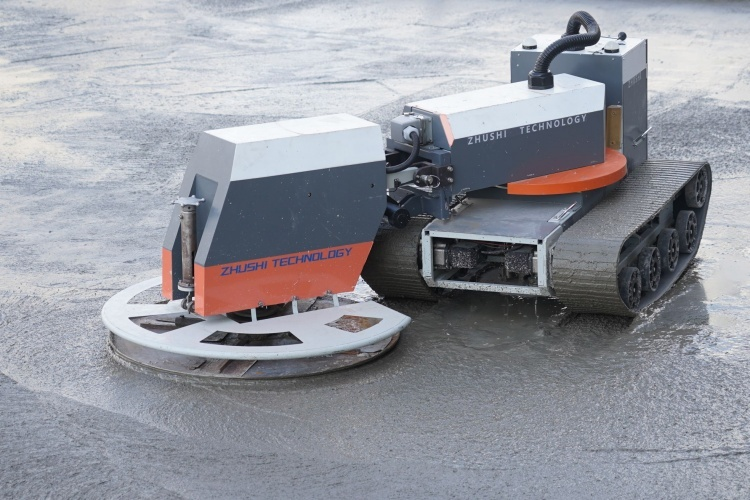
\includegraphics[width=0.82\linewidth]{figure_1_swing_arm_troweling_robot_photo.jpg}
  \caption{A swing-arm troweling robot operating on site. The tracked base, swing arm and actuator, and circular end disc are visible. Image source: Shangguan News; photograph provided by China Construction Eighth Engineering Division.}
  \label{fig:robot-photo}
\end{figure}

Mechanization and teleoperation, however, do not by themselves provide autonomy. A human teleoperator must continuously observe the floor and machine state while coordinating translation, steering, and troweling. In spaces divided by walls, columns, embedded components, and openings, occluded views and fragmented passages increase the burden of global route selection and can cause backtracking, detours, missed regions, and repeated work. Experiments with teleoperated mobile robots also show that manual driving time increases with environmental difficulty and depends on operator skill and the level of obstacle-avoidance assistance \cite{storms2016}. Existing swing-arm systems commonly rely on human--robot cooperation or predefined trajectories and do not yet generate complete coverage routes automatically for complex construction maps \cite{lin2025}. Continuous teleoperation also requires a skilled operator to remain on duty, adding training and on-site supervision costs. Empirical studies of construction-robot adoption further identify economic factors, work culture, and uncertain business returns as barriers to deployment \cite{ocs2024,delgado2019}. Without autonomous coverage planning, these operational burdens remain even after the troweling process is mechanized.

This task is an instance of coverage path planning (CPP): the tool must sweep the target area while avoiding obstacles and controlling missed coverage, repeated coverage, transfer distance, and execution time \cite{galceran2013}. Existing approaches include back-and-forth sweeps after cellular decomposition\marginpar{\scriptsize [8] 把引言引用拆到细胞分解、多边形、栅格和农业条带各半句，没有增加文献。} \DIFdelbegin \DIFdel{, }\DIFdelend \DIFaddbegin \DIFadd{\mbox{%DIFAUXCMD
\cite{choset1998,bahnemann2021}}\hskip0pt%DIFAUXCMD
, decomposition and transfers on polygons with holes \mbox{%DIFAUXCMD
\cite{polygoncoverage}}\hskip0pt%DIFAUXCMD
, }\DIFaddend grid or spanning-tree traversal \DIFaddbegin \DIFadd{\mbox{%DIFAUXCMD
\cite{gabriely2001,nobleo}}\hskip0pt%DIFAUXCMD
}\DIFaddend , and strip generation with curvature-constrained connections for fixed-width implements \DIFdelbegin \DIFdel{. These approaches respectively address polygonal or occupancy-grid maps, regular regions, and }\DIFdelend \DIFaddbegin \DIFadd{in }\DIFaddend applications such as agriculture \DIFdelbegin \DIFdel{in which the tool footprint is fixed \mbox{%DIFAUXCMD
\cite{choset1998,gabriely2001,bahnemann2021,polygoncoverage,mier2023,fields2cover,nobleo}}\hskip0pt%DIFAUXCMD
}\DIFdelend \DIFaddbegin \DIFadd{\mbox{%DIFAUXCMD
\cite{mier2023,fields2cover}}\hskip0pt%DIFAUXCMD
}\DIFaddend . Mobile-manipulator methods can plan local motions for a base and an end tool \DIFaddbegin \DIFadd{\mbox{%DIFAUXCMD
\cite{thakar2022}}\hskip0pt%DIFAUXCMD
}\DIFaddend , while SatAOI can identify the workable area of a swing-arm troweling robot in an obstacle map \DIFaddbegin \DIFadd{\mbox{%DIFAUXCMD
\cite{lin2025}}\hskip0pt%DIFAUXCMD
}\DIFaddend ; neither, however, provides a complete continuous coverage route for a complex two-dimensional floor\DIFdelbegin \DIFdel{\mbox{%DIFAUXCMD
\cite{lin2025,thakar2022}}\hskip0pt%DIFAUXCMD
}\DIFdelend . Section~\ref{sec:related-work} gives a detailed classification and discusses these boundaries.

CPP for a swing-arm troweling robot introduces three interdependent requirements. First, the planner must represent a complex free space containing openings, dense obstacles, and narrow connections. Second, at a fixed base pose, it must distinguish the disc positions and whole-robot collision states associated with different arm angles. Third, while the base moves continuously, actual coverage must be determined from arm angular velocity and the continuous disc sweep rather than from a static reachability envelope. \DIFaddbegin \DIFadd{A static reachability envelope is the region the arm can touch in some poses and does not include the time course of base travel and swing-arm motion. }\marginpar{\scriptsize [34] 在引言定义 static reachability envelope，后文再指回该定义。}\DIFaddend Simply dilating the base path into a constant-width strip cannot satisfy all three requirements. Consequently, prior work lacks a complete planning chain from a construction map through decomposition and visitation order to coordinated base--arm motion and end-tool coverage evaluation.

\DIFdelbegin \DIFdel{To close this gap, this paper presents a hierarchical CPP method for known two-dimensional environments with obstacles. Bidirectional rectangular candidates and connectivity completion represent the complex free space. A }\DIFdelend \DIFaddbegin \DIFadd{This paper proposes BiRect, a hierarchical coverage path planning method that places bidirectional rectangular decomposition, the visitation order on a }\marginpar{\scriptsize [9] 将引言贡献收成一句，并与论文结构段合并。}\DIFaddend feasible transition graph\DIFdelbegin \DIFdel{then organizes global visitation, and first visits and repeated transit visits are instantiated as local swing-assisted coverage motions and transfer motions, respectively. Finally, }\DIFdelend \DIFaddbegin \DIFadd{, and }\DIFaddend the coverage ratio and execution time \DIFdelbegin \DIFdel{are }\DIFdelend computed from the \DIFdelbegin \DIFdel{region }\DIFdelend \DIFaddbegin \DIFadd{area }\DIFaddend actually swept by the circular disc \DIFdelbegin \DIFdel{along the continuous trajectory. The same robot model is thus used for map representation, arm behavior}\DIFdelend \DIFaddbegin \DIFadd{in one chain, using the same base--swing-arm--disc model for the map}\DIFaddend , \DIFaddbegin \DIFadd{local motion, }\DIFaddend and trajectory evaluation.

The remainder of the paper is organized as follows. Section~\ref{sec:related-work} reviews the development of concrete-troweling robots and the challenges posed by obstacle-rich construction environments, compares representative CPP methods, and summarizes the unresolved research gap. Section~\ref{sec:methodology} presents the robot and environment models, rectangular-candidate decomposition, connectivity completion, global visitation, and swing-assisted coverage within each rectangle. Section~\ref{sec:experiments} evaluates the method through a baseline comparison, candidate-scan strategy experiments, and a speed-sensitivity study. Section~\ref{sec:conclusion} summarizes the experimentally supported contributions, limitations, and future work.

\section{Related Work}
\label{sec:related-work}

\subsection{Concrete Troweling Robots and Application Challenges}

After concrete has been placed and initially leveled, it must be troweled repeatedly before setting and hardening. Troweling removes local height variations and rough texture, redistributes the surface paste, and produces a flat, dense finish through compaction and polishing. The operation covers a large area and is highly repetitive, while its start time, speed, and number of passes are constrained by the state of concrete setting. Starting too early can disturb an unstable surface; starting too late can prevent the desired flatness and finish. Site practice has therefore long depended on the experience and continuous involvement of skilled workers \cite{albers2004,kobayashi1996}. A troweling robot moves the disc and treats the surface at a relatively stable speed and cadence, reducing physical workload and the effect of worker-state variability on quality consistency \cite{kobayashi1996,shin2003}. Its role is thus not merely to replace a hand tool, but to convert a process that requires continuous manual operation into one that a mechanical system can execute consistently.

\DIFdelbegin \DIFdel{Existing troweling robots can be grouped into three broad configurations according to the position of the disc relative to the base.
In the first, the circular disc is mounted }\DIFdelend \DIFaddbegin \DIFadd{The evolution of concrete-troweling equipment can be understood along two axes: the disc--base relationship and the mode of control.
}

\DIFadd{Along the disc--base relationship, existing troweling robots fall into three configurations. A center-mounted disc lies }\marginpar{\scriptsize [10] 将两轴句前移，再按盘与基座的关系和控制方式分段。}\DIFaddend under or near the center of the base\DIFdelbegin \DIFdel{. This compact and mechanically stable arrangement is suitable for fixed-width operation on open floors, but the tool footprint essentially translates with the base path. In the second, the disc is mounted in front of }\DIFdelend \DIFaddbegin \DIFadd{, as on the ride-on twin-rotor machine \mbox{%DIFAUXCMD
\cite{hwangbo1999} }\hskip0pt%DIFAUXCMD
and on }\DIFaddend the \DIFdelbegin \DIFdel{base, making the forward work area easy for an operator or sensor to observe, but requiring the base to approach the treatment boundary and offering limited lateral reach. In the third, the disc is mounted }\DIFdelend \DIFaddbegin \DIFadd{twin-disc machine whose discs sit under the body and whose travel follows disc attitude \mbox{%DIFAUXCMD
\cite{shin2003}}\hskip0pt%DIFAUXCMD
. A front-mounted arrangement places troweling discs at both the front and the rear of the travel mechanism; the discs stay fixed relative to the base and have no active lateral motion \mbox{%DIFAUXCMD
\cite{kobayashi1996}}\hskip0pt%DIFAUXCMD
. A swing-arm configuration places the disc }\DIFaddend at the end of \DIFdelbegin \DIFdel{a swing arm . Controlled relative motion between the base and disc then allows the robot to cover lateral regions, areas near obstacles, and narrow-passage entrances while the base remains at a safe distance. This paper focuses on the third configuration for two reasons. The arm can actively reposition the disc relative to the base, making coverage near }\DIFdelend \DIFaddbegin \DIFadd{an actively rotating arm \mbox{%DIFAUXCMD
\cite{lin2025}}\hskip0pt%DIFAUXCMD
. The swing arm can send the disc into regions beside }\DIFaddend walls, columns, openings, and narrow passages \DIFdelbegin \DIFdel{more flexible. In addition, at }\DIFdelend \DIFaddbegin \DIFadd{while the base stays clear of them. When consecutive sweeps remain contiguous, }\DIFaddend the same base speed \DIFdelbegin \DIFdel{and with a contiguous sweep, the }\DIFdelend \DIFaddbegin \DIFadd{can give an }\DIFaddend effective coverage width \DIFdelbegin \DIFdel{can exceed }\DIFdelend \DIFaddbegin \DIFadd{larger than }\DIFaddend the disc diameter\DIFdelbegin \DIFdel{, increasing the area treated per unit time \mbox{%DIFAUXCMD
\cite{lin2025,galceran2013,lee2011}}\hskip0pt%DIFAUXCMD
. Both advantages arise }\DIFdelend \DIFaddbegin \DIFadd{. This configuration has received increasing attention in recent construction-robot research \mbox{%DIFAUXCMD
\cite{lin2025}}\hskip0pt%DIFAUXCMD
. These advantages come }\marginpar{\scriptsize [12] 改为陈述摆臂已有的两条优势，不再写聚焦第三类。}\DIFaddend from coordinating base translation with \DIFdelbegin \DIFdel{arm swinging }\DIFdelend \DIFaddbegin \DIFadd{swing-arm motion }\DIFaddend and cannot be \DIFdelbegin \DIFdel{captured by a conventional }\DIFdelend \DIFaddbegin \DIFadd{represented by a }\DIFaddend fixed-width strip model.

\begin{figure}[htbp]
  \centering
  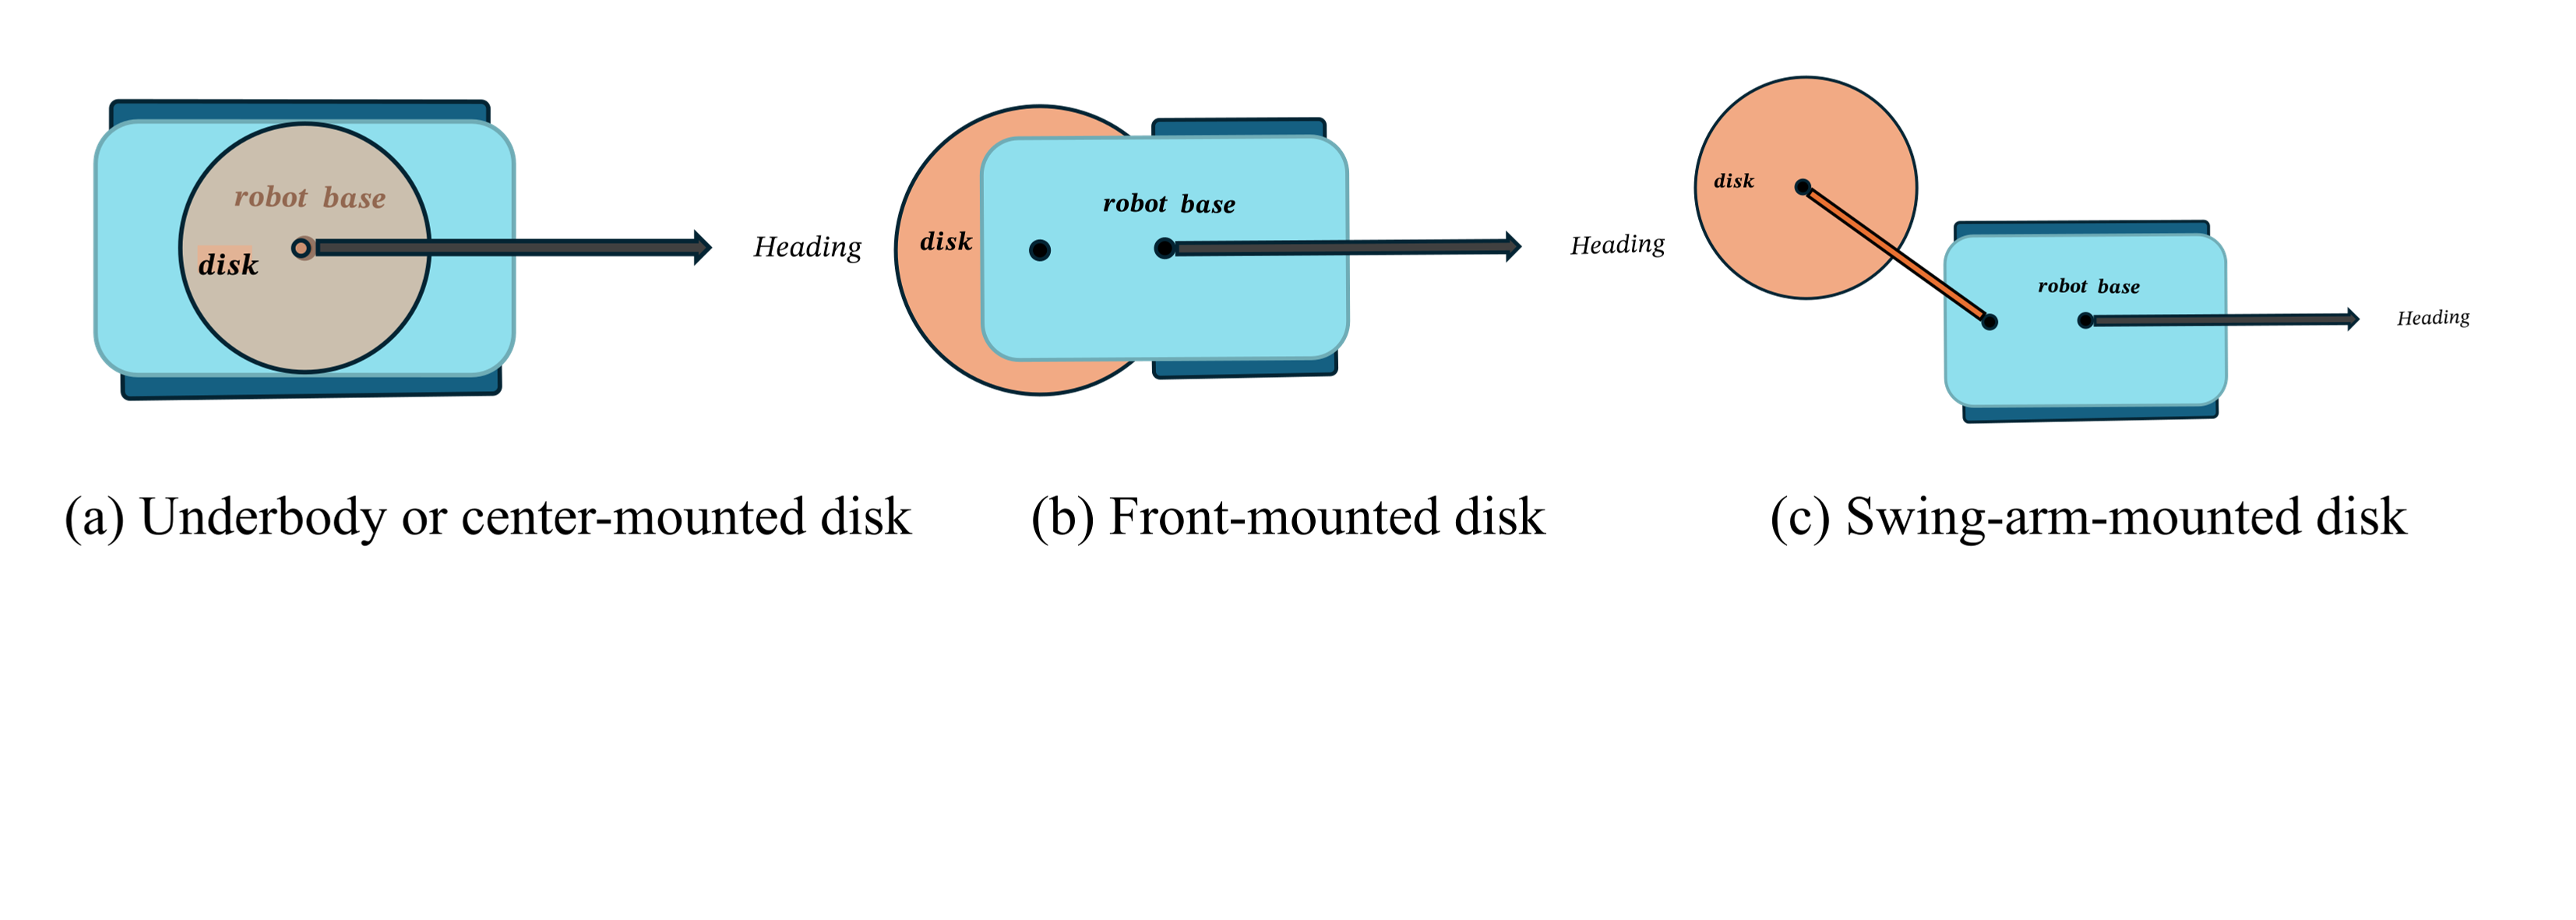
\includegraphics[width=0.92\linewidth]{figure_2_disc_vehicle_relationships.png}
  \caption{Three arrangements of the troweling disc relative to the base: (a) \DIFdelbeginFL \DIFdelFL{disc beneath or near the center of the base}\DIFdelendFL \DIFaddbeginFL \DIFaddFL{center-mounted}\DIFaddendFL ; (b) front-mounted\DIFdelbeginFL \DIFdelFL{disc}\DIFdelendFL ; and (c) \DIFdelbeginFL \DIFdelFL{disc at the end of a swing arm}\DIFdelendFL \DIFaddbeginFL \DIFaddFL{swing-arm}\DIFaddendFL . Arrows indicate the direction of base travel.}
  \label{fig:disc-configurations}
\end{figure}

The \DIFdelbegin \DIFdel{swing-arm arrangement enlarges the platform workspace by mounting the disc at the end of a rotating long arm. Unlike a disc fixed beneath or in front of the base, the arm can treat lateral regions while the base maintains clearance and can create multiple base--tool configurations by changing its angle. This kinematic redundancy aids coverage near walls, columns, and narrow-passage entrances and may reduce base travel and sharp turns on wet concrete. The additional degree of freedom also makes the robot state more complex: }\DIFdelend \DIFaddbegin \DIFadd{state variables }\DIFaddend $x_c$ and $y_c$ locate the center of the base in the ground frame, $\theta$ is the base heading, and $\phi$ is the arm angle relative to the base. Together, the four variables determine the poses of the base, \DIFaddbegin \DIFadd{swing }\DIFaddend arm, and disc in the construction plane. A region traversable by the base is not necessarily reachable by the disc, and a disc-reachable pose is not necessarily collision-free for the complete mechanism. Planning must therefore check the geometry of all three components and coordinate the base and \DIFaddbegin \DIFadd{swing }\DIFaddend arm throughout continuous motion \cite{lin2025}.
\DIFdelbegin \DIFdel{The capability gained from the mechanical arrangement consequently depends on whether the control system can organize and execute the associated coordinated motion.
}\DIFdelend 

\DIFdelbegin \DIFdel{The evolution of concrete-troweling equipment can be understood along two axes: the disc--base relationship and the mode of control}\DIFdelend \DIFaddbegin \DIFadd{Along the mode of control, the equipment falls into three modes: manual walk-with or ride-on, wireless teleoperation, and autonomous travel in regular areas}\DIFaddend . Walk-behind and ride-on power trowels first mechanized the operation, but a worker still walked with or rode on the machine. Because the disc remained fixed \DIFdelbegin \DIFdel{beneath or in front of the body}\DIFdelend \DIFaddbegin \DIFadd{relative to the base}\DIFaddend , the machine \DIFdelbegin \DIFdel{path }\DIFdelend \DIFaddbegin \DIFadd{route }\DIFaddend effectively determined the disc \DIFdelbegin \DIFdel{path \mbox{%DIFAUXCMD
\cite{hwangbo1999}}\hskip0pt%DIFAUXCMD
. Remote-control robots subsequently }\DIFdelend \DIFaddbegin \DIFadd{trajectory \mbox{%DIFAUXCMD
\cite{hwangbo1999}}\hskip0pt%DIFAUXCMD
. Wireless teleoperation then }\DIFaddend moved the operator outside the work area. Kobayashi et al.\DIFaddbegin \DIFadd{\ }\DIFaddend fixed front and rear troweling \DIFdelbegin \DIFdel{mechanisms }\DIFdelend \DIFaddbegin \DIFadd{discs }\DIFaddend to a \DIFdelbegin \DIFdel{lightweight mobile chassis }\DIFdelend \DIFaddbegin \DIFadd{lightweight mobile base }\marginpar{\scriptsize [13] 将轻量移动底盘的用词从 chassis 改为 base。}\DIFaddend and used wireless teleoperation and taught-motion replay to perform successive operations from wood floating to steel troweling\marginpar{\scriptsize [14] 把已有的 kobayashi1996 移到 steel troweling 句末，没有增加文献。} \DIFaddbegin \DIFadd{\mbox{%DIFAUXCMD
\cite{kobayashi1996}}\hskip0pt%DIFAUXCMD
}\DIFaddend . The system reduced worker exertion, but the \DIFdelbegin \DIFdel{troweling mechanisms }\DIFdelend \DIFaddbegin \DIFadd{discs }\DIFaddend still moved rigidly with the \DIFdelbegin \DIFdel{chassis}\DIFdelend \DIFaddbegin \DIFadd{base}\DIFaddend , and coverage remained sensitive to operator experience, floor friction, and steering behavior \cite{kobayashi1996}. \DIFdelbegin %DIFDELCMD < 

%DIFDELCMD < %%%
\DIFdel{Research then shifted from teleoperation toward autonomous }\DIFdelend \DIFaddbegin \DIFadd{Autonomous }\DIFaddend travel in regular areas \DIFaddbegin \DIFadd{came next}\DIFaddend . Hwangbo et al.\DIFaddbegin \DIFadd{\ }\DIFaddend retained the fixed twin-rotor troweling mechanism of a ride-on machine, electrified controls such as steering, blade pitch, and acceleration, and added laser localization, reflective landmarks, and a construction-drawing-based task planner. The resulting machine could work autonomously along a prescribed pattern or planned route \cite{hwangbo1999}. This improved control autonomy without changing the rigid coupling between disc and body\marginpar{\scriptsize [15] 在 rigid coupling 一句之后分段。}.
\DIFdelbegin \DIFdel{More recent swing-arm robots alter that geometry: a tracked base provides locomotion, while a circular disc on an actively rotating arm moves independently }\DIFdelend \DIFaddbegin 

\DIFadd{A swing arm makes the disc movable }\DIFaddend relative to the base, \DIFdelbegin \DIFdel{partially decoupling traversable base routes from tool trajectories and enlarging the workable region near obstacles \mbox{%DIFAUXCMD
\cite{lin2025}}\hskip0pt%DIFAUXCMD
. The evolution of troweling robots therefore encompasses both a progression from manual control through wireless teleoperation to partial autonomy and a transition from a body-fixed disc to an actively positioned one. The latter improves flexibility and efficiency in complex environments but introduces a new coordinated base--arm planning problem.
}\marginpar{\scriptsize [16] 删除从演进总结开始的那一句。}%DIFDELCMD < 

%DIFDELCMD < %%%
\DIFdel{Among existing systems, the swing-arm platform considered by SatAOI is closest to the target of this paper. Mechanically, it retains active relative motion between the end disc and the base and can use multiple base--arm poses near walls, columns, openings, and narrow passages. At the planning level, SatAOI begins with }\DIFdelend \DIFaddbegin \DIFadd{so autonomous travel with a fixed disc is not enough for the platform studied by SatAOI. SatAOI starts from }\DIFaddend an obstacle grid, \DIFdelbegin \DIFdel{explicitly }\DIFdelend models the base, \DIFaddbegin \DIFadd{swing }\DIFaddend arm, and disc\DIFdelbegin \DIFdel{and their collision rules, and performs a global search to identify mutually }\DIFdelend \DIFaddbegin \DIFadd{, and searches for }\DIFaddend connected regions that the robot can enter and in which the disc can operate \cite{lin2025}. \DIFdelbegin \DIFdel{It therefore combines the spatial flexibility of a swing arm with environment-model-based autonomous decision making and provides a more complete foundation for automated troweling in complex construction scenes than a fixed tool or a purely teleoperated platform.
}\DIFdelend \DIFaddbegin \DIFadd{Its output stops at that workable area: it gives no visitation order, no base transfer between regions, and no coordinated base--swing-arm coverage inside a region. This paper starts from that area and plans a continuous coverage route.
}\marginpar{\scriptsize [17] 将 SatAOI 两段收成不超过四句的一段。}\DIFaddend 

\DIFdelbegin \DIFdel{SatAOI nevertheless outputs a workable area rather than a complete motion route that covers it . It answers where the robot can work, but not in what order the regions should be visited, how the base should transfer between them, or how the base and arm should coordinate within each region. Key steps---area decomposition, global visitation, local coverage, and speed coordination---are still missing between AOI delimitation and an executable CPP solution.
This is the direct starting point of the present study.
}%DIFDELCMD < 

%DIFDELCMD < %%%
\DIFdelend \subsection{Coverage Path Planning Methods}

Existing CPP methods can be compared along two dimensions: map-representation capability and fidelity of robot-behavior modeling. The first describes whether a planner can represent irregular boundaries, multiple obstacles, holes, and narrow connections and use them to establish adjacency and feasible transfers between coverage regions. The second describes whether the planner captures the physical dimensions, relative poses, motion modes, and collision constraints of the robot and tool rather than replacing the operation with a point, disc, or fixed-width strip. These dimensions define four \DIFdelbegin \DIFdel{broad capability classes}\DIFdelend \DIFaddbegin \DIFadd{capability classes, and the names below are those used in this paper}\marginpar{\scriptsize [18] 保留四个类名，并在首次出现时按地图表示和机器人行为两轴解释。}\DIFaddend . Idealized coverage methods \DIFdelbegin \DIFdel{address regular spaces with simplified robot models and }\DIFdelend \DIFaddbegin \DIFadd{are weak in both map representation and robot-behavior fidelity, and they }\DIFaddend mainly establish fundamental coverage mechanisms. Map-enhanced methods represent \DIFdelbegin \DIFdel{complex maps but retain }\DIFdelend \DIFaddbegin \DIFadd{a complex map but keep }\DIFaddend a fixed tool footprint. Platform-constrained methods describe \DIFdelbegin \DIFdel{vehicle or manipulator motion constraints }\DIFdelend \DIFaddbegin \DIFadd{motion constraints in detail }\DIFaddend but primarily target regular or local workspaces. Environment--platform coupled methods \DIFdelbegin \DIFdel{preserve both complex environmental structure }\DIFdelend \DIFaddbegin \DIFadd{retain both a complex map }\DIFaddend and realistic robot behavior.

\DIFdelbegin \DIFdel{Swing-arm troweling CPP requires both capabilities of the fourth class. Walls, columns, reserved openings, and narrow corridors divide the floor into irregular regions with complex connectivity, which the planner must represent and visit continuously. Meanwhile, disc position is jointly determined by base motion and active arm motion; coverage and collision status vary continuously with base heading and arm angle and cannot be approximated by a fixed footprint. A complete, continuous, and executable route therefore requires the construction map and the coordinated base--arm--disc behavior to be represented in the same planning model.
}\DIFdelend \DIFaddbegin \begin{figure}[htbp]
  \centering
  % ===FIGNEW figure_cpp_class_quadrant.png===
{\setlength{\fboxsep}{1.2pt}\setlength{\fboxrule}{1.1pt}%
\fcolorbox{blue}{white}{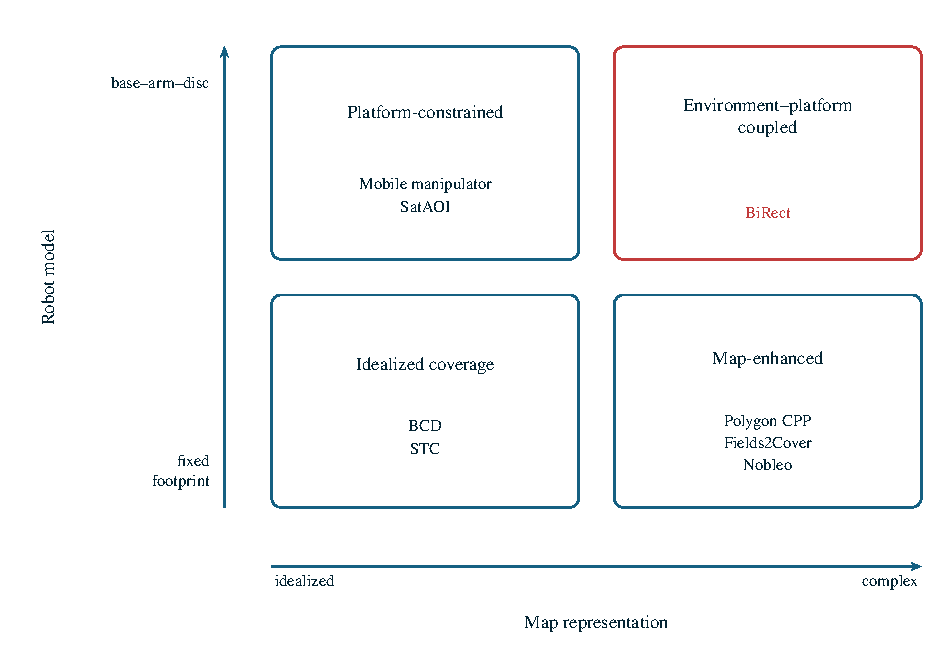
\includegraphics[width=0.88\linewidth]{figures/figure_cpp_class_quadrant.pdf}}}\\[0.25em]
{\color{blue}\scriptsize 新增}
% ===FIGNEW END figure_cpp_class_quadrant.png===
  \caption{\DIFaddFL{Four capability classes arranged by map representation and robot model.}}
  \label{fig:cpp-classes}
\end{figure}\marginpar{\scriptsize [25] 用已有四类关系新画坐标示意图，未使用实验数据。}
\DIFaddend 

The first class comprises classical coverage algorithms that express the core coverage idea clearly but generally close the problem only for idealized maps and simplified robot models. Representative methods include Boustrophedon Cellular Decomposition (BCD) and Spanning Tree Coverage (STC). BCD \DIFdelbegin \DIFdel{partitions an area where scan-line connectivity changes and }\DIFdelend \DIFaddbegin \DIFadd{scans the free space and ends the current cell when the number of free intervals on the scan line changes, then }\marginpar{\scriptsize [20] 为前三类各补一句基本思路，没有增加算法。}\DIFaddend generates back-and-forth sweeps \DIFdelbegin \DIFdel{within each cell \mbox{%DIFAUXCMD
\cite{choset1998}}\hskip0pt%DIFAUXCMD
; STC }\DIFdelend \DIFaddbegin \DIFadd{inside the cell \mbox{%DIFAUXCMD
\cite{choset1998}}\hskip0pt%DIFAUXCMD
. STC coarsens the free space into a grid, }\DIFaddend builds a spanning tree \DIFdelbegin \DIFdel{over a free-space grid and systematically traverses its }\DIFdelend \DIFaddbegin \DIFadd{on that grid, and walks the fine cells around the tree }\DIFaddend boundary \cite{gabriely2001}. These methods establish the respective roles of cellular decomposition and graph traversal\DIFdelbegin \DIFdel{, but their coverage primitive is typically a point robot, disc robot, or fixed-width tool. Applied directly to swing-arm troweling, they cannot distinguish the relative poses }\DIFdelend \DIFaddbegin \DIFadd{. They do not represent the relative position }\marginpar{\scriptsize [21] 将第一类局限改为不能表示 base 与 disc 的相对位置和臂角。}\DIFaddend of the base \DIFdelbegin \DIFdel{, arm, and disc or represent how arm-angle changes affect the instantaneous footprint and collision risk}\DIFdelend \DIFaddbegin \DIFadd{and the disc, nor the change of the arm angle $\phi$, and are therefore difficult to apply to swing-arm troweling, on which the disc moves relative to the base}\DIFaddend .

The second class \DIFdelbegin \DIFdel{offers stronger complex-map representation and includes reproducible open-source frameworks, but still models }\marginpar{\scriptsize [22] 在类定义中删去 open-source，固定足迹仍留在定义里。}\DIFdelend \DIFaddbegin \DIFadd{can represent complex maps, but }\DIFaddend the robot and tool \DIFdelbegin \DIFdel{mainly through }\DIFdelend \DIFaddbegin \DIFadd{are still modeled mainly by }\DIFaddend a fixed footprint. \DIFdelbegin \DIFdel{Examples }\DIFdelend \DIFaddbegin \DIFadd{It first represents a map with holes, non-convex boundaries, or obstacles, then covers that map with fixed-width strips, orders the regions, and connects them by collision-free turns. Reproducible examples }\DIFaddend include ETH Zurich's \texttt{polygon\_coverage\_planning} \DIFaddbegin \DIFadd{\mbox{%DIFAUXCMD
\cite{bahnemann2021,polygoncoverage}}\hskip0pt%DIFAUXCMD
}\DIFaddend , Fields2Cover for agricultural vehicles \DIFaddbegin \DIFadd{\mbox{%DIFAUXCMD
\cite{mier2023,fields2cover}}\hskip0pt%DIFAUXCMD
}\DIFaddend , and the Nobleo Full Coverage Path Planner for ROS occupancy grids \DIFdelbegin \DIFdel{. The first }\DIFdelend \DIFaddbegin \DIFadd{\mbox{%DIFAUXCMD
\cite{nobleo}}\hskip0pt%DIFAUXCMD
. }\texttt{\DIFadd{polygon\_coverage\_planning}} \DIFaddend handles general polygons with holes, uses BCD or trapezoidal decomposition to generate cells, constructs multiple sweep candidates for each cell, and performs global selection and collision-free transfer through an Equality Generalized Traveling Salesman Problem and a visibility graph\DIFdelbegin \DIFdel{\mbox{%DIFAUXCMD
\cite{bahnemann2021,polygoncoverage}}\hskip0pt%DIFAUXCMD
}\DIFdelend . Fields2Cover supports non-convex fields, obstacles, headlands, swaths, \DIFaddbegin \DIFadd{and }\DIFaddend route ordering, and \DIFaddbegin \DIFadd{connects swaths by }\DIFaddend curvature-constrained Dubins or Reeds--Shepp connections \cite{mier2023,fields2cover}. Nobleo's planner implements a Backtracking Spiral Algorithm/Spiral-STC-type method \DIFaddbegin \DIFadd{\mbox{%DIFAUXCMD
\cite{nobleo} }\hskip0pt%DIFAUXCMD
}\DIFaddend on a ROS occupancy grid and permits separate robot and tool radii\DIFdelbegin \DIFdel{\mbox{%DIFAUXCMD
\cite{nobleo}}\hskip0pt%DIFAUXCMD
}\DIFdelend . These frameworks show that complex boundaries, obstacles, and engineering interfaces can be addressed systematically. Their tool width, implement width, or tool disc nevertheless remains essentially fixed relative to the base and cannot represent the time-varying sweep caused by continuous changes in $\phi$.

The third class \DIFdelbegin \DIFdel{emphasizes robot motion constraints, reachability, and collision relationships, but usually does not target complete coverage of a complex two-dimensional floor}\DIFdelend \DIFaddbegin \DIFadd{retains, during planning, the minimum turning radius, the reachable range of the arm, and component collisions, while its scenes are mostly regular sites, local surfaces, or three-dimensional objects}\DIFaddend . It includes the nonholonomic vehicle connections in Fields2Cover and mobile-manipulator surface-coverage methods for tasks such as spray disinfection. Fields2Cover incorporates minimum turning radius and vehicle kinematics \cite{mier2023,fields2cover}, but targets agricultural swaths with a fixed implement width. Mobile-manipulator studies explicitly handle the base, arm, end tool, reachability, and occlusion. For example, spray-based surface disinfection can generate end-effector paths from three-dimensional surfaces and jointly select base positions and arm motions \cite{thakar2022}. Such methods describe how a robot executes a task in greater detail, but generally target regular sites, agricultural strips, or three-dimensional object surfaces rather than jointly performing obstacle handling, area decomposition, global traversal, and continuous ground-coverage evaluation on a known two-dimensional construction map.

\DIFaddbegin \DIFadd{Swing-arm troweling therefore requires the fourth class shown in Fig.~\ref{fig:cpp-classes}. Walls, columns, reserved openings, and narrow corridors divide the floor into irregular regions with complex connectivity, which the planner must represent and visit continuously. Meanwhile, the disc position is jointly determined by base motion and active swing-arm motion; coverage and collision status vary continuously with base heading and arm angle and cannot be approximated by a fixed footprint. A complete, continuous, and executable route therefore requires the construction map and the coordinated base--swing-arm--disc behavior to be represented in the same planning model.
}\marginpar{\scriptsize [19] 把第四类需求段挪到三类介绍之后。}

\DIFaddend Research has thus advanced in both complex-map representation and robot-behavior modeling, but the two have not yet been unified\DIFaddbegin \DIFadd{, especially }\marginpar{\scriptsize [24] 在 unified 与 for 之间插入逗号和 especially。}\DIFaddend for swing-arm floor coverage. CPP frameworks with strong map support usually assume a fixed tool footprint and cannot describe the dynamic coverage created by a rotating arm. Methods that model vehicle kinematics, manipulator reachability, and component collisions in detail generally focus on regular sites, local operations, or three-dimensional surfaces and do not fully decompose and continuously traverse a complex two-dimensional construction map. SatAOI considers both an obstacle map and the geometry of the base, arm, and disc, but stops at delimiting the workable area and does not produce a visitation order, transfer route, or coordinated coverage trajectory within each region \cite{lin2025}. The central gap is therefore a swing-arm troweling CPP method that combines complex-map processing with high-fidelity robot-behavior modeling and generates a complete, continuous, executable route directly from the construction map.

Table~\ref{tab:cpp-comparison} compares representative approaches along these two dimensions\marginpar{\scriptsize [26] 把表中地图与工具合并的那一列拆成地图表示和机器人模型两列。}. Work spanning more than one class is placed according to its principal contribution: Fields2Cover is treated as map-enhanced and SatAOI as platform-constrained. The stated limitations concern direct application\marginpar{\scriptsize [27] 将最后一列改为 Pros and cons，并用原有格子拆出优点和局限。} to a mobile base with an active arm and circular disc; they are not general judgments of the methods or software.

\DIFdelbegin %DIFDELCMD < \begin{longtable}{@{}>{\raggedright\arraybackslash}p{0.16\linewidth}>{\raggedright\arraybackslash}p{0.18\linewidth}>{\raggedright\arraybackslash}p{0.21\linewidth}>{\raggedright\arraybackslash}p{0.36\linewidth}@{}}
%DIFDELCMD < %%%
\DIFdelend \DIFaddbegin \begin{longtable}{@{}>{\raggedright\arraybackslash}p{0.13\linewidth}>{\raggedright\arraybackslash}p{0.15\linewidth}>{\raggedright\arraybackslash}p{0.14\linewidth}>{\raggedright\arraybackslash}p{0.16\linewidth}>{\raggedright\arraybackslash}p{0.30\linewidth}@{}}
\DIFaddend \caption{Representative CPP methods and their applicability to swing-arm troweling.}\label{tab:cpp-comparison}\\
\toprule
Category & Representative method & \DIFdelbegin \DIFdel{Map and tool model}\DIFdelend \DIFaddbegin \DIFadd{Map representation }& \DIFadd{Robot model}\DIFaddend & \DIFdelbegin \DIFdel{Relevance to swing-arm troweling }\DIFdelend \DIFaddbegin \DIFadd{Pros and cons }\DIFaddend \\
\midrule
\endfirsthead
\toprule
Category & Representative method & \DIFdelbegin \DIFdel{Map and tool model}\DIFdelend \DIFaddbegin \DIFadd{Map representation }& \DIFadd{Robot model}\DIFaddend & \DIFdelbegin \DIFdel{Relevance to swing-arm troweling }\DIFdelend \DIFaddbegin \DIFadd{Pros and cons }\DIFaddend \\
\midrule
\endhead
Idealized coverage & BCD \cite{choset1998} & Cellular decomposition \DIFdelbegin \DIFdel{; fixed }\DIFdelend \DIFaddbegin & \DIFadd{Fixed }\DIFaddend footprint & \DIFaddbegin \DIFadd{$\checkmark$ }\DIFaddend Organizes back-and-forth sweeps within cells\DIFdelbegin \DIFdel{, but does not model }\DIFdelend \DIFaddbegin \DIFadd{.}\newline \DIFadd{$\times$ Does not represent }\DIFaddend an active arm or \DIFdelbegin \DIFdel{its }\DIFdelend continuous sweep. \\
Idealized coverage & STC \cite{gabriely2001} & Grid spanning tree \DIFdelbegin \DIFdel{; simplified }\DIFdelend \DIFaddbegin & \DIFadd{Point or disc }\DIFaddend robot & \DIFaddbegin \DIFadd{$\checkmark$ }\DIFaddend Systematically traverses a grid\DIFdelbegin \DIFdel{, but cannot exploit }\DIFdelend \DIFaddbegin \DIFadd{.}\newline \DIFadd{$\times$ Cannot use }\DIFaddend the time-varying \DIFdelbegin \DIFdel{tool }\DIFdelend \DIFaddbegin \DIFadd{disc }\DIFaddend position created by arm motion. \\
Map-enhanced & Polygon CPP \cite{bahnemann2021,polygoncoverage} & Polygon with holes \DIFdelbegin \DIFdel{; fixed tool }\DIFdelend & \DIFdelbegin \DIFdel{Provides alternative sweeps }\DIFdelend \DIFaddbegin \DIFadd{Fixed footprint }& \DIFadd{$\checkmark$ Provides alternative strips }\DIFaddend and obstacle-avoiding transfers\DIFdelbegin \DIFdel{, but does }\DIFdelend \DIFaddbegin \DIFadd{.}\newline \DIFadd{$\times$ Does }\DIFaddend not represent the arm's instantaneous \DIFdelbegin \DIFdel{footprint}\DIFdelend \DIFaddbegin \DIFadd{disc position}\DIFaddend . \\
Map-enhanced & Fields2Cover \cite{mier2023,fields2cover} & Non-convex field \DIFdelbegin \DIFdel{; fixed-width implement }\DIFdelend & \DIFaddbegin \DIFadd{Fixed footprint }& \DIFadd{$\checkmark$ }\DIFaddend Includes swaths, route ordering, and curvature-constrained connections\DIFdelbegin \DIFdel{; the fixed implement model }\DIFdelend \DIFaddbegin \DIFadd{.}\newline \DIFadd{$\times$ The fixed footprint }\DIFaddend omits arm motion. \\
Map-enhanced & Nobleo FCPP \cite{nobleo} & Occupancy grid \DIFdelbegin \DIFdel{; fixed tool disc }\DIFdelend & \DIFaddbegin \DIFadd{Fixed footprint }& \DIFadd{$\checkmark$ }\DIFaddend Integrates grid coverage with a navigation stack\DIFdelbegin \DIFdel{, but does }\DIFdelend \DIFaddbegin \DIFadd{.}\newline \DIFadd{$\times$ Does }\DIFaddend not coordinate arm angle, arm \DIFdelbegin \DIFdel{speed}\DIFdelend \DIFaddbegin \DIFadd{angular velocity}\DIFaddend , and base speed. \\
Platform-constrained & Mobile-manipulator surface coverage \cite{thakar2022} & Three-dimensional surface \DIFdelbegin \DIFdel{; mobile }\DIFdelend \DIFaddbegin & \DIFadd{Mobile }\DIFaddend manipulator & \DIFaddbegin \DIFadd{$\checkmark$ }\DIFaddend Jointly plans base placement and end-tool motion\DIFdelbegin \DIFdel{, but does }\DIFdelend \DIFaddbegin \DIFadd{.}\newline \DIFadd{$\times$ Does }\DIFaddend not completely traverse a complex two-dimensional floor. \\
Platform-constrained & SatAOI \cite{lin2025} & Construction obstacle map \DIFdelbegin \DIFdel{; base}\DIFdelend \DIFaddbegin & \DIFadd{Base}\DIFaddend , arm, and disc & \DIFaddbegin \DIFadd{$\checkmark$ }\DIFaddend Determines workable regions and connectivity\DIFdelbegin \DIFdel{, but does }\DIFdelend \DIFaddbegin \DIFadd{.}\newline \DIFadd{$\times$ Does }\DIFaddend not generate a visitation order or continuous coverage trajectory. \\
Proposed method & \DIFdelbegin \DIFdel{Hierarchical swing-arm CPP }\DIFdelend \DIFaddbegin \DIFadd{BiRect }\DIFaddend & Two-dimensional obstacle map \DIFdelbegin \DIFdel{; }\DIFdelend \DIFaddbegin & \DIFadd{Swing arm with a }\DIFaddend time-varying disc \DIFdelbegin \DIFdel{sweep }\DIFdelend & \DIFaddbegin \DIFadd{$\checkmark$ }\DIFaddend Links rectangular decomposition, visitation, local swinging, and trajectory evaluation\DIFdelbegin \DIFdel{; currently }\DIFdelend \DIFaddbegin \DIFadd{.}\newline \DIFadd{$\times$ Currently }\DIFaddend assumes a static map and uses heuristic search. \\
\bottomrule
\end{longtable}

\subsection{Summary and Research Gap}

Prior work provides several capabilities needed here, but has not solved complex-map coverage within one unified task. BCD \DIFdelbegin \DIFdel{, STC, and related frameworks }\marginpar{\scriptsize [23] 把引用贴到算法名称上，不再挂在 frameworks 上。}\DIFdelend \DIFaddbegin \DIFadd{\mbox{%DIFAUXCMD
\cite{choset1998} }\hskip0pt%DIFAUXCMD
and STC \mbox{%DIFAUXCMD
\cite{gabriely2001} }\hskip0pt%DIFAUXCMD
}\DIFaddend can represent two-dimensional free spaces \DIFdelbegin \DIFdel{containing holes, non-convex boundaries, or multiple obstacles }\DIFdelend and can decompose regions \DIFdelbegin \DIFdel{, generate swaths, }\DIFdelend or traverse grids. \DIFaddbegin \DIFadd{Decomposition and swath generation on regions with holes or non-convex boundaries are given in \mbox{%DIFAUXCMD
\cite{bahnemann2021,polygoncoverage}}\hskip0pt%DIFAUXCMD
, and grid traversal in \mbox{%DIFAUXCMD
\cite{nobleo}}\hskip0pt%DIFAUXCMD
. }\marginpar{\scriptsize [28] 把研究缺口开头的引用按半句拆开。}\DIFaddend With a tool fixed to the base, they can arrange adjacent sweeps according to a prescribed width. Fields2Cover additionally generates turns and \DIFaddbegin \DIFadd{curvature-constrained }\DIFaddend connections for vehicles whose direction and minimum turning radius prevent arbitrary lateral motion \DIFaddbegin \DIFadd{\mbox{%DIFAUXCMD
\cite{mier2023,fields2cover}}\hskip0pt%DIFAUXCMD
}\DIFaddend . Mobile-manipulator research addresses end-tool reachability and collision relationships \DIFaddbegin \DIFadd{\mbox{%DIFAUXCMD
\cite{thakar2022}}\hskip0pt%DIFAUXCMD
}\DIFaddend , while SatAOI uses the geometry among the base, \DIFaddbegin \DIFadd{swing }\DIFaddend arm, disc, and obstacles to delimit regions the robot can enter and the disc can treat \DIFdelbegin \DIFdel{\mbox{%DIFAUXCMD
\cite{lin2025,choset1998,gabriely2001,bahnemann2021,polygoncoverage,mier2023,fields2cover,nobleo,thakar2022}}\hskip0pt%DIFAUXCMD
}\DIFdelend \DIFaddbegin \DIFadd{\mbox{%DIFAUXCMD
\cite{lin2025}}\hskip0pt%DIFAUXCMD
}\DIFaddend . These abilities remain distributed across different task models and applications: complex-map CPP usually assumes a fixed footprint, detailed robot models are commonly used for local or regular workspaces, and SatAOI terminates at workable-area delimitation. For the specific objective of generating a complete executable route for a swing-arm troweling robot in a known, complex, two-dimensional construction map, three coupled gaps remain\marginpar{\scriptsize [29] 使三条研究缺口各留主题句，不再重讲前一小节。}.

First, existing CPP methods do not model active \DIFaddbegin \DIFadd{swing-}\DIFaddend arm behavior sufficiently to plan the actual coverage of the \DIFdelbegin \DIFdel{end disc. In conventional CPP , }\DIFdelend \DIFaddbegin \DIFadd{disc: in conventional CPP }\DIFaddend the tool is fixed \DIFdelbegin \DIFdel{relative }\DIFdelend to the base, so determining the base route also determines \DIFdelbegin \DIFdel{tool position and coverage. For a swing-arm robot, }\DIFdelend \DIFaddbegin \DIFadd{coverage. At }\DIFaddend the same base position and heading\DIFdelbegin \DIFdel{admit multiple arm poses and therefore different disc positions, swept regions, and }\DIFdelend \DIFaddbegin \DIFadd{, a different arm angle places the disc center on an arc whose radius is the arm length, and the }\marginpar{\scriptsize [30] 将同一基座位姿下的多个臂角改写成盘心圆弧和碰撞两句。}\DIFaddend whole-robot collision \DIFdelbegin \DIFdel{states. Approximating this behavior by the maximum arm reach or an enlarged fixed width confuses geometric reachability in one pose with coverage throughout continuous motion and cannot test the combined collision state of the base, arm, and disc during execution. SatAOI models the geometry and collision relationships among these components but uses them primarily to determine workable positions rather than continuous coverage motion\mbox{%DIFAUXCMD
\cite{lin2025}}\hskip0pt%DIFAUXCMD
.
The present method therefore preserves the relationship among base motion, arm rotation, and the circular-disc sweep during both trajectory generation and evaluation.
}\marginpar{\scriptsize [31] 删去 SatAOI 主要用于可作业位置的两句。}\DIFdelend \DIFaddbegin \DIFadd{state differs as well. Maximum arm reach, or a widened strip, only shows that some pose can reach a location; it is not coverage during continuous motion.
}\DIFaddend 

Second, complex-map decomposition and local swing motion have not been integrated into a computationally practical planning chain. \DIFdelbegin \DIFdel{Existing complex-map CPP frameworks handle polygons with holes, non-convex boundaries, or occupancy grids and produce partitions and global routes, but their local coverage actions typically rely on a fixed tool footprint \mbox{%DIFAUXCMD
\cite{bahnemann2021,polygoncoverage,mier2023,fields2cover,nobleo}}\hskip0pt%DIFAUXCMD
. Mobile-manipulator methods plan local base and end-tool motions in detail but generally do not decompose and continuously traverse an entire complex two-dimensional floor \mbox{%DIFAUXCMD
\cite{thakar2022}}\hskip0pt%DIFAUXCMD
. SatAOI identifies workable regions and their connectivity but does not proceed to visitation ordering, inter-region transfers, or coordinated intra-region coverage \mbox{%DIFAUXCMD
\cite{lin2025}}\hskip0pt%DIFAUXCMD
. Directly enumerating decompositions, visitation orders, and arm trajectories together would cause the number of combinations to grow with the obstacles and work units, undermining computational efficiency and field practicality. The proposed method instead organizes complex-space decomposition, }\marginpar{\scriptsize [32] 在第二缺口删去句末复述固定足迹的那一句。}\DIFdelend \DIFaddbegin \DIFadd{SatAOI stops at the workable area; this paper uses a hierarchical heuristic to join }\marginpar{\scriptsize [33] 使第二缺口只保留 SatAOI 停在可作业区域的一句。}\DIFaddend region connectivity, \DIFdelbegin \DIFdel{global visitation }\DIFdelend \DIFaddbegin \DIFadd{visitation order}\DIFaddend , and coordinated \DIFdelbegin \DIFdel{base--arm coverage as a hierarchical heuristic pipeline that converts map-level decisions into continuous work routes while controlling the candidate-search space}\DIFdelend \DIFaddbegin \DIFadd{base--swing-arm coverage inside each region into one computable chain}\DIFaddend .

Third, a static reachability envelope does not guarantee complete coverage during dynamic execution, and prior work does not explicitly model \DIFdelbegin \DIFdel{the matching between }\DIFdelend \DIFaddbegin \DIFadd{base--arm velocity coupling, the coordination of }\DIFaddend base linear velocity and arm angular velocity. Maximum arm reach indicates only which locations the disc can touch in some poses. \DIFdelbegin \DIFdel{During continuous base advance and periodic arm swinging, coverage continuity depends on the number of sweeps per unit distance. If }\DIFdelend \DIFaddbegin \DIFadd{While the base advances continuously and the swing arm swings periodically, }\DIFaddend the \DIFaddbegin \DIFadd{longitudinal spacing between consecutive sweeps is determined by base speed and arm angular velocity; if the }\marginpar{\scriptsize [35] 把车速与摆臂角速度决定扫掠间距的两句并成一句。}\DIFaddend base is too fast or the \DIFaddbegin \DIFadd{swing }\DIFaddend arm too slow, \DIFdelbegin \DIFdel{the longitudinal spacing between consecutive sweeps increases, leaving untreated gaps }\DIFdelend \DIFaddbegin \DIFadd{untreated gaps remain }\DIFaddend even when the target lies inside the \DIFdelbegin \DIFdel{geometric reach envelope . Evaluation based only on that envelope or on an untimed geometric path therefore mistakes ``reachable'' for ``covered.'' This paper incorporates the relationship between base and arm velocities into the coverage analysis and calculates coverage ratio and task time from the area actually swept during continuous motion, exposing the joint effect of speed parameters on gaps and time cost.
}\DIFdelend \DIFaddbegin \DIFadd{static reachability envelope defined above, so being reachable is not the same as being covered.
}\DIFaddend 

\DIFdelbegin \DIFdel{In summary, the core research gap is the absence of an end-to-end CPP method that, in a known two-dimensional construction environment with dense obstacles, connects active-arm behavior modeling, global--local coverage planning for a complex map, and continuous swept-area evaluation under coupled base and arm velocities.
This work aims to complete the planning chain from a construction map and swing-arm robot model to a complete, continuous, executable coverage trajectory, with final coverage quality determined by the disc sweep under the specified velocity relationship.
}\marginpar{\scriptsize [36] 删去把速度分析写入覆盖的一段和文末缺口总结。}%DIFDELCMD < 

%DIFDELCMD < %%%
\DIFdelend \section{Methodology}
\label{sec:methodology}

This study addresses the planning problem that maps a known, static, two-dimensional obstacle environment to a complete coverage trajectory for a swing-arm troweling robot. Walls, columns, and openings divide a construction floor into a free space with complex geometry and connectivity, while the disc position and footprint are jointly determined by the base pose and arm angle. The planner must therefore organize global visitation of the free space and convert coverage of each region into continuous, coordinated base--arm motion. Subject to obstacle-avoidance, geometric, and motion constraints, the objectives are to increase effective coverage of the target floor and reduce both trajectory execution time and planning time. The number of rectangles, their overlap, and the number of inter-rectangle transfers are intermediate measures only; they are converted into proxy costs for polynomial-time heuristics at the respective planning levels.

\subsection{Overall Planning Pipeline}

\DIFdelbegin \DIFdel{The proposed hierarchy follows four stages: region representation, graph visitation, local execution, and coverage evaluation}\DIFdelend \DIFaddbegin \DIFadd{BiRect proceeds in four stages, and the output of each stage is the input of the next}\marginpar{\scriptsize [43] 把流程开头改成四段数据交接，未提前定义后文符号。}\DIFaddend . Figure~\ref{fig:pipeline} summarizes the \DIFdelbegin \DIFdel{data flow. The inputs comprise a calibrated binary work map \mbox{$M$} with physical pixel size \mbox{$s_p$}, an initial robot state \mbox{$q_0$}, geometric and motion parameters \mbox{$\Theta_R$} for the base--arm--disc mechanism, and planning configuration \mbox{$\Psi_P$}. These quantities are defined formally in Section~\mbox{\ref{sec:formulation}}; the present subsection explains how they are progressively transformed into an executable trajectory and coverage measures.
}\marginpar{\scriptsize [37] 将 data flow 改为 workflow。}%DIFDELCMD < 

%DIFDELCMD < \begin{figure}[htbp]
%DIFDELCMD <   \centering
%DIFDELCMD <   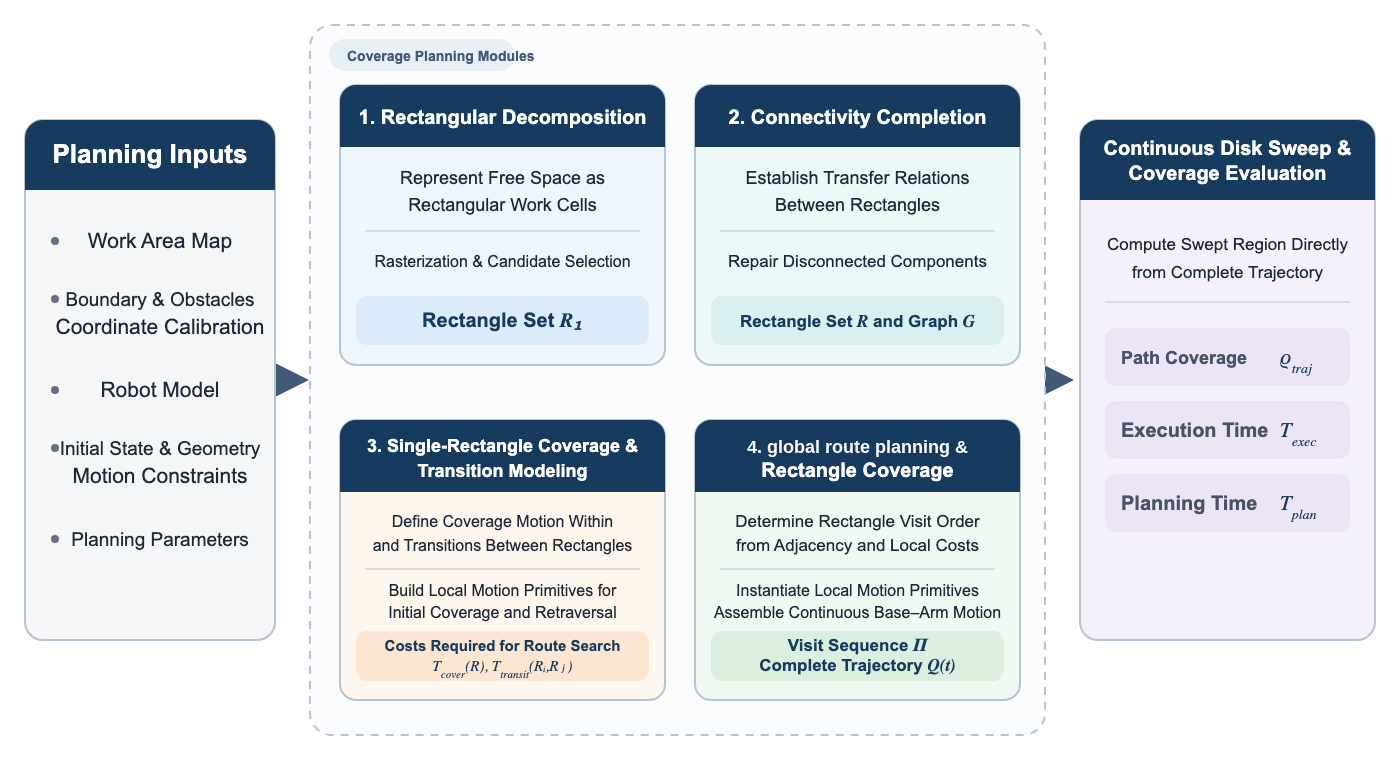
\includegraphics[width=0.98\linewidth]{pipeline_overall_improved_en.png}
%DIFDELCMD <   %%%
%DIFDELCMD < \caption{%
{%DIFAUXCMD
\DIFdelFL{Coverage-planning framework and principal data flow. The inputs on the left are the work map, coordinate calibration, robot model, initial state, and planning parameters. The four central modules successively produce an initial rectangle set \mbox{$\mathcal R_1$}, a final rectangle set \mbox{$\mathcal R$} with adjacency graph \mbox{$G$}, entry- and exit-constrained local motion primitives with time costs, and a visitation sequence \mbox{$\Pi$} with complete trajectory \mbox{$q(t)$}. Continuous disc sweeping then yields coverage ratios, execution time, and planning time.}}
  %DIFAUXCMD
%DIFDELCMD < \label{fig:pipeline}
%DIFDELCMD < \end{figure}
%DIFDELCMD < 

%DIFDELCMD < %%%
\DIFdel{The rectangular-decomposition module first generates candidate rectangles on a conservative planning grid and selects suitable work units according to newly covered area, rectangle count, and overlap, producing the initial set \mbox{$\mathcal R_1$}. The connectivity-completion module creates geometric adjacency candidates, removes relationships that fail a base--arm transfer check, and inserts bridging rectangles when needed. Its output is a final rectangle set \mbox{$\mathcal R$} and }\DIFdelend \DIFaddbegin \DIFadd{workflow. To improve the efficiency of searching a complex free space, rectangular decomposition gathers that space into a small number of bidirectional rectangular candidates. Connectivity completion outputs a }\marginpar{\scriptsize [40] 在矩形分解前补上提高复杂自由空间搜索效率。}\DIFaddend feasible adjacency graph $G$\DIFdelbegin \DIFdel{. An edge in \mbox{$G$} therefore means not only that two rectangles touch geometrically, but also that at least one local transfer satisfies }\DIFdelend \DIFaddbegin \DIFadd{, whose edges mean that a base--swing-arm transfer satisfying }\DIFaddend the geometric and velocity constraints \DIFdelbegin \DIFdel{in Eqs.~\mbox{\eqref{eq:geometric-feasibility}} and \mbox{\eqref{eq:velocity-limits}}.
}%DIFDELCMD < 

%DIFDELCMD < %%%
\DIFdel{For every rectangle, the local-modeling module constructs two primitive types. A first visit uses a coverage primitive, whereas a repeated visit uses a transit primitive. Their durations depend on the entry and exit states and are denoted by \mbox{$T_{\mathrm{cover}}(R;q^{\mathrm{in}},q^{\mathrm{out}})$} and \mbox{$T_{\mathrm{transit}}(R;q^{\mathrm{in}},q^{\mathrm{out}})$}, respectively. These costs, together with the transfer costs on graph edges, enter the global route search. After the visitation sequence \mbox{$\Pi$} has been selected, the same primitives are instantiated as first-visit or repeated-visit motions and concatenated into the complete trajectory. The local motion model thus supports both visitation ordering and final trajectory generation.
}%DIFDELCMD < 

%DIFDELCMD < %%%
\DIFdel{Starting from \mbox{$q_0$}, the global module generates a }\DIFdelend \DIFaddbegin \DIFadd{exists, not merely that two rectangles touch. Then each rectangle supplies the time of a first coverage visit and of a repeated transit visit, and these times are used as the costs of global route planning. The global stage obtains a visitation }\marginpar{\scriptsize [41] 将局部运动并回流程，并用 Then 接上。}\marginpar{\scriptsize [42] 将 enter 改为 are used as the costs of。}\DIFaddend sequence on $G$ \DIFdelbegin \DIFdel{that permits repeated transit visits and connects adjacent primitive endpoints, yielding a continuous trajectory\mbox{$q(t)$} with timing and work-state labels. The evaluation module recovers the disc-center path from \mbox{$q(t)$} and computes effective-work coverage \mbox{$\rho_{\mathrm{work}}$}, full-trajectory coverage \mbox{$\rho_{\mathrm{traj}}$}, and execution time \mbox{$T_{\mathrm{exec}}$}. The wall-clock time from conservative-grid generation through trajectory evaluation is }\DIFdelend \DIFaddbegin \DIFadd{and joins it into a trajectory; evaluation reads only this trajectory and returns the coverage ratios and the execution time, while }\DIFaddend $T_{\mathrm{plan}}$ \DIFdelbegin \DIFdel{. The following subsections define the inputs, states, and metrics, then describe each module and the continuous swept-area evaluation}\DIFdelend \DIFaddbegin \DIFadd{is the computation time of the whole workflow and is not used as a search cost}\DIFaddend .

\DIFaddbegin \begin{figure}[htbp]
  \centering
  % ===FIGPAIR pipeline_overall_improved_en.png===
\par\noindent\begin{minipage}[t]{0.48\linewidth}\centering
{\setlength{\fboxsep}{1.2pt}\setlength{\fboxrule}{1.1pt}%
\fcolorbox{red}{white}{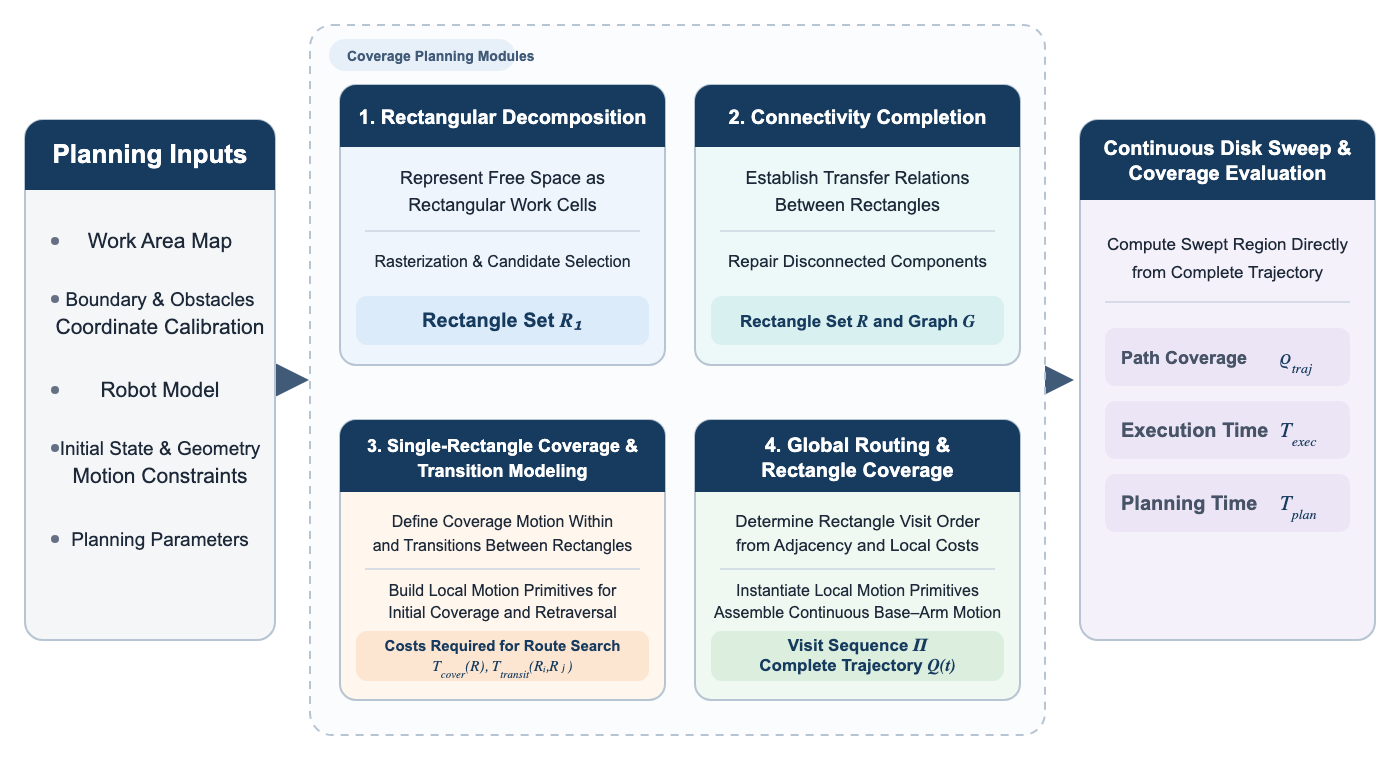
\includegraphics[width=\dimexpr\linewidth-2\fboxsep-2\fboxrule\relax]{old_figs/pipeline_overall_improved_en.png}}}\\[0.25em]
{\color{red}\scriptsize 修改前}
\end{minipage}\hfill
\begin{minipage}[t]{0.48\linewidth}\centering
{\setlength{\fboxsep}{1.2pt}\setlength{\fboxrule}{1.1pt}%
\fcolorbox{blue}{white}{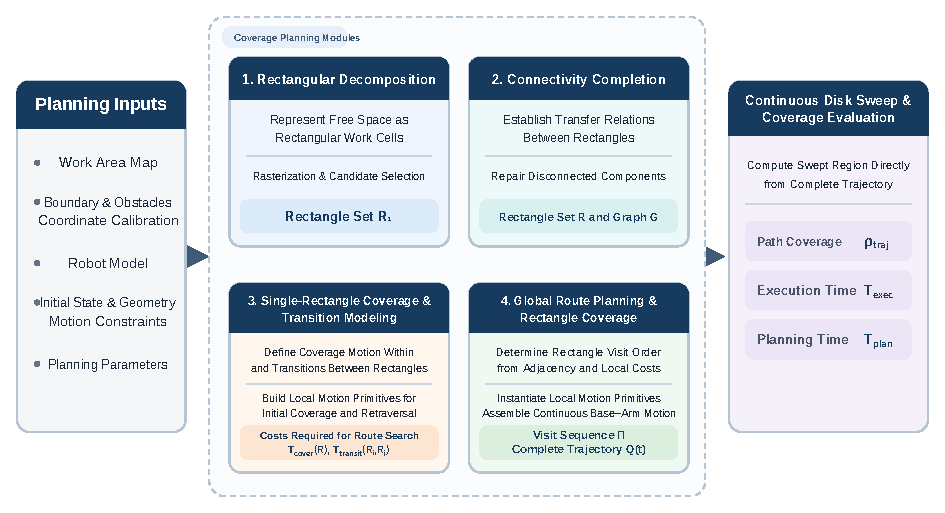
\includegraphics[width=\dimexpr\linewidth-2\fboxsep-2\fboxrule\relax]{figures/pipeline_overall_improved_en.pdf}}}\\[0.25em]
{\color{blue}\scriptsize 修改后}
\end{minipage}\par
% ===FIGPAIR END pipeline_overall_improved_en.png===
  \caption{\DIFaddFL{Workflow of BiRect.}}
  \label{fig:pipeline}
\end{figure}\marginpar{\scriptsize [38] 统一为 global route planning，并改了流程图中的 Global Routing 标签。}\marginpar{\scriptsize [39] 把总流程图的图注收成一句，且未改图内像素。}

\DIFaddend \subsection{Problem Formulation and Notation}
\label{sec:formulation}

\subsubsection{From a Construction Scene to Planning Inputs}
\DIFaddbegin \label{sec:scene-inputs}
\DIFaddend 

The required scene information is first extracted from a CAD/BIM model, site-survey data, or localization and mapping output. For a floor to be troweled, a world-coordinate plane $\mathcal F_W$ coincident with the work surface is selected, and the boundary of the current task is specified in that plane. Walls, columns, equipment foundations, embedded components, reserved openings, and areas outside the work boundary are marked as unavailable. The remaining floor inside the boundary on which the disc may operate becomes the target work region. \DIFdelbegin \DIFdel{To account for localization error, map error, or additional clearance, unavailable-region contours can be dilated by a margin \mbox{$\delta_{\mathrm{map}}$} before rasterization. }\DIFdelend The classified plane is then rasterized and geometrically calibrated to produce a physically scaled binary work map \DIFaddbegin \DIFadd{$M$}\DIFaddend , which is the direct map input to CPP.

\DIFdelbegin \DIFdel{Discretization converts heterogeneous geometry from CAD/BIM, field measurement, and mapping into spatial cells at a common resolution. This gives rectangle generation, adjacency testing, collision checking, and coverage calculation a consistent computational basis. }\marginpar{\scriptsize [45] 与相邻三条一起压缩重复段落，没有另加句子。}\DIFdelend At a resolution of $s_p$~m/pixel, \DIFdelbegin \DIFdel{the plane becomes a binary map \mbox{$M$}: white pixels are obstacle-free target pixels included in the coverage task, whereas black pixels represent walls, columns, openings, out-of-bound areas, and areas excluded by the safety margin. In }\DIFdelend \DIFaddbegin \DIFadd{blue pixels in }\marginpar{\scriptsize [44] 将场景到二值图的叙述压成一条。}\DIFaddend result and evaluation images \DIFdelbegin \DIFdel{, blue pixels }\DIFdelend denote portions of the target region already swept by the disc. Blue is an overlay on $M$, not a third input-map class. A rigid transform $T_{WM}$ calibrates image coordinates to world coordinates, so every pixel corresponds to a physical location in metres.

\DIFdelbegin \DIFdel{The conversion from planar geometry to the binary map follows uniform labeling and conservative discretization. Regardless of boundary shape, all workable and unavailable regions are projected onto the same plane and classified at one resolution as free or occupied cells. Cells on an obstacle boundary or with ambiguous membership are }\DIFdelend \DIFaddbegin \DIFadd{Unavailable regions are first enlarged by the safety margin $\delta_{\mathrm{map}}$ and then rasterized, and every boundary cell or cell of ambiguous membership is }\marginpar{\scriptsize [46] 把安全边距膨胀和边界单元判为不可用合成一条保守规则。}\DIFaddend treated as unavailable\DIFdelbegin \DIFdel{to avoid misclassifying obstacle space as workable floor. Straight walls and rectangular foundations map directly to contiguous black cells. }\DIFdelend \DIFaddbegin \DIFadd{. }\DIFaddend Circular columns, curved boundaries, and openings \DIFdelbegin \DIFdel{are approximated by }\DIFdelend \DIFaddbegin \DIFadd{become }\DIFaddend staircase boundaries at the selected resolution\DIFdelbegin \DIFdel{, optionally enlarged by the safety margin. In regions with irregular boundaries or dense obstacles, the occupancy map preserves the overall shape and connectivity; subsequent rectangle generation, hole filling, and connectivity completion handle them uniformly. The conversion therefore does not require a separate decomposition rule for every geometric shape. Its approximation accuracy is governed jointly by map resolution and safety margin}\DIFdelend . \DIFaddbegin \DIFadd{Straight walls and rectangular foundations map to contiguous occupied cells.
}\marginpar{\scriptsize [47] 使该段只保留保守栅格化的操作规则。}\DIFaddend 

\begin{figure}[htbp]
  \centering
  % ===FIGPAIR figure_3_geometric_to_binary_raster.png===
\par\noindent\begin{minipage}[t]{0.48\linewidth}\centering
{\setlength{\fboxsep}{1.2pt}\setlength{\fboxrule}{1.1pt}%
\fcolorbox{red}{white}{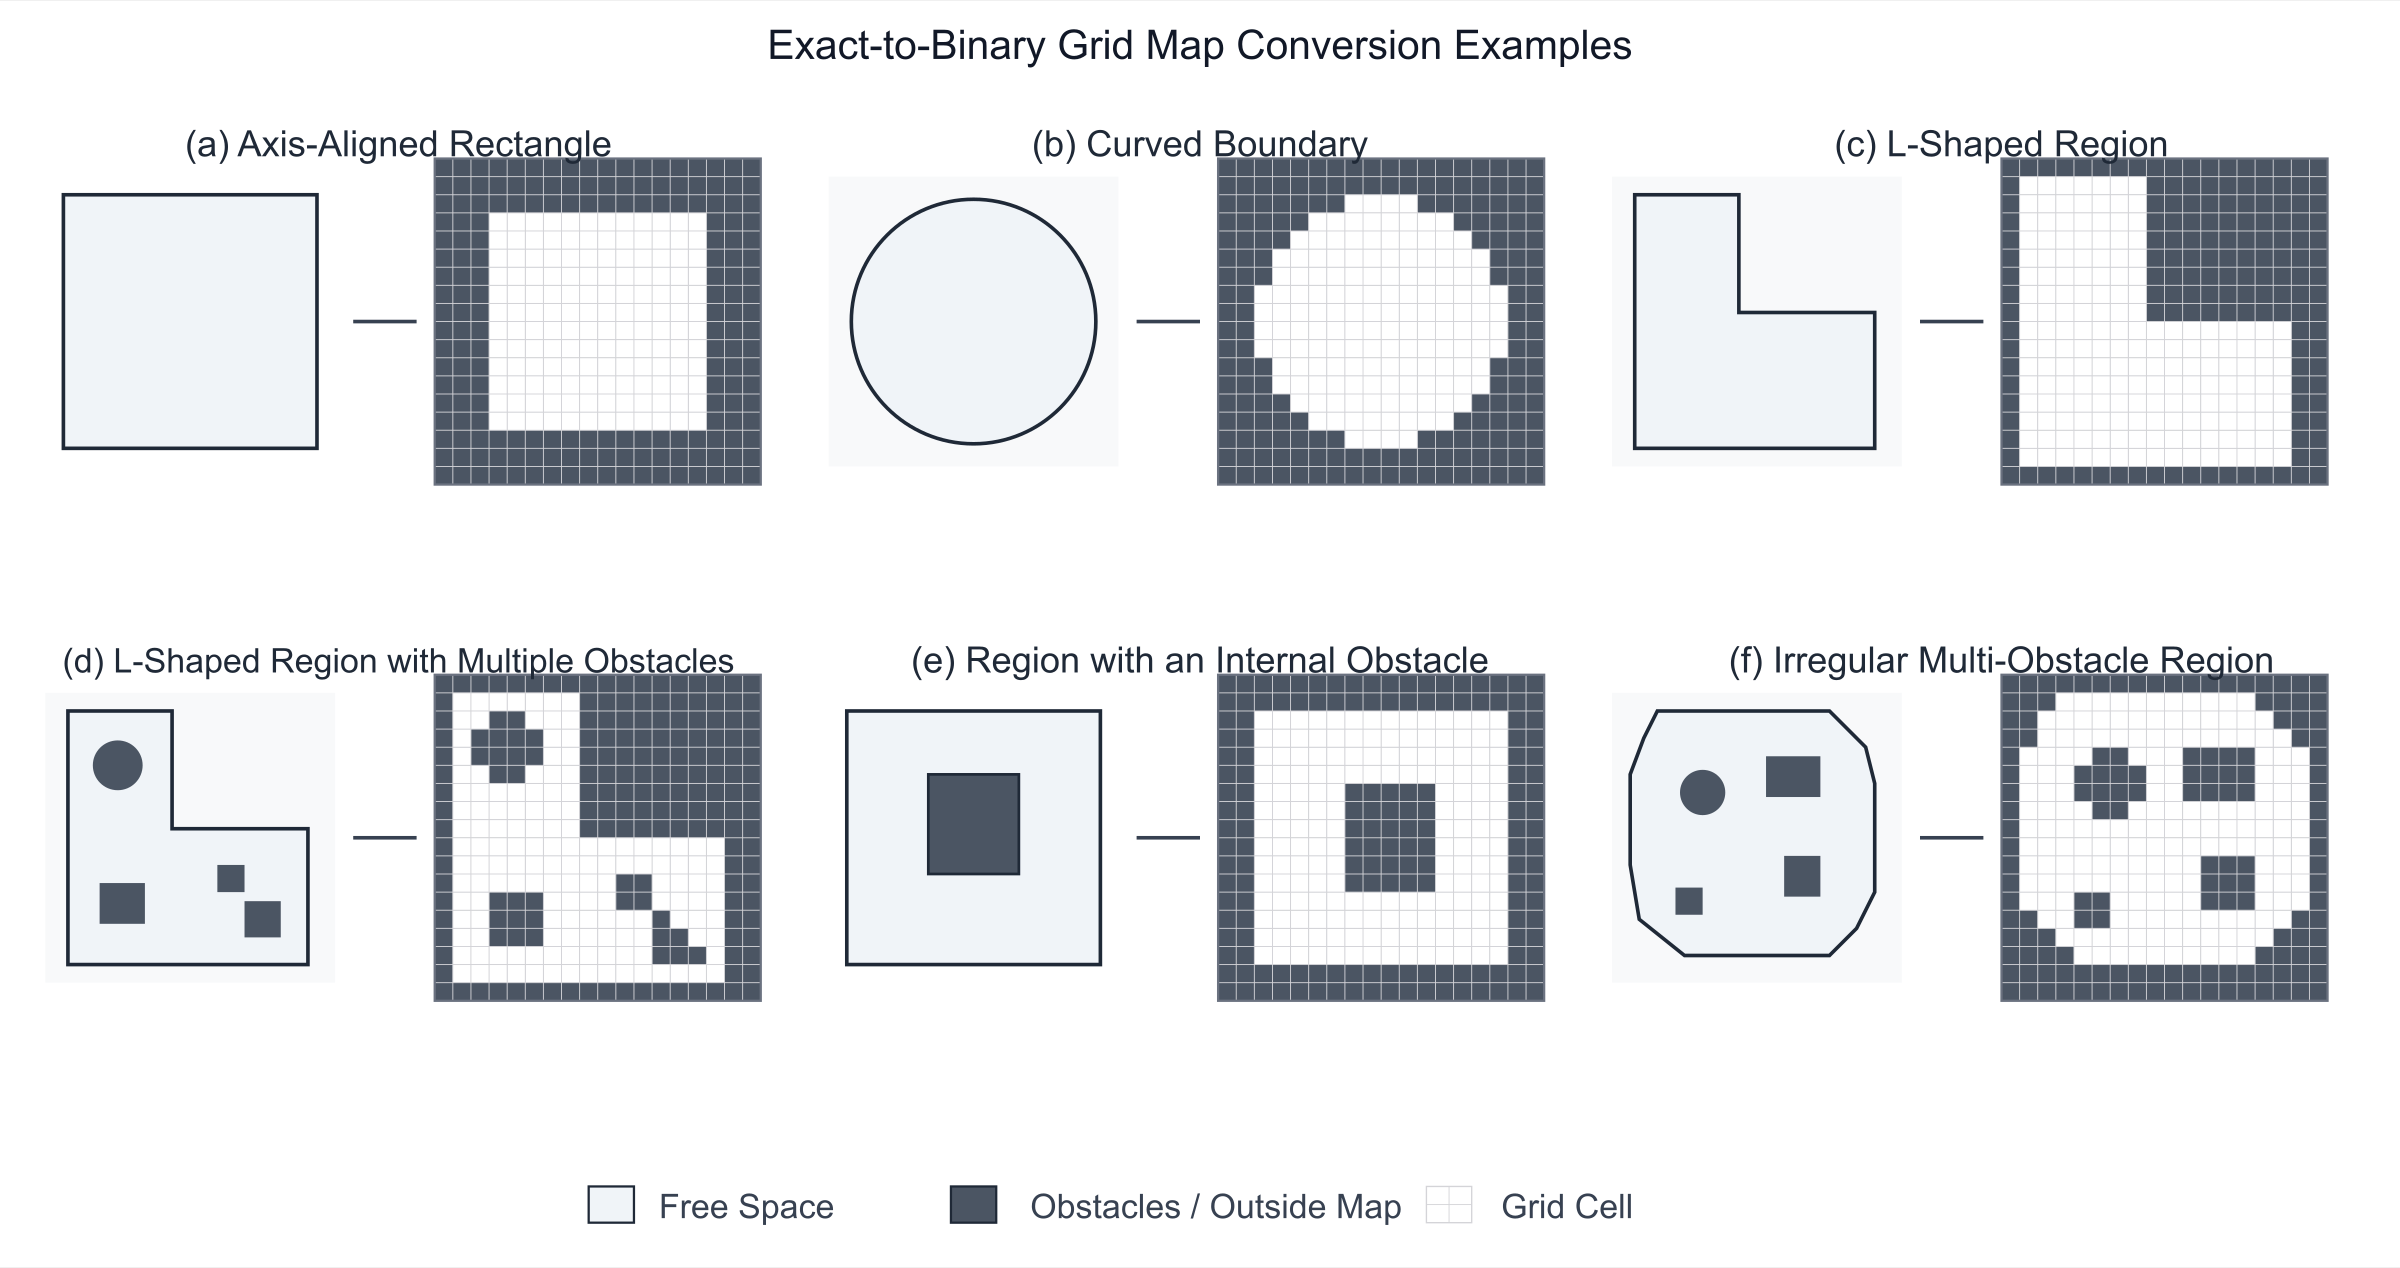
\includegraphics[width=\dimexpr\linewidth-2\fboxsep-2\fboxrule\relax]{old_figs/figure_3_geometric_to_binary_raster.png}}}\\[0.25em]
{\color{red}\scriptsize 修改前}
\end{minipage}\hfill
\begin{minipage}[t]{0.48\linewidth}\centering
{\setlength{\fboxsep}{1.2pt}\setlength{\fboxrule}{1.1pt}%
\fcolorbox{blue}{white}{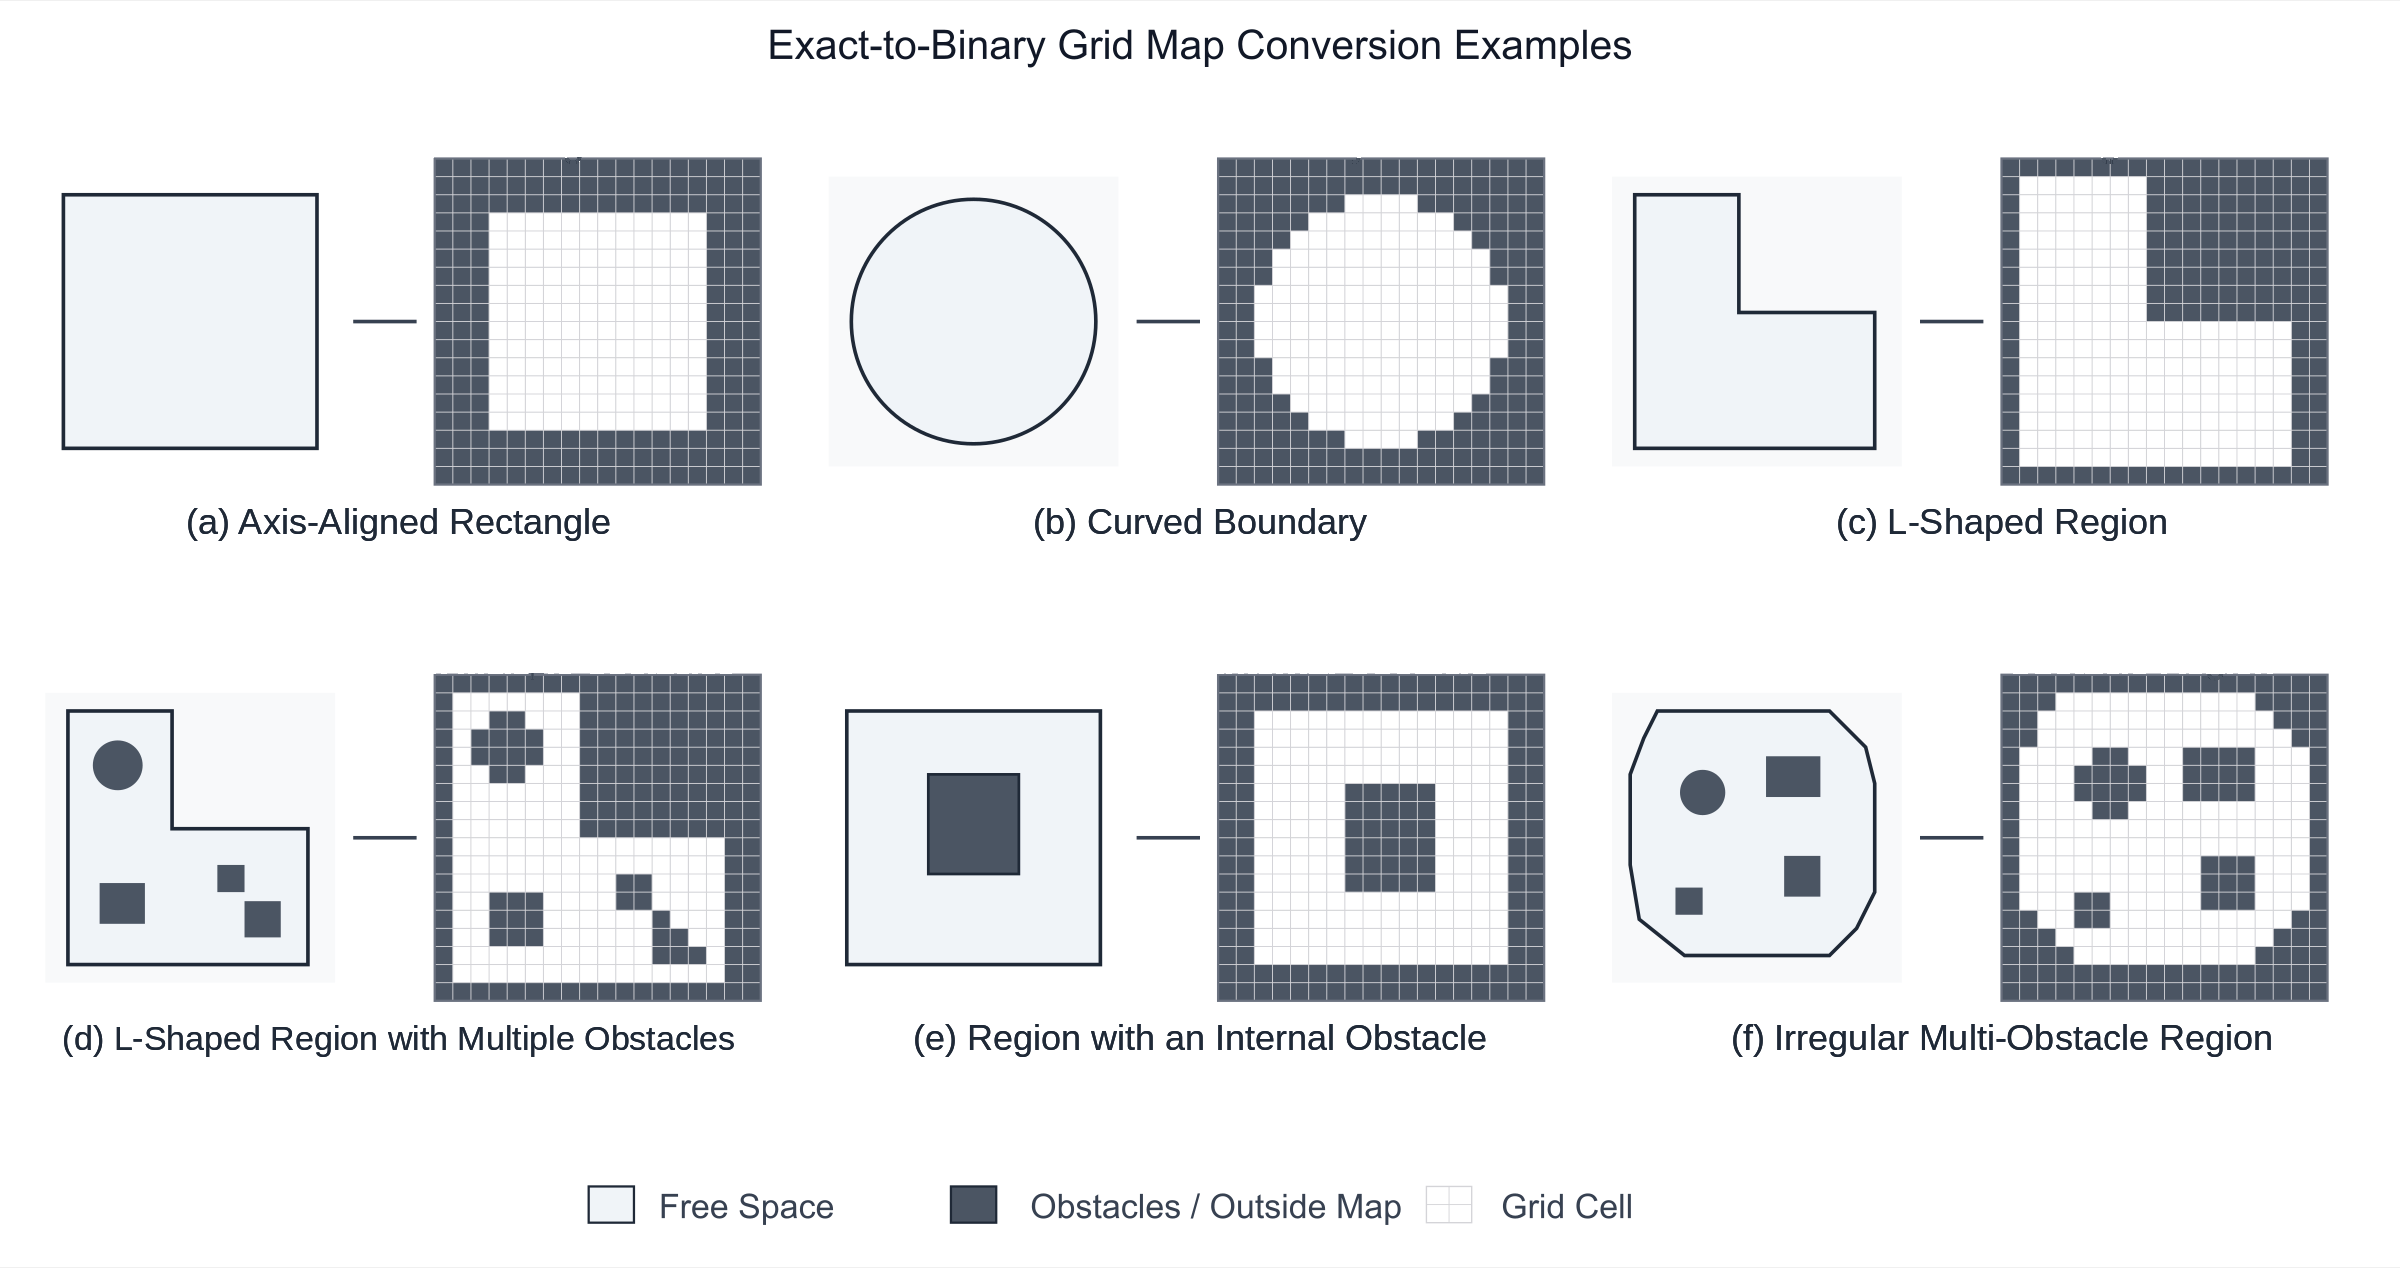
\includegraphics[width=\dimexpr\linewidth-2\fboxsep-2\fboxrule\relax]{figures/figure_3_geometric_to_binary_raster.png}}}\\[0.25em]
{\color{blue}\scriptsize 修改后}
\end{minipage}\par
% ===FIGPAIR END figure_3_geometric_to_binary_raster.png===
  \caption{Conversion from exact geometric descriptions to the binary raster input.\DIFdelbeginFL \DIFdelFL{The left column shows exact two-dimensional work regions and rectangular subregions abstracted from CAD/BIM, survey, or mapping data; the right column shows the binary map \mbox{$M$} used by the planner. White denotes free target area, black denotes obstacles, openings, or out-of-bound regions, and dashed rectangles indicate approximate cells that may support later rectangular candidates. Examples include rectangular rooms, circular or curved boundaries, L-shaped areas, T-junction or corridor connections, regions with columns or openings, and irregular areas with dense obstacles.}\DIFdelendFL }
  \label{fig:rasterization-examples}
\end{figure}\marginpar{\scriptsize [48] 把 Figure 4 各子图标题移到子图下方，总图注仍在整图下。}\marginpar{\scriptsize [49] 右下角黑格与左侧 L 形及臂上两个矩形的保守栅格不符，已按内角对齐的网格重画，并用 1-4 标出圆盘、竖干方块、臂上矩形和臂下矩形。}\marginpar{\scriptsize [50] 删去 Figure 4 图注中从左栏说明起的整段。}

After the map has been abstracted, equipment drawings, calibration tests, and controller limits provide the robot model and initial state. The scene input for one planning task is divided into map and robot components:
\begin{equation*}
\mathcal I=\left\langle\mathcal I_{\mathrm{map}},\mathcal I_{\mathrm{robot}}\right\rangle,
\end{equation*}
where
\begin{equation*}
\mathcal I_{\mathrm{map}}=\left\langle M,s_p,T_{WM}\right\rangle.
\end{equation*}
Here $M$ is the $H_p\times W_p$ binary work map generated from CAD/BIM, survey, or mapping data; $s_p$ converts pixel distance and area to metres and square metres; and $T_{WM}$ is the planar rigid transform from the map frame to the world frame, used to convert planned map coordinates into executable site coordinates.

The robot component is
\begin{equation*}
\mathcal I_{\mathrm{robot}}=\left\langle q_0,\Theta_R\right\rangle.
\end{equation*}
The initial base position, heading, and arm angle in $q_0$ are obtained from the site-localization system and arm encoder. The parameter set $\Theta_R$ contains the base length $l_c$ and width $w_c$, arm-link collision radius $r_a$, troweling-disc radius $r_d$ (diameter $2r_d$), arm length $L$, distance $d_p$ from the base center to the arm pivot, arm-angle limits, maximum base linear and angular velocities, and maximum arm angular velocity. Together, these parameters determine occupied geometry, the disc coverage footprint, and trajectory executability.

\begin{figure}[htbp]
  \centering
  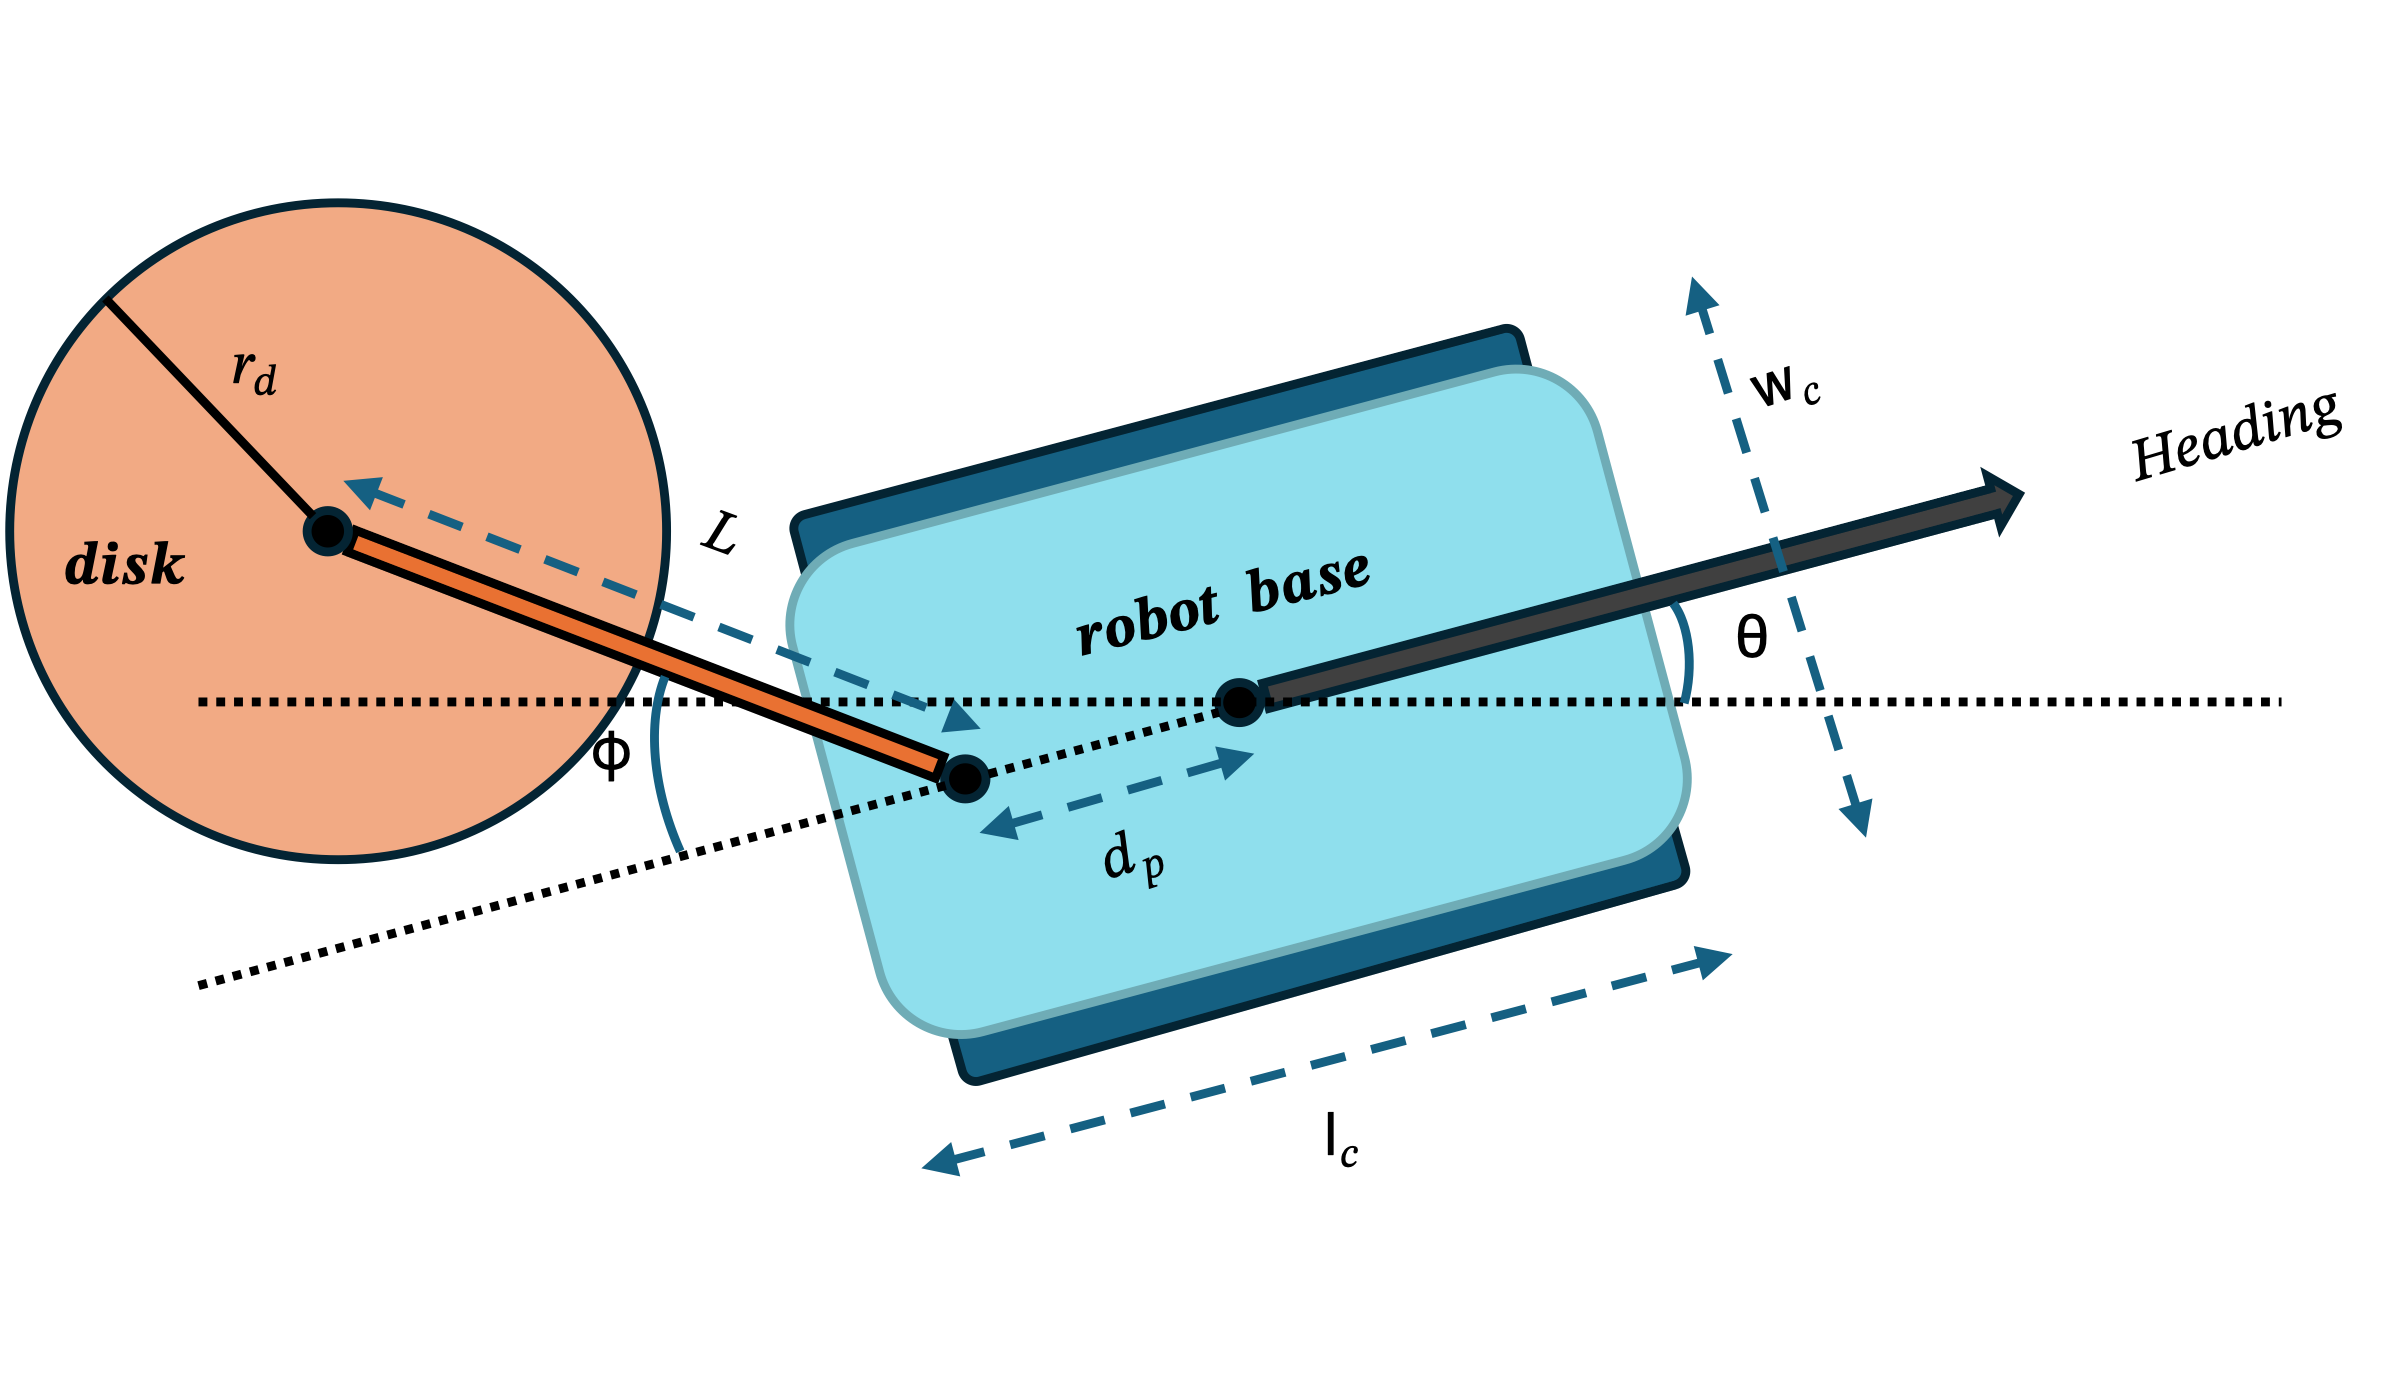
\includegraphics[width=0.82\linewidth]{figure_4_body_arm_disc_model.png}
  \caption{Geometry and motion parameters of the base--arm--disc system.\DIFdelbeginFL \DIFdelFL{The diagram identifies the base center, heading \mbox{$\theta$}, relative arm angle \mbox{$\phi$}, disc radius \mbox{$r_d$}, arm length \mbox{$L$}, base-center-to-pivot offset \mbox{$d_p$}, and base length and width \mbox{$l_c,w_c$}. These quantities determine the robot's occupied geometry and the disc-center position in Eq.~\mbox{\eqref{eq:disc-center}}.}\DIFdelendFL }
  \label{fig:robot-geometry}
\end{figure}\marginpar{\scriptsize [52] 删去 Figure 5 图注中罗列符号的句子。}

In addition to these scene inputs, the algorithm uses a planning configuration $\Psi_P$: planning-cell size $g$, minimum rectangle side length, candidate-selection parameters $\alpha$ and $\beta$, candidate truncation count, scan and connectivity strategies, and random seed. The configuration controls decomposition and search but is not part of the map or robot model abstracted from the physical scene.

\subsubsection{Planning Model and Notation}

Let the input map be
\begin{equation*}
M\in\{0,255\}^{H_p\times W_p},
\end{equation*}
\DIFdelbegin \DIFdel{where \mbox{$M_{uv}=0$} is an obstacle pixel and \mbox{$M_{uv}=255$} a free pixel}\DIFdelend \DIFaddbegin \DIFadd{The labels $0$ and $255$ are 8-bit pixel labels, not physical sizes or continuous geometric quantities}\marginpar{\scriptsize [51] 说明 0 和 255 只是障碍与自由的标签，未改图像编码。}\marginpar{\scriptsize 将 0 和 255 改写为 8-bit 像素标签，不是物理尺寸或连续的几何量。}\DIFaddend . With physical pixel size $s_p$, the free-pixel set is
\begin{equation*}
\mathcal P_F=\{(u,v)\mid M_{uv}=255\}.
\end{equation*}
All subsequent positions and distances are transformed by $T_{WM}$ into a metric world frame; for clarity, the transform is omitted from the remaining notation.

The robot state is
\begin{equation*}
q(t)=\bigl(x_c(t),y_c(t),\theta(t),\phi(t)\bigr),
\end{equation*}
with state space $\mathcal Q=\mathbb R^2\times S^1\times[\phi_{\min},\phi_{\max}]$. Here $(x_c,y_c)$ is the base center, $\theta$ the base heading, and $\phi$ the arm angle relative to the base. Let $\mathbf p_c=(x_c,y_c)$ and $\mathbf e(\gamma)=(\cos\gamma,\sin\gamma)$. For arm length $L$ and base-center-to-pivot offset $d_p$, the center of the circular disc is
\begin{equation}
\mathbf p_d(q)=\mathbf p_c-d_p\mathbf e(\theta)+L\mathbf e(\theta+\pi+\phi).
\tag{1}
\label{eq:disc-center}
\end{equation}
Equation~\eqref{eq:disc-center} is the sum of two translations: from the base center to the arm pivot and from the pivot to the disc center. As shown in Fig.~\ref{fig:robot-geometry}, $\mathbf e(\theta)$ points along the base heading, and the pivot lies $d_p$ behind the base center, so
\begin{equation*}
\mathbf p_p=\mathbf p_c-d_p\mathbf e(\theta).
\end{equation*}
The arm angle $\phi$ is defined as the signed rotation from the rearward base axis, positive counterclockwise. Since the rearward axis is rotated by $\pi$ from the forward heading, the pivot-to-disc direction is $\theta+\pi+\phi$, and its displacement is $L\mathbf e(\theta+\pi+\phi)$. For example, when $\theta=0$ and $\phi=0$, the base faces the positive world $x$-axis, the pivot is at $(x_c-d_p,y_c)$, and the disc center is at $(x_c-d_p-L,y_c)$: the arm extends directly behind the base. Changing $\theta$ rotates the pivot and arm with the base; changing $\phi$ at fixed $\theta$ moves the disc center along a radius-$L$ arc about the pivot.

For disc radius $r_d$, the instantaneous work region at one pose is
\begin{equation}
\mathcal D(q)=\{\mathbf z\in\mathbb R^2\mid\|\mathbf z-\mathbf p_d(q)\|_2\le r_d\}.
\tag{2}
\label{eq:instantaneous-disc}
\end{equation}
The region swept by a continuous trajectory $q:[0,T]\rightarrow\mathcal Q$ is
\begin{equation}
\mathcal C(q)=\bigcup_{t\in[0,T]}\mathcal D(q(t)).
\tag{3}
\label{eq:swept-area}
\end{equation}

To distinguish disc reachability from whole-robot feasibility, let $\mathcal O_M$ be the unavailable region corresponding to black pixels in world coordinates, $\mathcal B(q)$ the rotated $l_c\times w_c$ base rectangle, and $\mathcal A(q)$ a capsule of radius $r_a$ around the arm link. A state is geometrically feasible only if
\begin{equation}
\bigl(\mathcal B(q)\cup\mathcal A(q)\cup\mathcal D(q)\bigr)\cap\mathcal O_M=\varnothing.
\tag{3a}
\label{eq:geometric-feasibility}
\end{equation}
All feasible states form $\mathcal Q_F\subseteq\mathcal Q$. For a motion segment $q_s:[0,T_s]\rightarrow\mathcal Q$, the method requires $q_s(t)\in\mathcal Q_F$ for every $t\in[0,T_s]$ and
\begin{equation}
|v(t)|\le v_{\max},\qquad
|\dot\theta(t)|\le\omega_{\max},\qquad
|\dot\phi(t)|\le\omega_{a,\max}.
\tag{3b}
\label{eq:velocity-limits}
\end{equation}
Straight motion, in-place rotation, arm adjustment, and other primitives are adaptively subdivided, and Eq.~\eqref{eq:geometric-feasibility} is checked over every subinterval. Consequently, later rectangle adjacencies and entry states are candidates only; a transfer enters the final planning graph only after passing this check.

Under Eqs.~\eqref{eq:geometric-feasibility} and \eqref{eq:velocity-limits}, the algorithm is assessed at three levels: \DIFdelbegin \DIFdel{work quality}\DIFdelend \DIFaddbegin \DIFadd{effective-work coverage}\marginpar{\scriptsize [53] 将目标中的 work quality 改为 effective-work coverage，引言中改为 surface finish。}\DIFaddend , trajectory-execution efficiency, and planning efficiency. The corresponding objectives are
\begin{equation}
\max \rho_{\mathrm{work}}(q),\qquad
\min T_{\mathrm{exec}}(q),\qquad
\min T_{\mathrm{plan}}.
\tag{4}
\label{eq:objectives}
\end{equation}
The effective-work coverage ratio $\rho_{\mathrm{work}}(q)$ is the fraction of the target area swept by the disc during work-labeled segments. The nominal execution time $T_{\mathrm{exec}}(q)$ runs from the initial state to completion and includes the initial connection, effective work, turns, arm adjustments, and inter-region transfers. The wall-clock planning time $T_{\mathrm{plan}}$ covers the algorithm from conservative-grid generation through trajectory assembly and coverage evaluation.

These measures play distinct roles. The task-level\marginpar{\scriptsize [54] 将 task-level quality measure 改为 task-level coverage measure。} \DIFdelbegin \DIFdel{quality }\DIFdelend \DIFaddbegin \DIFadd{coverage }\DIFaddend measure $\rho_{\mathrm{work}}$ is encouraged indirectly through free-space rectangle representation, rewards for new coverage, and overlap penalties, then computed from the continuous disc sweep in Eqs.~\eqref{eq:disc-center}--\eqref{eq:swept-area} after the complete trajectory is available. The \DIFdelbegin \DIFdel{route-level objective }\DIFdelend \DIFaddbegin \DIFadd{search uses time proxies of local coverage, transit, and transfer to compare visitation sequences; the full execution time }\DIFaddend $T_{\mathrm{exec}}$ \DIFdelbegin \DIFdel{supplies time costs to local primitives and global visitation candidates; the }\DIFdelend \DIFaddbegin \DIFadd{is computed after the trajectory has been generated and is not used as a cost in the search. The }\marginpar{\scriptsize [55] 把搜索代价改为局部时间代理，全程时间不进入搜索。}\DIFaddend algorithm selects feasible trajectories with low proxy cost but does not claim a global minimum. The planning-time measure $T_{\mathrm{plan}}$ is not a decision variable of $q$; it is a design objective controlled by hierarchical decomposition, polynomial-time heuristics, and candidate truncation. This separation motivates the hierarchical heuristic framework.

\subsection{Conservative Rasterization and Rectangular Decomposition}

\DIFdelbegin \DIFdel{The decomposition module first converts the pixel map into a coarser planning grid}\DIFdelend \DIFaddbegin \DIFadd{Following the conservative rule of Section~\ref{sec:scene-inputs}, the test is written here on planning cells}\marginpar{\scriptsize [56] 用一句沿用前文保守规则并接上公式，不再重讲栅格化。}\DIFaddend . Let each square planning cell contain $g\times g$ pixels, and let $\Omega_{ij}$ be the pixel block associated with planning cell $(i,j)$\DIFdelbegin \DIFdel{. Conservative rasterization gives
}\DIFdelend \DIFaddbegin \DIFadd{:
}\DIFaddend \begin{equation}
B_{ij}=\begin{cases}
1, & \text{if } M_{uv}=255,\quad \forall (u,v)\in\Omega_{ij},\\
0, & \text{otherwise}.
\end{cases}
\tag{5}
\label{eq:conservative-raster}
\end{equation}
\DIFdelbegin \DIFdel{Thus, \mbox{$B_{ij}=1$} means that the planning cell can support rectangle generation; \mbox{$B_{ij}=0$} means that it contains or touches an obstacle. The rule sacrifices some free area near obstacles but guarantees that subsequent rectangular candidates do not cross known obstacles.
}%DIFDELCMD < 

%DIFDELCMD < %%%
\DIFdelend On $B$, the algorithm scans maximal contiguous runs of free cells by rows and by columns, extending them across adjacent scan lines as long as every enclosed cell remains free. This produces axis-aligned candidates of the form
\begin{equation}
R=[x_1,x_2]\times[y_1,y_2],
\tag{6}
\label{eq:rectangle}
\end{equation}
\DIFdelbegin \DIFdel{with all }\DIFdelend \DIFaddbegin \DIFadd{All }\DIFaddend planning cells inside\marginpar{\scriptsize [57] 在矩形定义后另写一句话说明矩形内规划格均为自由。} $R$ \DIFaddbegin \DIFadd{are }\DIFaddend free. Candidates whose width or height is below a specified minimum are removed. The remainder are ordered first by decreasing area and, for equal areas, by increasing row and column coordinates of the upper-left and then lower-right corner. Only the first $C_{\max}$ candidates from each scan direction are retained. This deterministic truncation controls rapid growth in candidate count while making the candidate set repeatable for fixed inputs and parameters.

Candidate selection is formulated as a penalized maximum-coverage problem. Let $\mathcal U(R)$ be the set of planning cells covered by $R$ and $\mathcal A$ the cells already covered by selected rectangles. The marginal utility of selecting $R$ is
\begin{equation}
\Delta(R\mid\mathcal A)=|\mathcal U(R)\setminus\mathcal A|-\alpha-\beta|\mathcal U(R)\cap\mathcal A|.
\tag{7}
\label{eq:marginal-utility}
\end{equation}
\DIFdelbegin \DIFdel{Cardinalities are measured in }\marginpar{\scriptsize [58] 删去 Cardinalities，并说明绝对值是规划格个数，公式未改。}\DIFdelend \DIFaddbegin \DIFadd{The absolute values in Eq.~\eqref{eq:marginal-utility} are counts of }\DIFaddend planning cells, so $\alpha$ has units of cells and $\beta$ is dimensionless. The first term rewards new coverage; the other terms penalize rectangle count and overlap. The algorithm repeatedly selects the row-scan candidate with the largest positive marginal utility, using the deterministic ordering above to break ties. It then processes the column-scan pool relative to the current $\mathcal A$, so column-oriented rectangles mainly supplement vertical structures poorly represented by row scans. The two greedy stages produce the initial selection.

Candidate truncation or the penalties may leave a small number of free cells uncovered. A deterministic hole-filling stage therefore selects the first uncovered free cell in row-major order as a seed, enumerates maximal axis-aligned obstacle-free rectangles containing the seed, and selects the largest. Remaining ties are resolved by rectangle width and upper-left coordinates. The selected rectangle is added and $\mathcal A$ updated until every usable planning cell belongs to at least one rectangle. The resulting set, before connectivity repair, is $\mathcal R_1$. Minimum side length, $C_{\max}$, $\alpha$, $\beta$, and scan direction are included in $\Psi_P$.

\subsection{\DIFdelbegin \DIFdel{Connectivity Completion and Final Segmentation}\DIFdelend \DIFaddbegin \DIFadd{Connectivity Completion}\DIFaddend }\marginpar{\scriptsize [59] 将小节标题改为连通补全，不再使用 final segmentation。}

Covering every free planning cell with rectangles does not ensure that the robot can move continuously between them. The method therefore constructs an undirected graph
\begin{equation}
G=(V,E),
\tag{8}
\label{eq:feasible-graph}
\end{equation}
over $\mathcal R_1$, with node $v_i\in V$ representing rectangle $R_i$. Shared boundaries, contact, and overlap generate geometric adjacency candidates only. For each candidate pair $(R_i,R_j)$, a finite set of handoff poses is generated in the intersection or along the closest opposing boundaries. The algorithm then attempts to connect an exit state of the first rectangle to an entry state of the second. Edge $(v_i,v_j)$ is added only if at least one transfer primitive satisfies Eqs.~\eqref{eq:geometric-feasibility} and \eqref{eq:velocity-limits}. The edge stores the minimum time proxy $c_{ij}$ among all feasible handoffs. Graph $G$ consequently represents executable robot transfers, not merely geometric contact between rectangles.

If $G$ has multiple connected components, the algorithm searches the unselected candidates for bridging rectangles. A candidate $R_b$ is a bridge if, after insertion, it forms feasible edges with rectangles in at least two previously distinct components. Preference is given to rectangles with little new area and low feasible-transfer cost:
\begin{equation}
R_b^\star=\arg\min_{R_b\in\mathcal B}\left(|\mathcal U(R_b)\setminus\mathcal A|+\lambda_b\sum c_{ib}\right),
\tag{9}
\label{eq:bridge-cost}
\end{equation}
where $\mathcal B$ is the current bridge-candidate set, the sum contains only edges used to connect components, and $\lambda_b$ weights transfer time. Relevant edges and connected components are recomputed after every insertion, until $G$ becomes connected. \DIFaddbegin \DIFadd{The final rectangle set $\mathcal R$ is $\mathcal R_1$ after the bridging rectangles have been added. }\DIFaddend If $\mathcal B$ is empty while $G$ remains disconnected, no single continuous coverage trajectory is supported by the current candidate set and parameters. The method reports connectivity failure and does not proceed to global route planning.

\DIFdelbegin %DIFDELCMD < \begin{algorithm}[htbp]
%DIFDELCMD < %%%
\DIFdelend \DIFaddbegin \begin{algorithm}[H]
\DIFaddend \caption{Rectangle segmentation and connectivity completion}
\label{alg:segmentation}
\small
\begin{algorithmic}[1]
\Require Conservative free-cell grid $B$, planning parameters $\Psi_P$, robot model $\Theta_R$
\Ensure Rectangle set $\mathcal R$ and feasible graph $G$, or connectivity failure
\State $F\gets\{u:B(u)=1\}$; $\mathcal R\gets\varnothing$; $\mathcal A\gets\varnothing$
\State $(C_r,C_c)\gets\mathrm{ScanAndTruncate}(B,\Psi_P)$
\State $C_{\mathrm{all}}\gets C_r\cup C_c$
\For{$C\in(C_r,C_c)$, in this order}
  \While{$\exists R\in C:\Delta(R\mid\mathcal A)>0$}
    \State $R^\star\gets\arg\max_{R\in C}\Delta(R\mid\mathcal A)$ \Comment{Eq.~\eqref{eq:marginal-utility}; deterministic ties}
    \State $\mathcal R\gets\mathcal R\cup\{R^\star\}$; $\mathcal A\gets\mathcal A\cup\mathcal U(R^\star)$
    \State $C\gets C\setminus\{R^\star\}$
  \EndWhile
\EndFor
\While{$\mathcal A\neq F$}
  \State $u\gets\mathrm{FirstUncovered}(F\setminus\mathcal A)$
  \State $R^\star\gets\mathrm{LargestMaximalRectangle}(B,u)$ \Comment{deterministic ties}
  \State $\mathcal R\gets\mathcal R\cup\{R^\star\}$; $\mathcal A\gets\mathcal A\cup\mathcal U(R^\star)$
\EndWhile
\State $\mathcal R_1\gets\mathcal R$; $G\gets\mathrm{FeasibleGraph}(\mathcal R_1,\Theta_R)$
\While{$G$ is disconnected}
  \State $\mathcal B\gets\mathrm{FeasibleBridges}(C_{\mathrm{all}}\setminus\mathcal R,G,\Theta_R)$
  \If{$\mathcal B=\varnothing$}
    \State \Return connectivity failure
  \EndIf
  \State $R_b^\star\gets\mathrm{MinBridgeCost}(\mathcal B)$ \Comment{Eq.~\eqref{eq:bridge-cost}}
  \State $\mathcal R\gets\mathcal R\cup\{R_b^\star\}$; $G\gets\mathrm{UpdateFeasibleGraph}(G,R_b^\star)$
\EndWhile
\State \Return $(\mathcal R,G)$
\end{algorithmic}
\end{algorithm}\marginpar{\scriptsize [62] 将 Algorithm 1 改为与所在小节放在一起，不跨小节浮动。}

Algorithm~\ref{alg:segmentation} summarizes the complete process from conservative rasterization to the final graph. The overlap penalty in Eq.~\eqref{eq:marginal-utility} suppresses redundant rectangles within a candidate pool; hole filling represents every free planning cell; and bridging adds rectangles only when the current set cannot form a connected feasible graph. ``Connected'' always refers to graph connectivity after complete robot-transfer checks, not merely topological connectivity of free cells or the geometric rectangle union.

Let the planning grid be $H\times W$, the truncated candidate count $C$, the final rectangle count $n$, and the mean candidate area $A$ cells. Candidate generation has worst-case complexity $O(HW(H+W))$. With a naive set implementation, greedy selection is approximately $O(CnA)$. Adjacency-candidate enumeration is $O(n^2)$, with a finite number of local-motion checks per edge. The minimum side length, candidate truncation, and deterministic ordering jointly limit practical problem size. Since later graph search and local-primitive instantiation grow with $n$, controlling the rectangle count during decomposition directly affects $T_{\mathrm{plan}}$.

\subsection{Single-Rectangle Coverage Primitive}

The rectangle-coverage module supplies the local motion primitive. Given a rectangle $R$, feasible entry pose $q^{\mathrm{in}}$, feasible exit pose $q^{\mathrm{out}}$, and robot parameters, it generates a continuous motion segment. On the first occurrence of $R$ in the global sequence, the robot executes the back-and-forth coverage shown in Fig.~\ref{fig:rectangle-primitive}; if $R$ has already been covered, only an entry-to-exit transit motion is generated. Both primitive types retain the complete robot state, duration, and work-state label.

\begin{figure}[htbp]
  \centering
  \DIFdelbeginFL %DIFDELCMD < 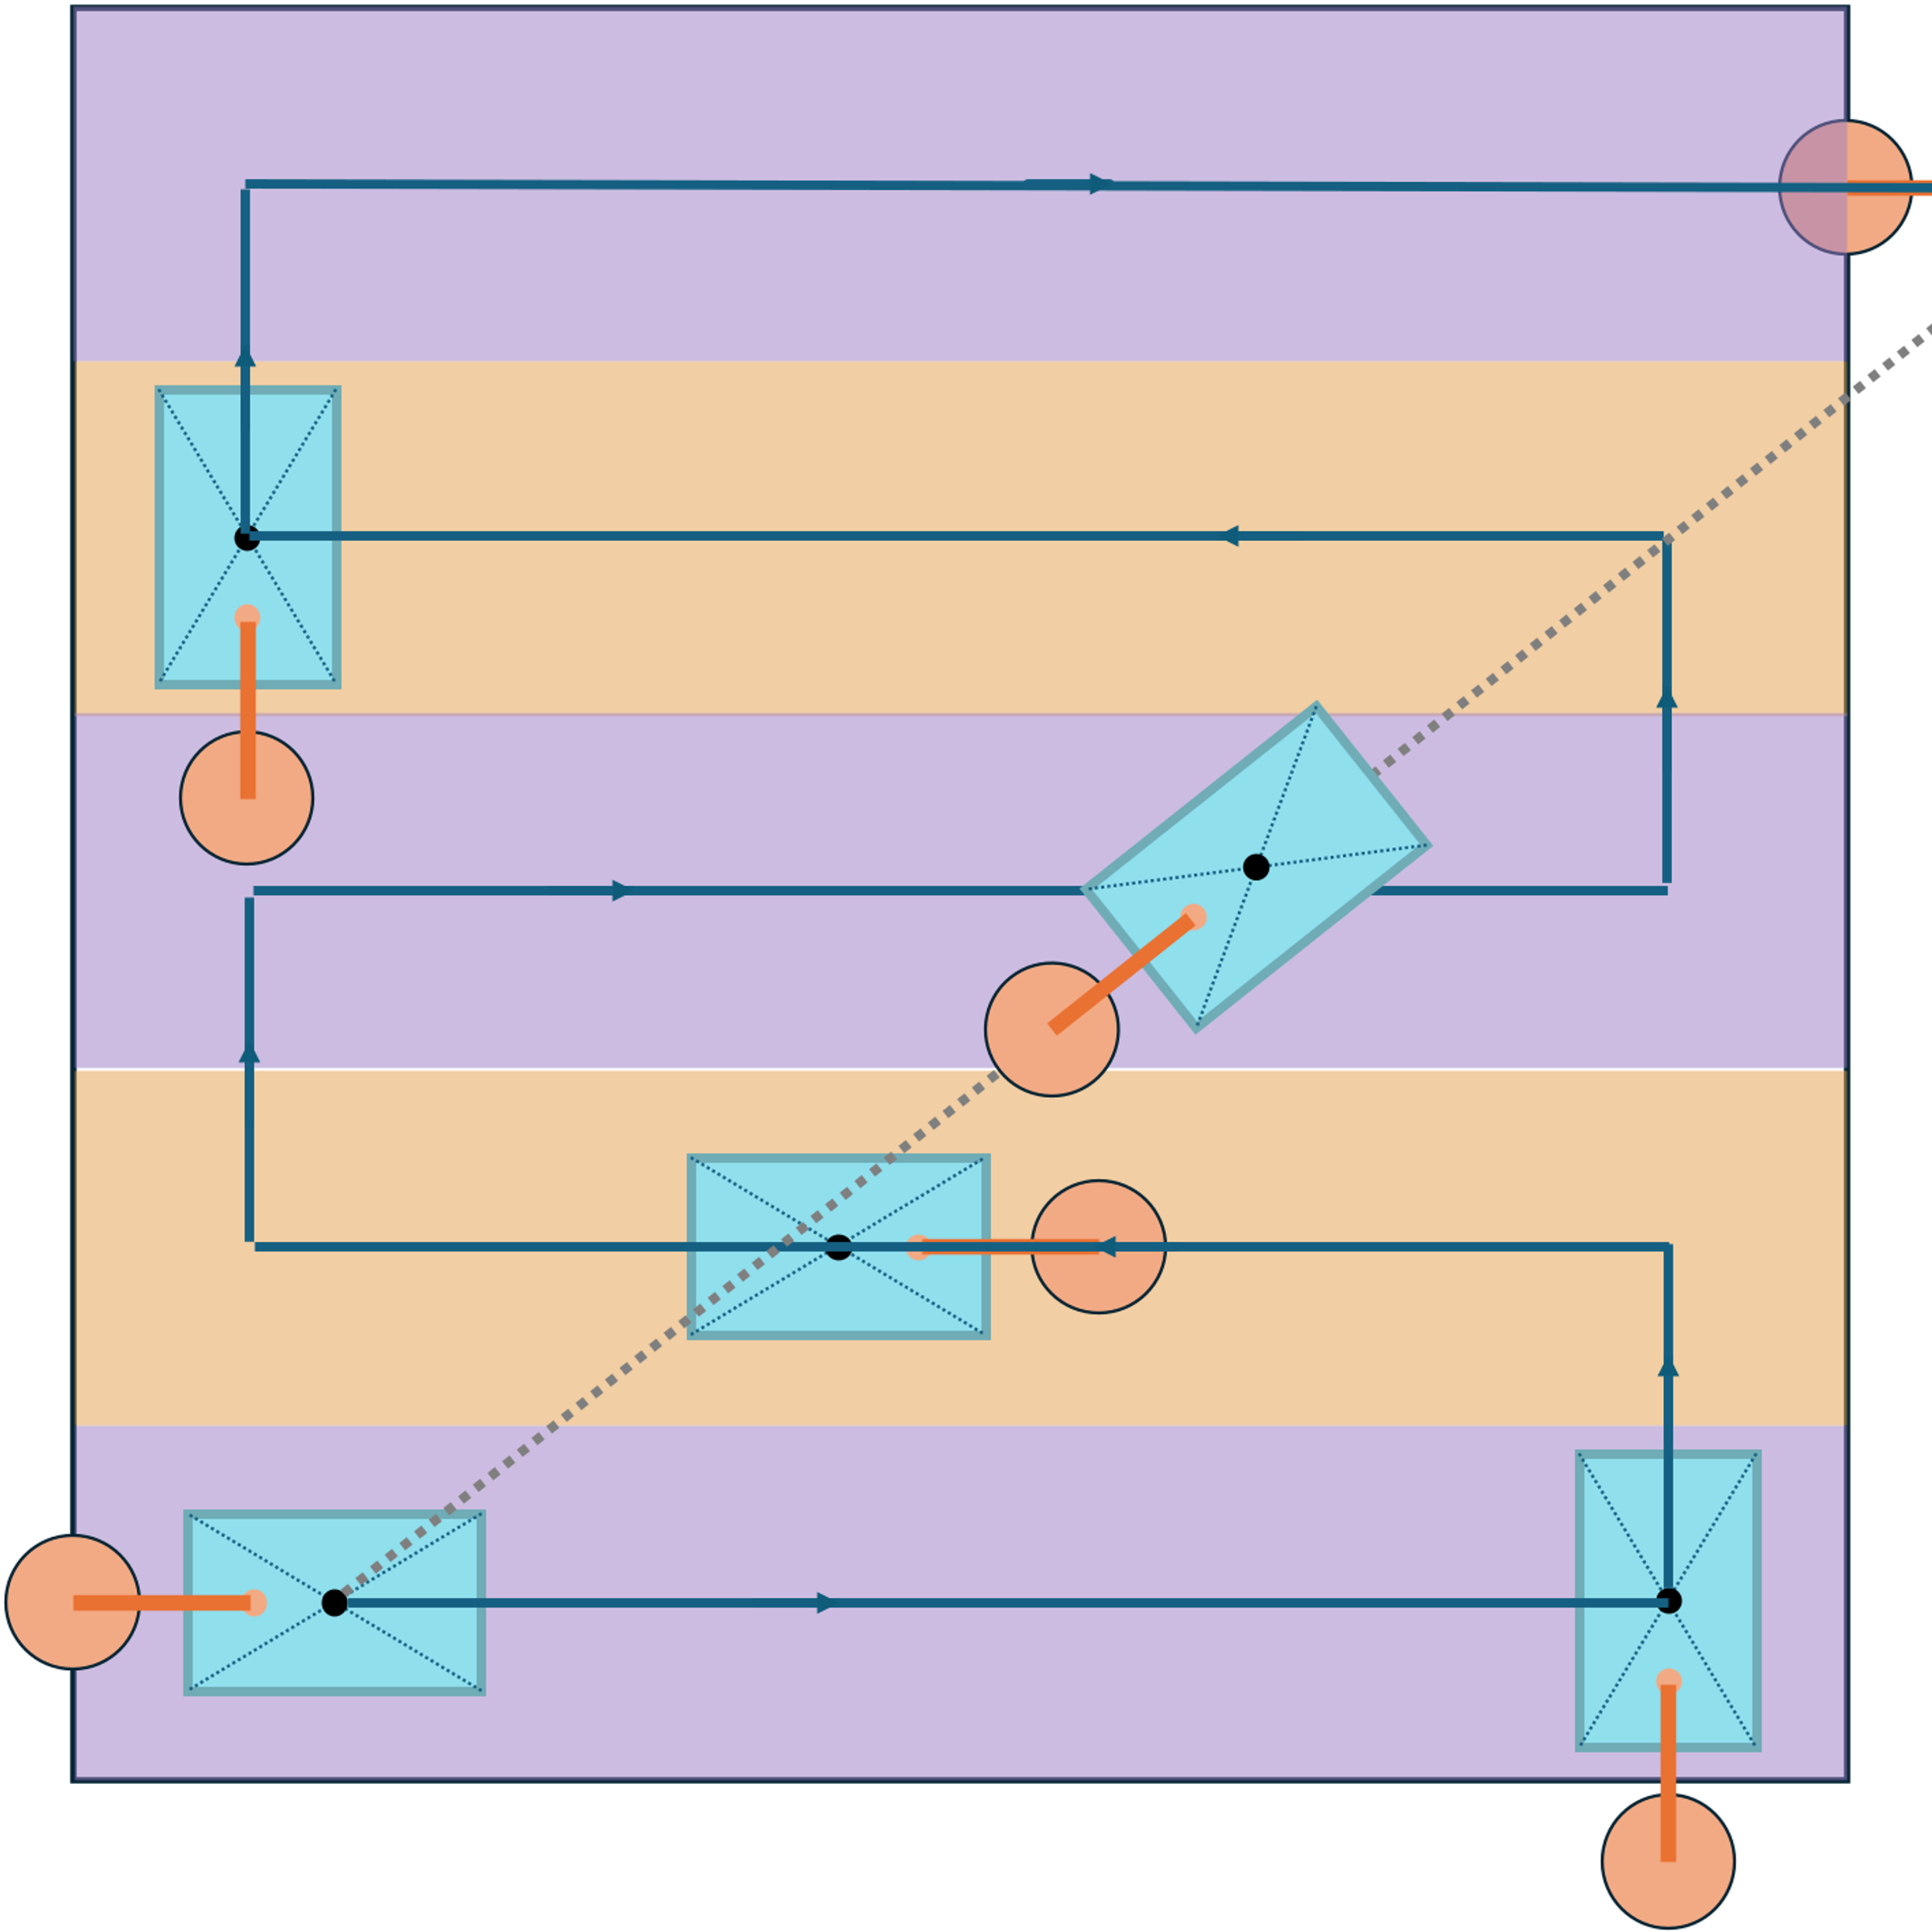
\includegraphics[width=0.84\linewidth]{figure_6_single_rectangle_coverage.png}
%DIFDELCMD <   %%%
\DIFdelendFL \DIFaddbeginFL 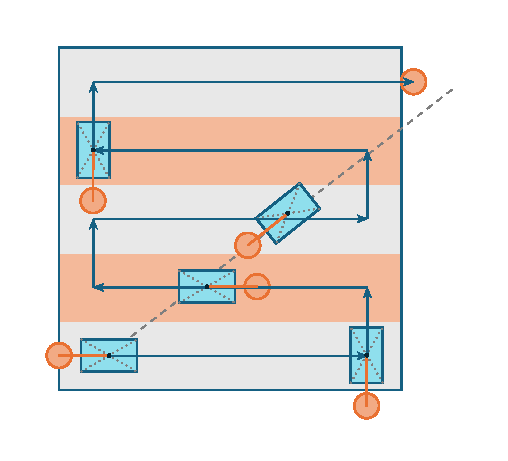
\includegraphics[width=0.5\linewidth]{figure_6_single_rectangle_coverage.pdf}
  \DIFaddendFL \caption{Single-rectangle coverage primitive.\DIFdelbeginFL \DIFdelFL{The disc entry and exit are determined by neighboring rectangles or the initial state. The local planner compares time proxies for both sweep directions and feasible starting corners, then covers the rectangle through forward base motion and reciprocal arm swinging.}\DIFdelendFL }
  \label{fig:rectangle-primitive}
\end{figure}\marginpar{\scriptsize [61] 删去 Figure 6 图注的后半句。}

\DIFaddbegin \DIFadd{Local paths are not redrawn for other aspect ratios. Each local path is a back-and-forth strip along one axis of the rectangle: the longer side is the default so as to reduce lane changes, and the other axis is also generated and compared by time.
}\marginpar{\scriptsize [60] 把 Figure 6 缩到约半栏宽，并说明不按长宽比另画路径。}

\DIFaddend \subsubsection{Entry and Exit Poses}

Entry and exit candidates are jointly determined by the predecessor and successor of a rectangle in the visitation sequence. If $R_i$ is followed by $R_j$, a finite set of disc handoff points is sampled uniformly in their shared region or along their opposing boundaries. An entry to the first rectangle must also be reachable from $q_0$, and an exit from the final rectangle is selected among its remaining feasible boundary candidates. Each candidate specifies the disc center, base heading, and reference arm angle rather than only a boundary point.

For disc points on the left, right, lower, and upper boundaries, the nominal headings are $\pi$, $0$, $3\pi/2$, and $\pi/2$, respectively, so that the base in its retracted configuration lies outside the corresponding rectangle boundary. This rule generates nominal candidates only. Near dense obstacles or narrow boundaries, the externally positioned base may still enter unavailable space and therefore cannot be accepted without checking.

Given a boundary pose $(\mathbf p_d,\theta)$ for the disc center, the base center in the retracted reference configuration is recovered as
\begin{equation}
\mathbf p_c=\mathbf p_d+(d_p+L)\mathbf e(\theta).
\tag{10}
\label{eq:entry-base-center}
\end{equation}
The state and its connection from the preceding primitive are then checked against Eqs.~\eqref{eq:geometric-feasibility} and \eqref{eq:velocity-limits}. If a check fails, the handoff point is moved along the same boundary, followed by trials on an adjacent boundary and with the alternative heading. Only candidates with a feasible complete connection enter the local cost comparison. If a visit admits no feasible entry--exit pair, the corresponding global sequence cannot be instantiated.

\subsubsection{Starting Corner, Strip Width, and Swing Amplitude}

\DIFaddbegin \DIFadd{The swing amplitude is the half-amplitude of the arm angle about its neutral position while one strip is covered. It is denoted $\phi_w$ and is determined by the strip width, the disc radius, and the arm length. A work strip is one working band covered by the disc as it travels back and forth along one side of the rectangle. }\marginpar{\scriptsize [64] 在条带小节开头定义 swing amplitude 为臂角半幅，公式未改。}\marginpar{\scriptsize [65] 在长度和宽度符号之前定义 work strip。}\DIFaddend Let $\ell_R$ and $h_R$ be the rectangle dimensions parallel and perpendicular to the work strips. \DIFaddbegin \DIFadd{$\ell_R$ is the travel length of one work strip, and $h_R$ is the transverse width crossed together by the strips. }\DIFaddend The local planner uses the longer axis by default to reduce lane changes, but also generates a solution along the other axis. Across the two sweep directions and their feasible starting corners, it compares the total time proxy for entry connection, coverage, lane changes, and exit connection. Thus $h_R$ always denotes the transverse extent crossed collectively by the strips, whereas $\ell_R$ is the travel length of one strip.

\DIFaddbegin \begin{figure}[htbp]
  \centering
  % ===FIGNEW figure_strip_geometry.png===
{\setlength{\fboxsep}{1.2pt}\setlength{\fboxrule}{1.1pt}%
\fcolorbox{blue}{white}{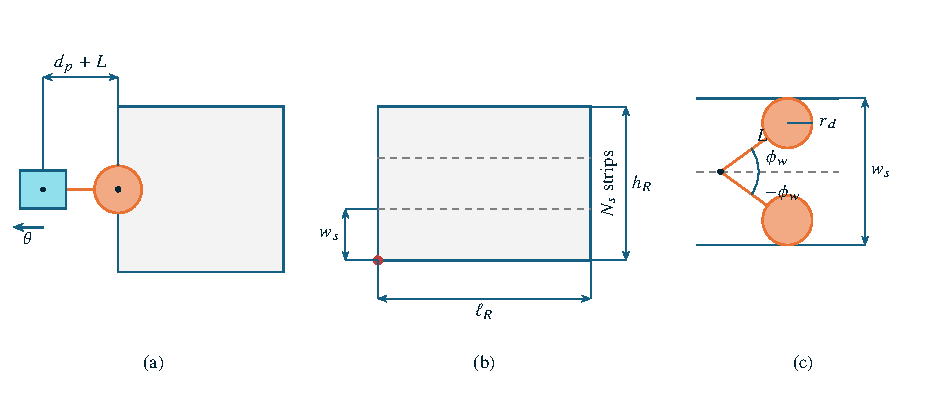
\includegraphics[width=0.92\linewidth]{figures/figure_strip_geometry.pdf}}}\\[0.25em]
{\color{blue}\scriptsize 新增}
% ===FIGNEW END figure_strip_geometry.png===
  \caption{\DIFaddFL{Entry pose, work strips, and swing amplitude $\phi_w$ for one rectangle.}}
  \label{fig:strip-geometry}
\end{figure}\marginpar{\scriptsize [63] 用已有几何符号为条带和半周期运动新画两张原理图。}\marginpar{\scriptsize 将条带数从水平顶边移到沿 h\_R 排列的条带组旁，写成 N\_s strips。顶边只保留矩形边界。}

\DIFaddend For each sweep direction, the planner filters the four corners to retain starting points reachable from the entry and connectable to the exit; the parity of the strip count determines the coverage endpoint. It selects the feasible combination with the minimum sum of non-working motion and local coverage time. Entry, sweep direction, starting corner, strip-count parity, and exit therefore jointly determine the primitive; the start is not chosen merely as the nearest corner in Euclidean distance.

Coverage inside the rectangle follows a Boustrophedon pattern, but the work width is not fixed. It is determined by the maximum usable arm angle and disc radius. For arm limits $[\phi_{\min},\phi_{\max}]$, the symmetric usable angle is
\begin{equation}
\phi_s=\min\{|\phi_{\min}|,|\phi_{\max}|,\pi/2\}.
\tag{11}
\label{eq:symmetric-angle}
\end{equation}
Over one full left--right swing, the lateral width approximately reachable by the disc-center path, including disc radius, is
\begin{equation}
w_{\max}=2(L\sin\phi_s+r_d).
\tag{12}
\label{eq:max-width}
\end{equation}
For transverse rectangle dimension $h_R$, the required number of strips and actual strip width are
\begin{equation}
N_s=\left\lceil\frac{h_R}{w_{\max}}\right\rceil,
\qquad
w_s=\frac{h_R}{N_s}.
\tag{13}
\label{eq:strip-count}
\end{equation}
The half-amplitude required to cover a strip of width $w_s$ is
\begin{equation}
\phi_w=\begin{cases}
0, & w_s\le 2r_d,\\
\arcsin\!\left(\dfrac{w_s/2-r_d}{L}\right), & w_s>2r_d,
\end{cases}
\tag{14}
\label{eq:swing-amplitude}
\end{equation}
clipped to $[0,\phi_s]$. This prevents systematic gaps between adjacent strips due to insufficient swing amplitude.

\subsubsection{Coupling Between Base and Arm Speeds}

\DIFaddbegin \begin{figure}[htbp]
  \centering
  % ===FIGNEW figure_speed_coupling.png===
{\setlength{\fboxsep}{1.2pt}\setlength{\fboxrule}{1.1pt}%
\fcolorbox{blue}{white}{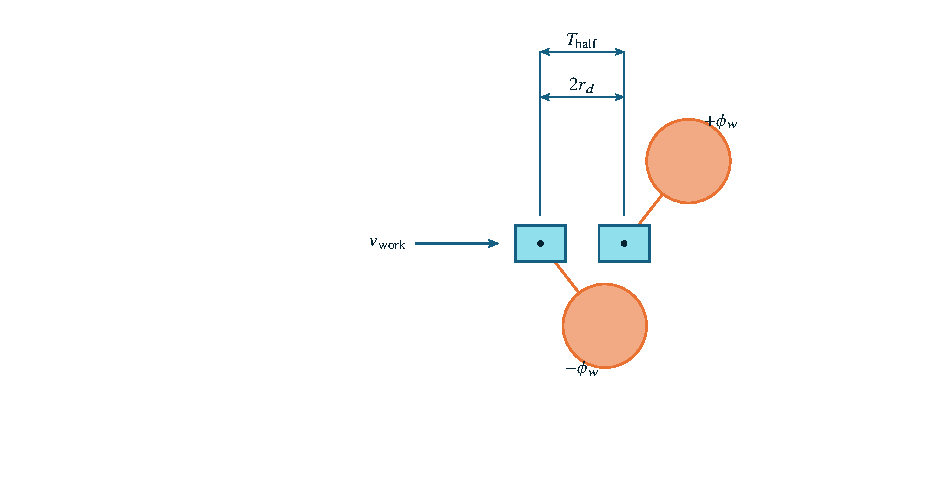
\includegraphics[width=0.78\linewidth]{figures/figure_speed_coupling.pdf}}}\\[0.25em]
{\color{blue}\scriptsize 新增}
% ===FIGNEW END figure_speed_coupling.png===
  \caption{\DIFaddFL{During one half-swing the base advances one disc diameter, so adjacent sweeps meet.}}
  \label{fig:speed-coupling}
\end{figure}

\DIFaddend Each strip combines straight base motion with periodic arm swinging. Let the maximum arm angular velocity be $\omega_{a,\max}$ and maximum base linear velocity $v_{\max}$. The time for the arm to move from $-\phi_w$ to $+\phi_w$ is
\begin{equation}
T_{\mathrm{half}}=\frac{2\phi_w}{\omega_{a,\max}}.
\tag{15}
\label{eq:half-cycle}
\end{equation}
The base work speed cannot be chosen from the mechanical limit alone if consecutive half-sweeps are to overlap sufficiently in the direction of travel. The method uses the following heuristic upper bound. If $\phi_w=0$, let $v_{\mathrm{safe}}=+\infty$; otherwise,
\begin{equation}
v_{\mathrm{safe}}=\frac{2r_d}{T_{\mathrm{half}}}.
\tag{16}
\label{eq:safe-speed}
\end{equation}
The work speed is
\begin{equation}
v_{\mathrm{work}}=\min(v_{\max},v_{\mathrm{safe}}).
\tag{17}
\label{eq:work-speed}
\end{equation}
When the arm is slow or the amplitude large, Eq.~\eqref{eq:work-speed} reduces the base speed so that the forward distance between adjacent half-sweeps does not exceed the disc diameter. This is a conservative rule derived from local sweep spacing, not a proof of complete coverage for every continuous arm trajectory. The actual swept area is therefore still checked after local motion generation by the procedure in Section~\ref{sec:coverage-evaluation}. The same \DIFdelbegin \DIFdel{relationship }\DIFdelend \DIFaddbegin \DIFadd{base--arm velocity coupling }\DIFaddend underlies the later \DIFdelbegin \DIFdel{experimental analysis of the arm-to-base speed ratio}\DIFdelend \DIFaddbegin \DIFadd{experiments}\DIFaddend .

\subsubsection{Time Model for First and Repeated Visits}

The \DIFdelbegin \DIFdel{first visit to a rectangle includes motion to the starting corner, coverage of all strips, }\DIFdelend \DIFaddbegin \DIFadd{first-visit time in Eq.~\eqref{eq:coverage-time} has four terms: strip travel, }\marginpar{\scriptsize [66] 使首次访问的文字与公式中的四项对齐，公式未改。}\DIFaddend lane changes, \DIFdelbegin \DIFdel{turns, arm deployment and retraction, and departure from the rectangle}\DIFdelend \DIFaddbegin \DIFadd{in-place turns, and arm adjustments. Handoff time between rectangles lies in the edge cost $c_{ij}$ and does not enter $T_{\mathrm{cover}}$; travel toward the exit of the present rectangle, when it occurs, is counted in the lane-change or turn term}\DIFaddend . If strip $k$ has length $\ell_k$, lane-change segment $k$ has length $d_k$, base rotation $m$ is $\Delta\theta_m$, and arm adjustment $m$ is $\Delta\phi_m$, the total coverage time is
\begin{equation}
\begin{aligned}
T_{\mathrm{cover}}(R;q^{\mathrm{in}},q^{\mathrm{out}})
&=\sum_{k=1}^{N_s}\frac{\ell_k}{v_{\mathrm{work}}}
+\sum_k\frac{d_k}{v_{\max}}\\
&\quad+\sum_m\frac{|\Delta\theta_m|}{\omega_{\max}}
+\sum_m\frac{|\Delta\phi_m|}{\omega_{a,\max}}.
\end{aligned}
\tag{18}
\label{eq:coverage-time}
\end{equation}
The model assumes piecewise-constant velocity and serially accumulates translation, in-place rotation, and arm adjustment. It neglects acceleration and deceleration and allows in-place turns wherever the collision constraints permit. Equation~\eqref{eq:coverage-time} is therefore a kinematic proxy for candidate ranking and nominal duration, not a time-optimal solution with actuator dynamics. Entry, exit, and starting corner affect the distances and angles and are consequently explicit arguments.

On the second or later appearance of a rectangle in the sequence, coverage has already been completed. The algorithm generates only an entry-to-exit transfer with time
\begin{equation}
\begin{aligned}
T_{\mathrm{transit}}(R;q^{\mathrm{in}},q^{\mathrm{out}})
&=\sum_k\frac{d_k}{v_{\max}}
+\sum_m\frac{|\Delta\theta_m|}{\omega_{\max}}\\
&\quad+\sum_m\frac{|\Delta\phi_m|}{\omega_{a,\max}}.
\end{aligned}
\tag{19}
\label{eq:transit-time}
\end{equation}
A repeated visit contributes no new work coverage but has nonzero execution time. Every straight segment, in-place turn, and arm adjustment must also pass the adaptive collision check in Eq.~\eqref{eq:geometric-feasibility}; failed entry--exit pairs are excluded from subsequent search. Allowing transit through covered rectangles makes a connected graph continuously traversable, while Eq.~\eqref{eq:transit-time} penalizes excessive revisits in the global route cost.

\subsection{Global Route Planning and Full-Trajectory Assembly}

The connected graph $G$ gives feasible transfers between rectangles but does not specify an order from the initial robot state. Let
\begin{equation}
\Pi=(R_{\pi_1},R_{\pi_2},\ldots,R_{\pi_K})
\tag{20}
\label{eq:visit-sequence}
\end{equation}
be a visitation sequence. It must satisfy three conditions: every $R\in\mathcal R$ appears for a first visit at least once; every consecutive pair corresponds to an edge of $G$; and at least one entry pose of the first rectangle is reachable from $q_0$ through a collision-free initial connection. A rectangle may appear more than once so the robot can transit through a covered region to reach an unvisited branch. Before sequence generation, the algorithm attempts to connect $q_0$ to entry candidates of each rectangle and stores the minimum feasible initial cost as $T_{\mathrm{start}}(q_0,R_i)$. A rectangle without such a connection cannot start the sequence.

For visit $k$, let $q_k^{\mathrm{in}}$ and $q_k^{\mathrm{out}}$ be the selected entry and exit states, and set $I_k=1$ when $R_{\pi_k}$ appears for the first time, otherwise $I_k=0$. The sequence cost is
\begin{equation}
\begin{aligned}
J(\Pi)&=T_{\mathrm{start}}(q_0,R_{\pi_1})
+\sum_{k=1}^{K}\bigl[I_kT_{\mathrm{cover}}(R_{\pi_k};q_k^{\mathrm{in}},q_k^{\mathrm{out}})\\
&\qquad +(1-I_k)T_{\mathrm{transit}}(R_{\pi_k};q_k^{\mathrm{in}},q_k^{\mathrm{out}})\bigr]
+\sum_{k=1}^{K-1}c_{\pi_k\pi_{k+1}}.
\end{aligned}
\tag{21}
\label{eq:route-cost}
\end{equation}
The handoff states of adjacent edges must be consistent. Coverage cost is incurred only on a rectangle's first visit; repeated visits incur transit cost only. Equation~\eqref{eq:route-cost} is a time proxy for comparing candidate routes, not an exact traveling-salesman objective.

Two complementary graph heuristics generate candidate sequences. The first is a multi-start randomized nearest-neighbor search. Beginning at a rectangle with a feasible initial connection, each step gathers unvisited neighbors, orders them by a weighted sum of $c_{ij}$ and their remaining unvisited degree, and randomly chooses from the first $k_{\mathrm{rcl}}$ elements of this restricted candidate list. A trial is discarded if it reaches a node with no unvisited neighbor before covering all rectangles. The number of trials, $k_{\mathrm{rcl}}$, and the random seed belong to $\Psi_P$; fixing them reproduces the experimental candidate set.

The second heuristic is an open depth-first walk on a weighted minimum spanning tree. Edge weights are $c_{ij}$. For each feasible root, the tree distance from the root to every node is computed, and the root-to-farthest-node path is designated as the final non-backtracking branch. All other side branches are visited in ascending edge-weight order with a return to the parent; the walk then follows the final branch to its terminal node and stops. Parent nodes and covered rectangles may therefore reappear. This provides a deterministic feasible candidate on a connected graph, but is only a feasibility fallback and is not claimed to be globally optimal in the original graph.

All candidates are first compared by Eq.~\eqref{eq:route-cost} and then instantiated using the local primitives. Beginning with the initial connection from $q_0$, the algorithm creates a coverage primitive for every first visit, a transit primitive for every repeat, and a handoff motion between adjacent rectangles. A candidate is retained only if all endpoints agree and every segment passes Eqs.~\eqref{eq:geometric-feasibility} and \eqref{eq:velocity-limits}. The valid candidate with the smallest $J$ is selected; its segments are shifted in time and concatenated to produce
\begin{equation}
q:[0,T_{\mathrm{exec}}]\rightarrow\mathcal Q_F.
\tag{22}
\label{eq:complete-trajectory}
\end{equation}
If no candidate can be instantiated as a complete trajectory from $q_0$, route planning fails. Algorithm~\ref{alg:global-route} summarizes the procedure.

\begin{algorithm}[htbp]
\caption{Global route planning and trajectory assembly}
\label{alg:global-route}
\small
\begin{algorithmic}[1]
\Require Rectangles $\mathcal R$, connected feasible graph $G$, initial state $q_0$, local primitives $\mathcal L$, parameters $\Psi_P$
\Ensure Visit sequence $\Pi$ and continuous trajectory $q(t)$, or route failure
\State $S\gets\mathrm{FeasibleStarts}(q_0,\mathcal R,G)$
\If{$S=\varnothing$}
  \State \Return route failure
\EndIf
\State $\mathcal C\gets\varnothing$
\For{each feasible start $s\in S$}
  \State $\mathcal P\gets\mathrm{RandomizedNearestNeighbor}(G,s,\Psi_P)$
  \State $\mathcal P\gets\mathcal P\cup\{\mathrm{OpenMstDfs}(G,s,c)\}$ \Comment{farthest branch last}
  \For{each visitation sequence $\Pi\in\mathcal P$}
    \If{$\Pi$ does not visit every rectangle in $\mathcal R$}
      \State \textbf{continue}
    \EndIf
    \State $a\gets\mathrm{CompatibleEntryExitStates}(\Pi,G)$
    \If{$a\neq\mathrm{failure}$}
      \State $\mathcal C\gets\mathcal C\cup\{(\Pi,a,J(\Pi,a))\}$ \Comment{Eq.~\eqref{eq:route-cost}}
    \EndIf
  \EndFor
\EndFor
\For{each $(\Pi,a,J)$ in $\mathcal C$, in increasing $J$}
  \State $q\gets\mathrm{AssembleTrajectory}(q_0,\Pi,a,\mathcal L)$
  \Statex \hspace{\algorithmicindent}\textit{Add initial and inter-rectangle connectors; cover first visits and transit repeats.}
  \If{$q$ is continuous and satisfies Eqs.~\eqref{eq:geometric-feasibility} and \eqref{eq:velocity-limits}}
    \State \Return $(\Pi,q)$
  \EndIf
\EndFor
\State \Return route failure
\end{algorithmic}
\end{algorithm}

\subsection{Work Coverage and Full-Trajectory Coverage}
\label{sec:coverage-evaluation}

Coverage is evaluated directly from the continuous trajectory rather than from a video frame rate. The trajectory is partitioned into timed segments for local coverage, turns, lane changes, arm adjustment, transit, and inter-rectangle handoff. A segment is marked as effective work only while the disc is in its working state, the base moves along a rectangular work strip, and the arm executes the prescribed swing. Entry connections, lane changes, in-place rotations, arm deployment or retraction, repeated transit visits, and inter-rectangle handoffs are marked as non-working.
\DIFaddbegin 

\begin{figure}[htbp]
  \centering
  % ===FIGNEW figure_coverage_segments.png===
{\setlength{\fboxsep}{1.2pt}\setlength{\fboxrule}{1.1pt}%
\fcolorbox{blue}{white}{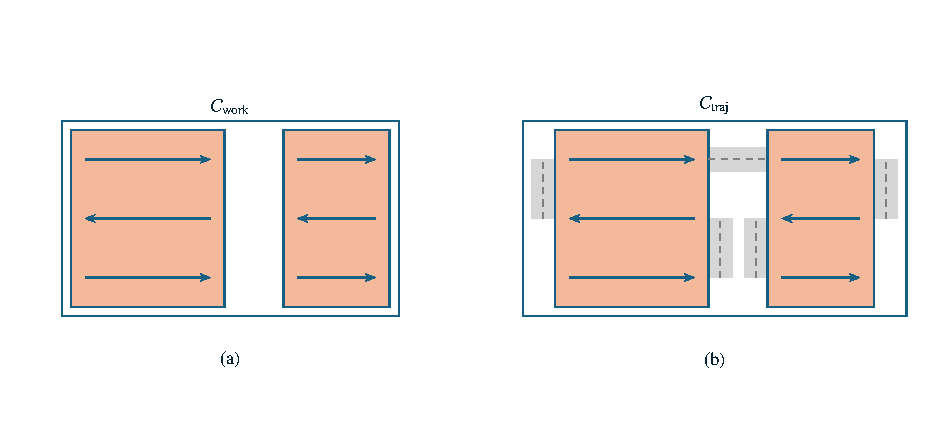
\includegraphics[width=0.92\linewidth]{figures/figure_coverage_segments.pdf}}}\\[0.25em]
{\color{blue}\scriptsize 新增}
% ===FIGNEW END figure_coverage_segments.png===
  \caption{\DIFaddFL{Work coverage counts disc sweeps on work strips; full-trajectory coverage also counts sweeps during transfer and adjustment.}}
  \label{fig:coverage-segments}
\end{figure}\marginpar{\scriptsize [67] 用两个矩形和一次转移新画覆盖率原理图，未用实验地图。}

\DIFaddend For any segment $s$, let the disc-center path be
\begin{equation}
\mathbf p_d^s(\tau),\qquad \tau\in[0,T_s].
\tag{23}
\label{eq:segment-center}
\end{equation}
The disc-swept region of the segment is
\begin{equation}
\mathcal C_s=\bigcup_{\tau\in[0,T_s]}\left\{\mathbf z:\|\mathbf z-\mathbf p_d^s(\tau)\|_2\le r_d\right\}.
\tag{24}
\label{eq:segment-sweep}
\end{equation}

Let $\mathcal S_{\mathrm{work}}$ be the set of effective-work segments and $\mathcal S_{\mathrm{all}}$ the set of all motion segments. The method distinguishes
\begin{equation}
\mathcal C_{\mathrm{work}}=\bigcup_{s\in\mathcal S_{\mathrm{work}}}\mathcal C_s,
\qquad
\mathcal C_{\mathrm{traj}}=\bigcup_{s\in\mathcal S_{\mathrm{all}}}\mathcal C_s.
\tag{25}
\label{eq:work-and-trajectory-sweeps}
\end{equation}
The former contains only work-labeled disc sweeps, whereas the latter also includes disc motion during transfer, lane changes, and pose adjustment. Their respective coverage ratios are
\begin{equation}
\begin{aligned}
\rho_{\mathrm{work}}&=\frac{|\Pi_p(\mathcal C_{\mathrm{work}})\cap\mathcal P_F|}{|\mathcal P_F|},\\
\rho_{\mathrm{traj}}&=\frac{|\Pi_p(\mathcal C_{\mathrm{traj}})\cap\mathcal P_F|}{|\mathcal P_F|},
\end{aligned}
\tag{26}
\label{eq:coverage-ratios}
\end{equation}
where $\Pi_p(\cdot)$ rasterizes a continuous world-coordinate region into a pixel set. The primary coverage measure is $\rho_{\mathrm{work}}$ because it corresponds to explicitly labeled effective-work motion. The value $\rho_{\mathrm{traj}}$ describes how much free area is swept over the complete motion. If the disc remains in contact with the floor during non-working transfers, it captures additional physical sweeping; if the disc is lifted, it is only an auxiliary measure of path reach or potential sweep and must not be conflated with effective work coverage.

To avoid dependence on an arbitrary sampling frame rate, $\mathbf p_d^s(\tau)$ is recursively subdivided. A time interval $[\tau_a,\tau_b]$ is accepted only when the endpoint chord length is no greater than $\eta_\ell$ and the deviation of the midpoint from that chord is no greater than $\eta_c$. Both are chosen no larger than $s_p/2$, bounding discretization error by map resolution. Let the final subdivision points be $\mathbf c_0,\ldots,\mathbf c_m$. Rasterizing the radius-$r_d$ capsule between every adjacent pair yields
\begin{equation}
\widehat{\mathcal C}_s=\Pi_p\!\left(\bigcup_{j=0}^{m-1}\mathrm{Capsule}(\mathbf c_j,\mathbf c_{j+1},r_d)\right).
\tag{27}
\label{eq:rasterized-sweep}
\end{equation}
The capsule union is constructed in world coordinates before conversion by $\Pi_p$, avoiding a type mismatch between continuous regions and pixel sets. This method is more stable than drawing discs only at fixed-rate samples, especially during fast arm motion.

Finally, nominal execution time and planning time are
\begin{equation}
T_{\mathrm{exec}}=\sum_{s\in\mathcal S_{\mathrm{all}}}T_s,
\qquad
T_{\mathrm{plan}}=t_{\mathrm{eval,end}}-t_{\mathrm{raster,start}}.
\tag{28}
\label{eq:timing-measures}
\end{equation}
The first follows the piecewise-constant and serial-timing assumptions used for the local primitives. The second is measured as wall-clock time in one process, from conservative-grid generation through continuous-sweep evaluation. It includes decomposition, connectivity completion, route search, trajectory assembly, and coverage computation, but excludes map-file reading, output writing, and visualization. Thus $\rho_{\mathrm{work}}$, $\rho_{\mathrm{traj}}$, $T_{\mathrm{exec}}$, and $T_{\mathrm{plan}}$ match the output definitions in Fig.~\ref{fig:pipeline}.

\section{Experiments and Results}
\label{sec:experiments}

Three groups of experiments \DIFaddbegin \DIFadd{are designed to }\marginpar{\scriptsize [68] 在实验与评估两个动词之间补上表示设计目的的系动词。}\DIFaddend evaluate the proposed swing-arm CPP method. The first compares \DIFdelbegin \DIFdel{it }\DIFdelend \DIFaddbegin \DIFadd{BiRect }\DIFaddend with Fields2Cover to \DIFdelbegin \DIFdel{clarify the difference between active arm sweeping and }\DIFdelend \DIFaddbegin \DIFadd{verify that, on obstacle maps, active swing-arm motion gives executable coverage and a higher full-trajectory coverage ratio than }\marginpar{\scriptsize [69] 将第一组实验改为验证可执行覆盖和更高的全程覆盖率。}\DIFaddend fixed-width \DIFdelbegin \DIFdel{strip-based CPP}\DIFdelend \DIFaddbegin \DIFadd{strips}\DIFaddend . The second compares rectangular-candidate scan strategies to determine how \DIFdelbegin \DIFdel{decomposition affects }\DIFdelend \DIFaddbegin \DIFadd{bidirectional candidates affect }\DIFaddend coverage quality and redundancy in complex spaces. The third varies base speed at a fixed arm angular velocity to expose how \DIFdelbegin \DIFdel{velocity matching }\DIFdelend \DIFaddbegin \DIFadd{base--arm velocity coupling }\DIFaddend affects coverage and execution time.

All three groups use two base maps. \texttt{\DIFdelbegin \DIFdel{map\_test1}\DIFdelend \DIFaddbegin \DIFadd{simple}\DIFaddend } contains four regular rectangular obstacles and tests basic obstacle avoidance and coverage. \texttt{\DIFdelbegin \DIFdel{parkingGraph}\DIFdelend \DIFaddbegin \DIFadd{complex}\DIFaddend } contains densely distributed small obstacles and better resembles a construction floor partitioned by columns, openings, and local structures. The scan-strategy experiment additionally uses three directional maps:
\begin{itemize}[nosep]
  \item \texttt{scan\_comb\_corridors}: horizontal comb-like corridors;
  \item \texttt{scan\_mixed\_weave}: interwoven horizontal and vertical structures; and
  \item \texttt{scan\_offset\_rooms}: rooms connected with offsets.
\end{itemize}
These structures distinguish the effects of row-only, column-only, and bidirectional scanning.

Every map is a binary occupancy image\DIFdelbegin \DIFdel{in which white pixels are free target area and black pixels are obstacles or unavailable regions}\DIFdelend \DIFaddbegin \DIFadd{, with free and unavailable pixels as defined above}\marginpar{\scriptsize [71] 将黑白像素的重复定义改为一句，改按前文定义。}\DIFaddend . The resolution is $0.5$~m/pixel. Except in the speed experiment, the same parameters are used throughout: disc radius $r_d=0.75$~m, arm length $L=1.20$~m, base width $0.80$~m, maximum base linear velocity $2.00$~m/s, maximum base angular velocity $30^\circ$/s, and maximum arm angular velocity $90^\circ$/s. \DIFdelbegin \DIFdel{The }\DIFdelend \DIFaddbegin \DIFadd{Outside the speed experiment these three limits are used together. The actual work speed is still $v_{\mathrm{work}}=\min(v_{\max},v_{\mathrm{safe}})$ from Section~3.5.3, so the limits are not the travel speed of every strip. In the speed experiment the arm angular velocity stays $90^\circ$/s and the base angular velocity stays $30^\circ$/s, while the base linear velocity takes the six values $0.5$, $1.0$, $1.5$, $2.0$, $2.5$, and $3.0$~m/s. The }\marginpar{\scriptsize [72] 写明已有速度组合，未新跑实验，也未增加臂角速度扫描。}\DIFaddend minimum rectangle side length is $2.5$~m, the greedy-selection weights are $\alpha=0.5$ and $\beta=2.0$, and the random seed is 42.

\subsection{\DIFdelbegin \DIFdel{Comparison with }\DIFdelend \DIFaddbegin \DIFadd{Executability and Coverage against }\DIFaddend Fields2Cover}\marginpar{\scriptsize [73] 将实验小节标题改为 Executability and Coverage against Fields2Cover。}

Fields2Cover is \DIFdelbegin \DIFdel{an appropriate }\DIFdelend \DIFaddbegin \DIFadd{the }\DIFaddend fixed-width \DIFdelbegin \DIFdel{baseline and a representative open-source framework for this class of problem. It is supported by a peer-reviewed publication and continuing open-source development, integrates multiple coverage-planning algorithms and objectives, and includes headland generation, swath generation, route ordering, and curvature-constrained path connections. It supports non-convex regions, internal obstacles, fixed working and vehicle widths, turning radii, and speed parameters. Its functional completeness, algorithmic integration, and reproducibility make it a strong contemporary baseline for fixed-width CPP \mbox{%DIFAUXCMD
\cite{mier2023,fields2cover}}\hskip0pt%DIFAUXCMD
. The comparison is not intended to rank implementation details, but to expose differences in coverage geometry and executability between an active swing-arm model and an integrated, fixed-width strip-planning framework in obstacle-rich spaces}\marginpar{\scriptsize [74] 删去实验节中 Fields2Cover 的功能介绍，只保留对照设置。}\DIFdelend \DIFaddbegin \DIFadd{representative from Section~\ref{sec:related-work}, and it is used here to verify executable coverage and a higher full-trajectory coverage ratio}\DIFaddend .

For Fields2Cover, the working width is $1.50$~m, equal to the diameter of the proposed method's $0.75$~m-radius disc. With base width $0.80$~m and safety margin $0.05$~m, the original free region is eroded by $0.45$~m. Both methods are evaluated over their complete trajectories. For the proposed method, coverage is the area swept by the disc along the base--arm trajectory; for Fields2Cover, it is the fixed-width tool sweep along work, turning, and transfer segments. To align evaluation with the actual planning domain, the Fields2Cover denominator is the eroded free-space area. Its fixed-width sweep uses flat strip ends and mitered path corners. The work-strip speed is $2.0$~m/s, while turns and connecting paths use $0.5$~m/s.

\DIFaddbegin \begin{figure}[H]
  \centering
  % ===FIGPAIR figure_2_coverage_comparison_en.png===
\par\noindent\begin{minipage}[t]{0.48\linewidth}\centering
{\setlength{\fboxsep}{1.2pt}\setlength{\fboxrule}{1.1pt}%
\fcolorbox{red}{white}{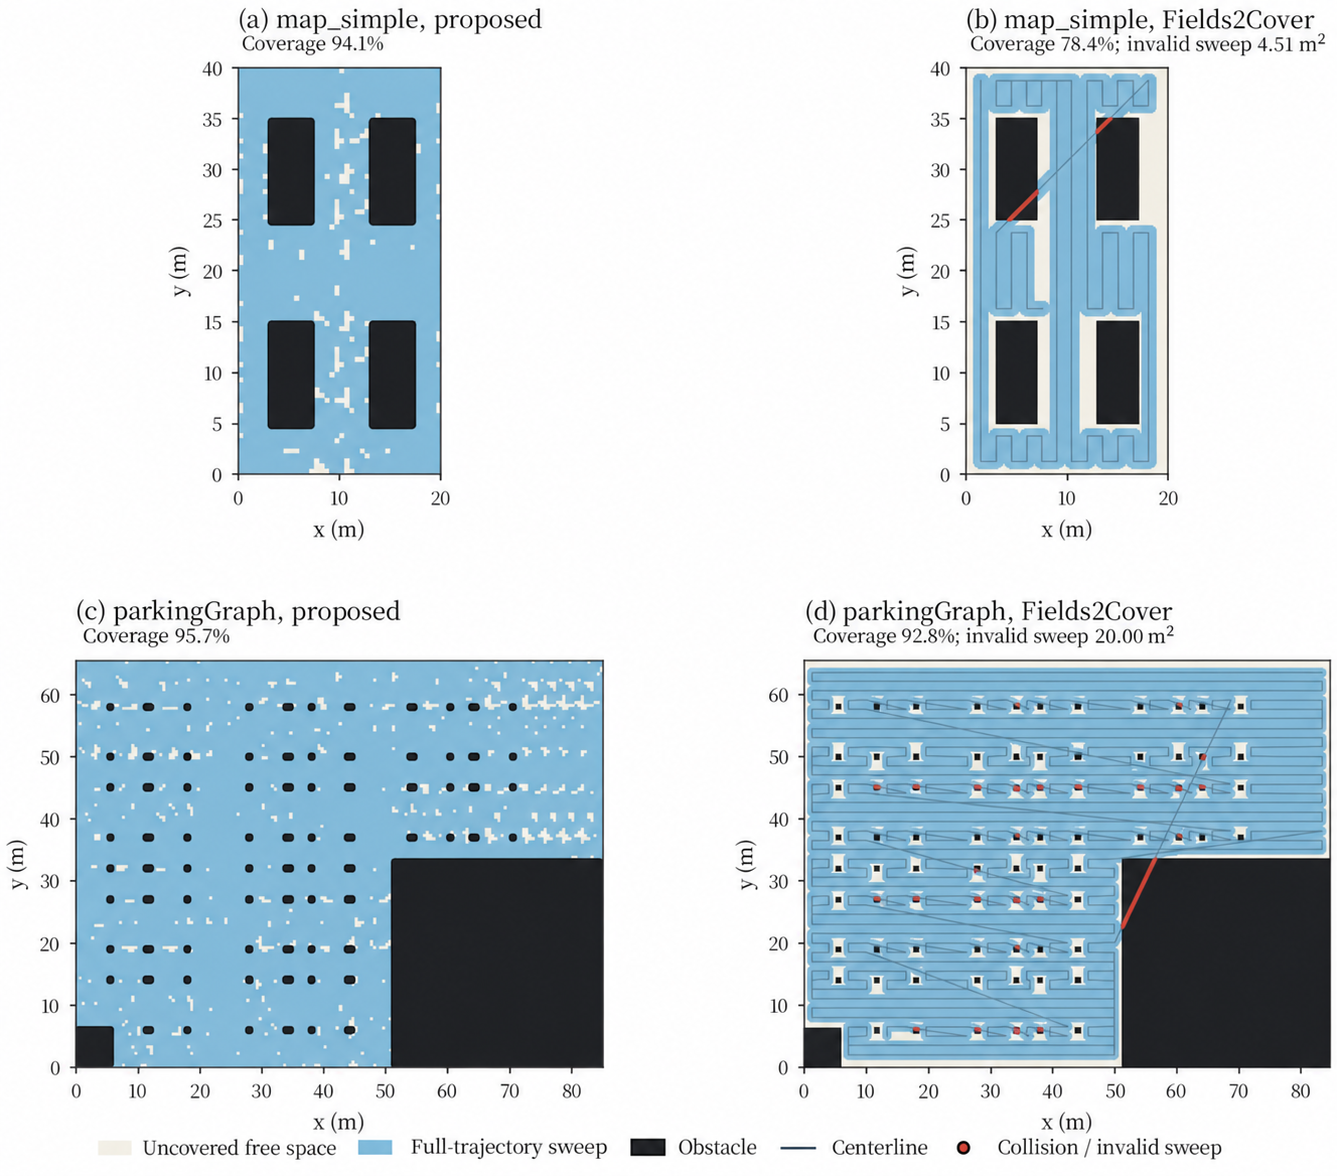
\includegraphics[width=\dimexpr\linewidth-2\fboxsep-2\fboxrule\relax]{old_figs/figure_2_coverage_comparison_en.png}}}\\[0.25em]
{\color{red}\scriptsize 修改前}
\end{minipage}\hfill
\begin{minipage}[t]{0.48\linewidth}\centering
{\setlength{\fboxsep}{1.2pt}\setlength{\fboxrule}{1.1pt}%
\fcolorbox{blue}{white}{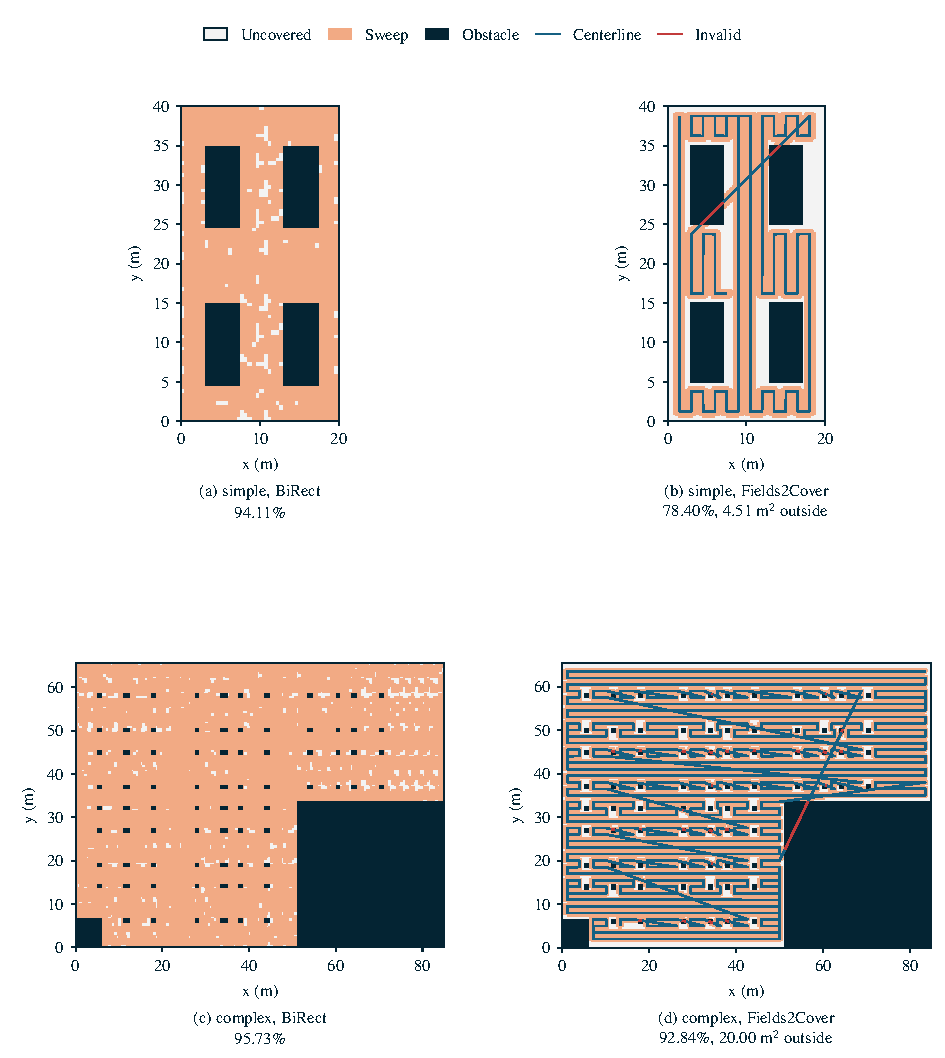
\includegraphics[width=\dimexpr\linewidth-2\fboxsep-2\fboxrule\relax]{figures/figure_2_coverage_comparison_en.pdf}}}\\[0.25em]
{\color{blue}\scriptsize 修改后}
\end{minipage}\par
% ===FIGPAIR END figure_2_coverage_comparison_en.png===
  \caption{\DIFaddFL{Coverage paths and swept regions for the proposed method and Fields2Cover: panels (a) and (b) show }\texttt{\DIFaddFL{simple}}\DIFaddFL{, and panels (c) and (d) show }\texttt{\DIFaddFL{complex}}\DIFaddFL{.}}
  \label{fig:baseline-comparison}
\end{figure}\marginpar{\scriptsize [70] 把正文和图中的地图名改为 simple 与 complex，数字和数据文件未改。}\marginpar{\scriptsize [79] 将覆盖对比图移到实验介绍之后，并固定浮动位置。}

\DIFaddend \begin{table}[htbp]
\centering
\caption{Comparison between the proposed method and Fields2Cover.}
\label{tab:baseline-comparison}
\scriptsize
\setlength{\tabcolsep}{3pt}
\renewcommand{\arraystretch}{1.18}
\begin{tabular}{@{}p{1.95cm}p{1.45cm}rrrrp{2.55cm}@{}}
\toprule
Map & Method & \shortstack{Evaluation\\area (m$^2$)} & \shortstack{Covered\\area (m$^2$)} & \shortstack{Coverage\\ratio (\%)} & \shortstack{Execution/planning\\time (s/s)} & Path check \\
\midrule
\texttt{\DIFdelbeginFL \DIFdelFL{map\_test1}\DIFdelendFL \DIFaddbeginFL \DIFaddFL{simple}\DIFaddendFL } & \DIFdelbeginFL \DIFdelFL{Proposed }\DIFdelendFL \DIFaddbeginFL \textbf{\DIFaddFL{BiRect}} \DIFaddendFL & 611.00 & 575.00 & \DIFdelbeginFL \DIFdelFL{94.11 }\DIFdelendFL \DIFaddbeginFL \textbf{\DIFaddFL{94.11}} \DIFaddendFL & 854.73/1.298 & \DIFdelbeginFL \DIFdelFL{Passed }\DIFdelendFL \DIFaddbeginFL \textbf{\DIFaddFL{Passed}} \DIFaddendFL \\
 & Fields2Cover & 533.17 & 418.00 & 78.40 & 295.50/0.075 & 4.51~m$^2$ outside \\
\texttt{\DIFdelbeginFL \DIFdelFL{parking}\DIFdelendFL \DIFaddbeginFL \DIFaddFL{complex}\DIFaddendFL } \DIFdelbeginFL %DIFDELCMD < \allowbreak%%%
\texttt{\DIFdelFL{Graph}} %DIFAUXCMD
\DIFdelendFL & \DIFdelbeginFL \DIFdelFL{Proposed }\DIFdelendFL \DIFaddbeginFL \textbf{\DIFaddFL{BiRect}} \DIFaddendFL & 4294.00 & 4110.50 & \DIFdelbeginFL \DIFdelFL{95.73 }\DIFdelendFL \DIFaddbeginFL \textbf{\DIFaddFL{95.73}} \DIFaddendFL & 5844.73/17.981 & \DIFdelbeginFL \DIFdelFL{Passed }\DIFdelendFL \DIFaddbeginFL \textbf{\DIFaddFL{Passed}} \DIFaddendFL \\
 & Fields2Cover & 4046.79 & 3756.85 & 92.84 & 2883.81/6.339 & 20.00~m$^2$ outside \\
\bottomrule
\end{tabular}
\end{table}\marginpar{\scriptsize [75] 把表中方法名改为 BiRect，并加粗其占优的覆盖率和 Passed，数字未改。}

The evaluated areas in Table~\ref{tab:baseline-comparison} differ between methods, so their coverage ratios should not be interpreted as same-domain percentage-point differences. The Fields2Cover routes fail the path check; their execution and planning times are reported only for the generated outputs.

On \texttt{\DIFdelbegin \DIFdel{map\_test1}\DIFdelend \DIFaddbegin \DIFadd{simple}\DIFaddend }, Fields2Cover has shorter generation and nominal execution times with a $1.50$~m fixed width equal to the disc diameter. Its complete trajectory sweeps 418.00~m$^2$ (78.40\%), compared with 575.00~m$^2$ (94.11\%) for the proposed method. Its connecting segments, however, sweep 4.51~m$^2$ outside the admissible region. The recorded 295.50~s execution time and 0.075~s planning time therefore describe an invalid generated path rather than an executable solution. This illustrates the principal benefit of the swing-arm configuration: the base need not drive along every strip that the disc must cover. Arm motion extends the covered region and creates a wider time-varying sweep within the same free space.

On \texttt{\DIFdelbegin \DIFdel{parkingGraph}\DIFdelend \DIFaddbegin \DIFadd{complex}\DIFaddend }, the proposed method covers 4110.50~m$^2$, or 95.73\% of its evaluation domain. Fields2Cover sweeps 3756.85~m$^2$ (92.84\%) along the complete trajectory. Yet its connecting path for the $1.50$~m tool leaves the free space, creating 20.00~m$^2$ of invalid base sweep; the corresponding 2883.81~s execution time and 6.339~s planning time are likewise not valid baseline scores. The problem is concentrated near dense local obstacles. Although individual swaths fit inside the eroded region, curvature-constrained connections between swaths require additional room. Without a broad transfer area analogous to an agricultural headland, these connections can cross the boundary of the original free space. Active arm sweeping partially decouples base travel from end-disc coverage and preserves greater coverage capability and path continuity in such complex regions.

\DIFdelbegin %DIFDELCMD < \begin{figure}[htbp]
%DIFDELCMD <   \centering
%DIFDELCMD <   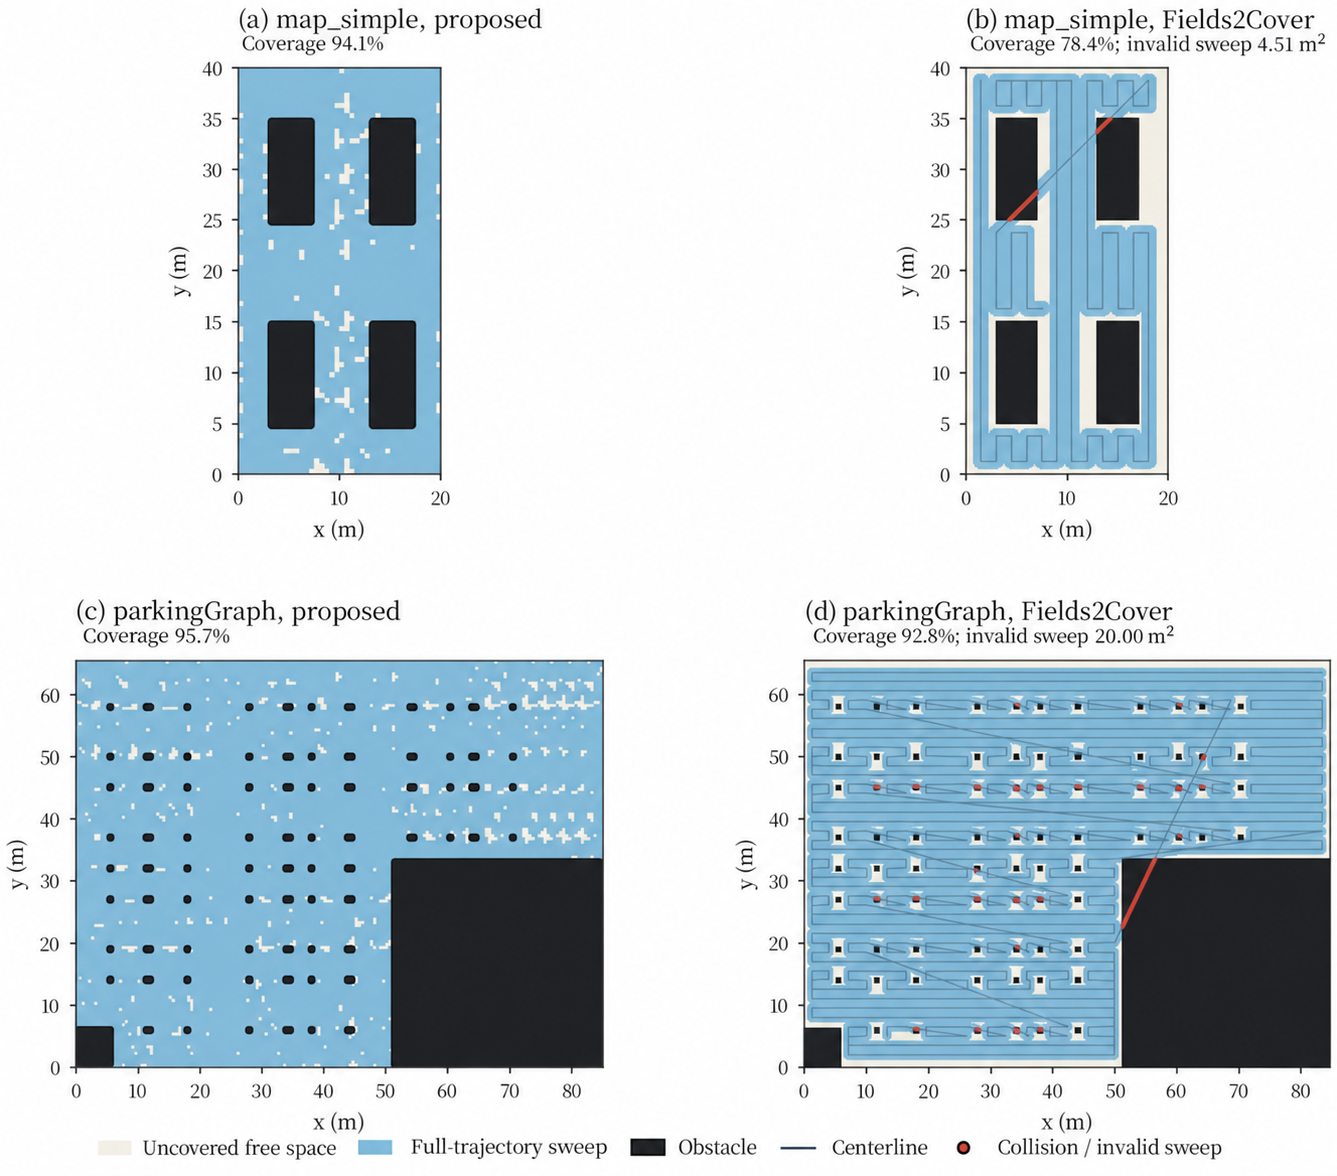
\includegraphics[width=0.96\linewidth]{figure_2_coverage_comparison_en.png}
%DIFDELCMD <   %%%
%DIFDELCMD < \caption{%
{%DIFAUXCMD
\DIFdelFL{Coverage paths and swept regions for the proposed method and Fields2Cover. Panels (a) and (b) show }\texttt{\DIFdelFL{map\_test1}} %DIFAUXCMD
\DIFdelFL{(labeled }\texttt{\DIFdelFL{map\_simple}} %DIFAUXCMD
\DIFdelFL{inside the image), and panels (c) and (d) show }\texttt{\DIFdelFL{parkingGraph}}%DIFAUXCMD
\DIFdelFL{; the proposed method is on the left and Fields2Cover on the right. Blue is the full-trajectory swept region, white or light areas are uncovered free space in the evaluation domain, black is obstacle or unavailable space, and red marks base collisions or invalid sweep. The Fields2Cover route fails the base-collision check on both maps: 4.51~m\mbox{$^2$} lies outside the valid region on }\texttt{\DIFdelFL{map\_test1}} %DIFAUXCMD
\DIFdelFL{and 20.00~m\mbox{$^2$} on }\texttt{\DIFdelFL{parkingGraph}}%DIFAUXCMD
\DIFdelFL{. Its displayed coverage and timing values therefore describe generated, non-executable routes.}}
  %DIFAUXCMD
%DIFDELCMD < \label{fig:baseline-comparison}
%DIFDELCMD < \end{figure}
%DIFDELCMD < 

%DIFDELCMD < %%%
\DIFdelend \subsection{Effect of the Rectangle-Candidate Scan Strategy}

The preceding comparison shows that an active arm can create coverage patterns unlike those of fixed-width strips. Realizing this advantage consistently also requires a decomposition that represents free space appropriately. A candidate generator biased toward one scan direction can produce fragmented or heavily overlapping rectangles; even when the resulting trajectory is executable, unnecessary transfers may follow. This experiment traces how scan direction propagates through the rectangle set, visitation sequence, and complete trajectory.

The compared strategies are row-only, column-only, and row-then-column scanning. Robot parameters, minimum rectangle size, greedy weights, random seed, connectivity completion, visitation ordering, and local coverage generation are fixed. Measures include greedy coverage, final decomposition coverage, decomposition overlap, full-trajectory coverage, and total execution time, distinguishing representation quality from execution performance. Candidates are first generated and greedily selected from a binary map. After hole filling and connectivity completion, the same trajectory generation and disc-sweep evaluation method is applied in every case.

\DIFdelbegin %DIFDELCMD < \begin{longtable}{@{}p{2.50cm}p{1.60cm}>{\raggedleft\arraybackslash}p{1.55cm}>{\raggedleft\arraybackslash}p{1.65cm}>{\raggedleft\arraybackslash}p{1.45cm}>{\raggedleft\arraybackslash}p{1.60cm}>{\raggedleft\arraybackslash}p{1.55cm}@{}}
%DIFDELCMD < %%%
\DIFdelend \DIFaddbegin \begin{longtable}{@{}p{2.50cm}p{2.50cm}>{\raggedleft\arraybackslash}p{1.55cm}>{\raggedleft\arraybackslash}p{1.65cm}>{\raggedleft\arraybackslash}p{1.45cm}>{\raggedleft\arraybackslash}p{1.60cm}>{\raggedleft\arraybackslash}p{1.55cm}@{}}
\DIFaddend \caption{Results of three candidate-scan strategies on five maps.}\label{tab:scan-strategy}\\
\toprule
Map & Strategy & \shortstack{Greedy\\coverage} & \shortstack{Final\\partition\\coverage} & \shortstack{Partition\\overlap} & \shortstack{Trajectory\\coverage} & \shortstack{Total time\\(s)} \\
\midrule
\endfirsthead
\toprule
Map & Strategy & \shortstack{Greedy\\coverage} & \shortstack{Final\\partition\\coverage} & \shortstack{Partition\\overlap} & \shortstack{Trajectory\\coverage} & \shortstack{Total time\\(s)} \\
\midrule
\endhead
\texttt{\DIFdelbegin \DIFdel{map\_test1}\DIFdelend \DIFaddbegin \DIFadd{simple}\DIFaddend } & \DIFdelbegin \DIFdel{row-only }\DIFdelend \DIFaddbegin \textbf{\DIFadd{row-only}} \DIFaddend & 72.01\% & 100.00\% & 34.21\% & 93.04\% & \DIFdelbegin \DIFdel{696.89 }\DIFdelend \DIFaddbegin \textbf{\DIFadd{696.89}} \DIFaddend \\
 & \DIFdelbegin \DIFdel{col-only }\DIFdelend \DIFaddbegin \textbf{\DIFadd{col-only}} \DIFaddend & 72.01\% & 100.00\% & 34.21\% & 93.04\% & \DIFdelbegin \DIFdel{696.89 }\DIFdelend \DIFaddbegin \textbf{\DIFadd{696.89}} \DIFaddend \\
 & \DIFdelbegin \DIFdel{row-then-col }\DIFdelend \DIFaddbegin \textbf{\DIFadd{\mbox{row-then-col}}} \DIFaddend & \DIFdelbegin \DIFdel{100.00\% }\DIFdelend \DIFaddbegin \textbf{\DIFadd{100.00\%}} \DIFaddend & 100.00\% & \DIFdelbegin \DIFdel{0.00\% }\DIFdelend \DIFaddbegin \textbf{\DIFadd{0.00\%}} \DIFaddend & \DIFdelbegin \DIFdel{94.11\% }\DIFdelend \DIFaddbegin \textbf{\DIFadd{94.11\%}} \DIFaddend & 854.73 \\
\midrule
\texttt{\DIFdelbegin \DIFdel{parking}\DIFdelend \DIFaddbegin \DIFadd{complex}\DIFaddend } \DIFdelbegin %DIFDELCMD < \allowbreak%%%
\texttt{\DIFdel{Graph}} %DIFAUXCMD
\DIFdelend & \DIFdelbegin \DIFdel{row-only }\DIFdelend \DIFaddbegin \textbf{\DIFadd{row-only}} \DIFaddend & 87.32\% & 100.00\% & 75.34\% & 95.73\% & \DIFdelbegin \DIFdel{5844.73 }\DIFdelend \DIFaddbegin \textbf{\DIFadd{5844.73}} \DIFaddend \\
 & \DIFdelbegin \DIFdel{col-only }\DIFdelend \DIFaddbegin \textbf{\DIFadd{col-only}} \DIFaddend & 87.32\% & 100.00\% & 75.34\% & \DIFdelbegin \DIFdel{95.90\% }\DIFdelend \DIFaddbegin \textbf{\DIFadd{95.90\%}} \DIFaddend & 5896.03 \\
 & \DIFdelbegin \DIFdel{row-then-col }\DIFdelend \DIFaddbegin \textbf{\DIFadd{\mbox{row-then-col}}} \DIFaddend & 87.32\% & 100.00\% & 75.34\% & 95.73\% & \DIFdelbegin \DIFdel{5844.73 }\DIFdelend \DIFaddbegin \textbf{\DIFadd{5844.73}} \DIFaddend \\
\midrule
Comb corridors & row-only & 87.18\% & 100.00\% & 34.46\% & 93.82\% & 2065.09 \\
 & col-only & 86.53\% & 100.00\% & 31.46\% & 93.94\% & 2032.55 \\
 & \DIFdelbegin \DIFdel{row-then-col }\DIFdelend \DIFaddbegin \textbf{\DIFadd{\mbox{row-then-col}}} \DIFaddend & \DIFdelbegin \DIFdel{96.22\% }\DIFdelend \DIFaddbegin \textbf{\DIFadd{96.22\%}} \DIFaddend & 100.00\% & \DIFdelbegin \DIFdel{27.13\% }\DIFdelend \DIFaddbegin \textbf{\DIFadd{27.13\%}} \DIFaddend & \DIFdelbegin \DIFdel{94.01\% }\DIFdelend \DIFaddbegin \textbf{\DIFadd{94.01\%}} \DIFaddend & \DIFdelbegin \DIFdel{1986.42 }\DIFdelend \DIFaddbegin \textbf{\DIFadd{1986.42}} \DIFaddend \\
\midrule
Mixed weave & row-only & 84.23\% & 100.00\% & 47.89\% & 95.26\% & 1532.65 \\
 & col-only & 83.17\% & 100.00\% & 52.59\% & 95.49\% & 1575.63 \\
 & \DIFdelbegin \DIFdel{row-then-col }\DIFdelend \DIFaddbegin \textbf{\DIFadd{\mbox{row-then-col}}} \DIFaddend & \DIFdelbegin \DIFdel{96.76\% }\DIFdelend \DIFaddbegin \textbf{\DIFadd{96.76\%}} \DIFaddend & 100.00\% & \DIFdelbegin \DIFdel{40.74\% }\DIFdelend \DIFaddbegin \textbf{\DIFadd{40.74\%}} \DIFaddend & \DIFdelbegin \DIFdel{95.70\% }\DIFdelend \DIFaddbegin \textbf{\DIFadd{95.70\%}} \DIFaddend & \DIFdelbegin \DIFdel{1522.77 }\DIFdelend \DIFaddbegin \textbf{\DIFadd{1522.77}} \DIFaddend \\
\midrule
Offset rooms & row-only & 82.95\% & 100.00\% & 38.78\% & 91.97\% & 1496.73 \\
 & col-only & 81.81\% & 100.00\% & 36.74\% & 91.51\% & 1443.31 \\
 & \DIFdelbegin \DIFdel{row-then-col }\DIFdelend \DIFaddbegin \textbf{\DIFadd{\mbox{row-then-col}}} \DIFaddend & \DIFdelbegin \DIFdel{99.14\% }\DIFdelend \DIFaddbegin \textbf{\DIFadd{99.14\%}} \DIFaddend & 100.00\% & \DIFdelbegin \DIFdel{24.46\% }\DIFdelend \DIFaddbegin \textbf{\DIFadd{24.46\%}} \DIFaddend & \DIFdelbegin \DIFdel{92.06\% }\DIFdelend \DIFaddbegin \textbf{\DIFadd{92.06\%}} \DIFaddend & \DIFdelbegin \DIFdel{1374.38 }\DIFdelend \DIFaddbegin \textbf{\DIFadd{1374.38}} \DIFaddend \\
\midrule
Five-map mean & row-only & -- & -- & -- & 93.96\% & 2327.22 \\
 & col-only & -- & -- & -- & 93.98\% & 2328.88 \\
 & \DIFdelbegin \DIFdel{row-then-col }\DIFdelend \DIFaddbegin \textbf{\DIFadd{\mbox{row-then-col}}} \DIFaddend & -- & -- & -- & \DIFdelbegin \DIFdel{94.32\% }\DIFdelend \DIFaddbegin \textbf{\DIFadd{94.32\%}} \DIFaddend & \DIFdelbegin \DIFdel{2316.60 }\DIFdelend \DIFaddbegin \textbf{\DIFadd{2316.60}} \DIFaddend \\
\bottomrule
\end{longtable}\marginpar{\scriptsize [76] 按列加粗扫描策略表中的占优格子，并避免策略名拆行，数字未改。}

The two general maps first establish basic behavior in non-directional scenes.\linebreak On \texttt{\DIFdelbegin \DIFdel{map\_test1}\DIFdelend \DIFaddbegin \DIFadd{simple}\DIFaddend }, row-then-column achieves the highest full-trajectory coverage (94.11\%) and reduces partition overlap to zero, but its 854.73~s execution time exceeds the 696.89~s of either one-direction strategy. In this regular obstacle scene, bidirectional scanning trades longer execution for higher coverage. On \texttt{\DIFdelbegin \DIFdel{parkingGraph}\DIFdelend \DIFaddbegin \DIFadd{complex}\DIFaddend }, row-then-column and row-only select the same rectangles and give identical results. Column-only provides slightly higher coverage (95.90\%), whereas row-only and row-then-column tie for the shortest total time (5844.73~s). Bidirectional scanning therefore does not dominate every metric in every scene. When free space has a pronounced principal direction or row candidates already capture the structure, a one-direction strategy may be faster or marginally improve coverage.

The three directional maps then isolate scan-direction bias; they are not intended to prove that bidirectional scanning is optimal on arbitrary maps. Horizontal corridors, orthogonal interweaving, and offset connections amplify residual regions created by a single scan direction. On all three maps, row-then-column gives the highest greedy coverage and lowest partition overlap. Column candidates supplement regions that row candidates represent poorly rather than merely increasing the rectangle count. This improvement propagates to execution: row-then-column gives both the highest full-trajectory coverage and shortest time on all three maps, respectively 94.01\%/1986.42~s, 95.70\%/1522.77~s, and 92.06\%/1374.38~s. Their mean is 93.93\%/1627.86~s. When a map truly contains residual structures in both directions, complementary row and column candidates reduce directional bias and redundant visitation while increasing useful sweep along the complete trajectory.

Across \DIFdelbegin \DIFdel{all }\DIFdelend \DIFaddbegin \DIFadd{the }\DIFaddend five maps, \DIFdelbegin \DIFdel{row-then-column averages }\DIFdelend \DIFaddbegin \DIFadd{the arithmetic mean of full-trajectory coverage is }\marginpar{\scriptsize [77] 将该百分比写成五张图全程覆盖率的算术平均，数字未改。}\DIFaddend 94.32\% \DIFdelbegin \DIFdel{coverage, compared with }\DIFdelend \DIFaddbegin \DIFadd{for row-then-column, }\DIFaddend 93.96\% for row-only\DIFaddbegin \DIFadd{, }\DIFaddend and 93.98\% for column-only. Its mean execution time of 2316.60~s is also slightly below 2327.22~s and 2328.88~s. It is therefore best characterized as a robust default: it is more likely to preserve high coverage without a substantial time penalty when horizontal and vertical residual structures coexist. For a regular region with a single principal direction, a one-direction strategy may still be preferable under the specific coverage--schedule trade-off. Figure~\ref{fig:scan-strategy} visualizes the directional complementarity on \texttt{scan\_mixed\_weave}.

\begin{figure}[htbp]
  \centering
  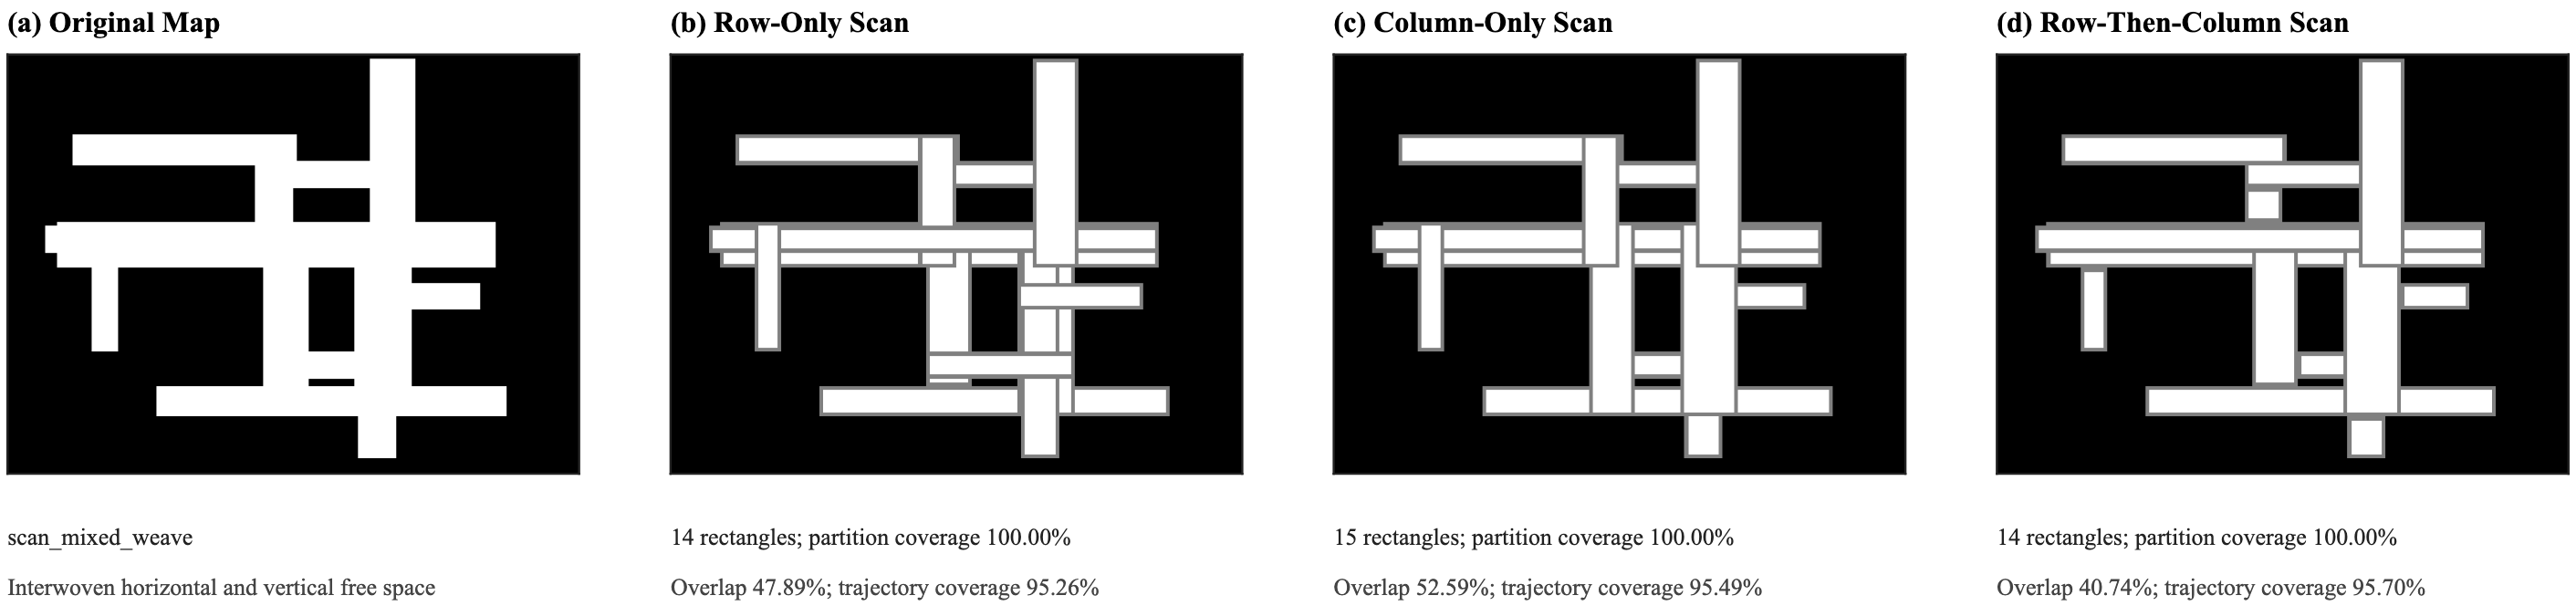
\includegraphics[width=0.96\linewidth]{figure_3_segmentation_order_en.png}
  \caption{Candidate-scan strategies on \texttt{scan\_mixed\_weave}: (a) original map; (b) row-only decomposition; (c) column-only decomposition; and (d) row-then-column decomposition.\DIFdelbeginFL \DIFdelFL{The map contains narrow horizontal and vertical free regions. Single-direction candidate sets leave residual structures in the other orientation, whereas sequential row and column candidates form a more complete decomposition with less overlap.}\DIFdelendFL }
  \label{fig:scan-strategy}
\end{figure}

\subsection{Effect of Base--Arm Velocity Coupling on Coverage}

The first two experiments address route and decomposition quality. Swing-arm coverage also has an execution issue that is less prominent in fixed-width CPP: the same geometric route produces different disc-sweep densities at different base speeds. As the base advances faster, it travels farther between adjacent arm sweeps; slower travel improves coverage but substantially increases task time. Reporting a geometric \DIFdelbegin \DIFdel{path without analyzing its velocity relationship to the arm }\DIFdelend \DIFaddbegin \DIFadd{route without analyzing base--arm velocity coupling }\DIFaddend therefore cannot establish the coverage quality and time cost of actual execution.

This experiment tests the analysis in Section~3.5.3. At fixed arm angular velocity, increasing base speed should shorten execution but enlarge the spacing between adjacent sweeps and reduce coverage. Keeping the rectangle set, visitation order, and local-work structure fixed isolates the effect of base speed.

The arm angular velocity is fixed at $\omega_a=90^\circ$/s. The same planned solutions are executed on \texttt{\DIFdelbegin \DIFdel{map\_test1}\DIFdelend \DIFaddbegin \DIFadd{simple}\DIFaddend } and \texttt{\DIFdelbegin \DIFdel{parkingGraph}\DIFdelend \DIFaddbegin \DIFadd{complex}\DIFaddend } with base speed increasing from 0.5 to 3.0~m/s. \DIFdelbegin \DIFdel{A velocity ratio places linear and angular speed on a common scale:
}\DIFdelend \DIFaddbegin \DIFadd{The ratio of this base--arm velocity coupling is
}\marginpar{\scriptsize [78] 统一称为 base–arm velocity coupling，速度比只作为该耦合的比值。}\DIFaddend \begin{equation*}
\rho=\frac{v}{\omega_a},
\end{equation*}
with units of m/degree. It is the base distance traveled while the arm rotates through $1^\circ$. A larger $\rho$ increases forward spacing between adjacent sweeps and makes coverage gaps more likely. Coverage, total time, and time per unit covered area are recorded to expose the quality--efficiency trade-off.

\begin{table}[htbp]
\centering
\caption{Full-trajectory coverage and execution time at different base speeds.}
\label{tab:speed-study}
\scriptsize
\setlength{\tabcolsep}{3pt}
\renewcommand{\arraystretch}{1.12}
\begin{tabular}{@{}p{2.15cm}>{\raggedleft\arraybackslash}p{1.35cm}>{\raggedleft\arraybackslash}p{1.7cm}>{\raggedleft\arraybackslash}p{1.9cm}>{\raggedleft\arraybackslash}p{1.7cm}>{\raggedleft\arraybackslash}p{2.3cm}@{}}
\toprule
Map & \shortstack{Base speed\\(m/s)} & \shortstack{$\rho$\\(m/degree)} & \shortstack{Full-path\\coverage} & \shortstack{Total time\\(s)} & \shortstack{Time per covered\\area (s/m$^2$)} \\
\midrule
\texttt{\DIFdelbeginFL \DIFdelFL{map\_test1}\DIFdelendFL \DIFaddbeginFL \DIFaddFL{simple}\DIFaddendFL } & 0.5 & 0.00556 & 96.44\% & 1680.45 & 2.852 \\
 & 1.0 & 0.01111 & 95.46\% & 1095.53 & 1.878 \\
 & 1.5 & 0.01667 & 88.83\% & 928.81 & 1.711 \\
 & 2.0 & 0.02222 & 88.75\% & 829.74 & 1.530 \\
 & 2.5 & 0.02778 & 86.25\% & 772.26 & 1.465 \\
 & 3.0 & 0.03333 & 85.27\% & 735.12 & 1.411 \\
\midrule
\texttt{\DIFdelbeginFL \DIFdelFL{parking}\DIFdelendFL \DIFaddbeginFL \DIFaddFL{complex}\DIFaddendFL } \DIFdelbeginFL %DIFDELCMD < \allowbreak%%%
\texttt{\DIFdelFL{Graph}} %DIFAUXCMD
\DIFdelendFL & 0.5 & 0.00556 & 99.15\% & 14525.14 & 3.412 \\
 & 1.0 & 0.01111 & 96.65\% & 8346.21 & 2.011 \\
 & 1.5 & 0.01667 & 93.74\% & 6214.22 & 1.544 \\
 & 2.0 & 0.02222 & 92.33\% & 5130.64 & 1.294 \\
 & 2.5 & 0.02778 & 91.03\% & 4526.86 & 1.158 \\
 & 3.0 & 0.03333 & 90.32\% & 4120.11 & 1.062 \\
\bottomrule
\end{tabular}
\end{table}

\DIFaddbegin \DIFadd{The six commanded speeds are $0.5$, $1.0$, $1.5$, $2.0$, $2.5$, and $3.0$~m/s. Eq.~\eqref{eq:work-speed} sets $v_{\mathrm{work}}=\min(v_{\max},v_{\mathrm{safe}})$. These saved runs do not apply the $v_{\mathrm{safe}}$ cap. They keep the commanded policy, and the recorded work speed is the command. On both \texttt{simple} and \texttt{complex}, that speed ranges from $0.5$ to $3.0$~m/s. With that executed speed established, the faster base speed leaves more coverage missing.}\marginpar{\scriptsize 这六档保存的运行没有施加 v\_safe 上限。记录的作业速度就是指令速度，simple 和 complex 上都是 0.5 到 3.0 m/s。其后才写速度越快漏覆盖越多。}\DIFaddend

Table~\ref{tab:speed-study} shows a clear coverage--time trade-off, although the full-trajectory results make it more moderate than an analysis of work strips alone might suggest. Total time decreases monotonically with base speed: from 1680.45 to 735.12~s (56.25\%) on \texttt{\DIFdelbegin \DIFdel{map\_test1}\DIFdelend \DIFaddbegin \DIFadd{simple}\DIFaddend } and from 14525.14 to 4120.11~s (71.63\%) on \texttt{\DIFdelbegin \DIFdel{parkingGraph}\DIFdelend \DIFaddbegin \DIFadd{complex}\DIFaddend }. As $\rho$ increases from 0.00556 to 0.03333~m/degree, coverage decreases from 96.44\% to 85.27\% and from 99.15\% to 90.32\%, reductions of 11.17 and 8.83 percentage points. Larger sweep spacing therefore weakens coverage continuity, but no tested condition makes the full-trajectory coverage unusably low.

Time per unit covered area further clarifies the trade-off. It decreases continuously with base speed on both maps: from 2.852 to 1.411~s/m$^2$ on \texttt{\DIFdelbegin \DIFdel{map\_test1}\DIFdelend \DIFaddbegin \DIFadd{simple}\DIFaddend } and from 3.412 to 1.062~s/m$^2$ on \texttt{\DIFdelbegin \DIFdel{parkingGraph}\DIFdelend \DIFaddbegin \DIFadd{complex}\DIFaddend }, improvements of 50.53\% and 68.88\%. A speed of 3.0~m/s gives both the shortest total time and lowest time per covered area, at the cost of coverage ratios of 85.27\% and 90.32\%. Conversely, 0.5~m/s gives the highest coverage on both maps. If both maps must retain at least 95\% full-trajectory coverage, 1.0~m/s is the highest tested admissible speed, while already reducing total time by 34.81\% and 42.54\% relative to 0.5~m/s. Base speed should therefore be selected jointly with arm angular velocity according to a minimum-coverage constraint and schedule objective, rather than treated as an incidental parameter after geometric planning. Smaller $\rho$ favors coverage quality; larger $\rho$ favors time efficiency when a coverage loss of roughly 9--11 percentage points is acceptable.

\begin{figure}[htbp]
  \centering
  % ===FIGPAIR figure_5a_vehicle_speed_map_simple_en.png===
\par\noindent\begin{minipage}[t]{0.48\linewidth}\centering
{\setlength{\fboxsep}{1.2pt}\setlength{\fboxrule}{1.1pt}%
\fcolorbox{red}{white}{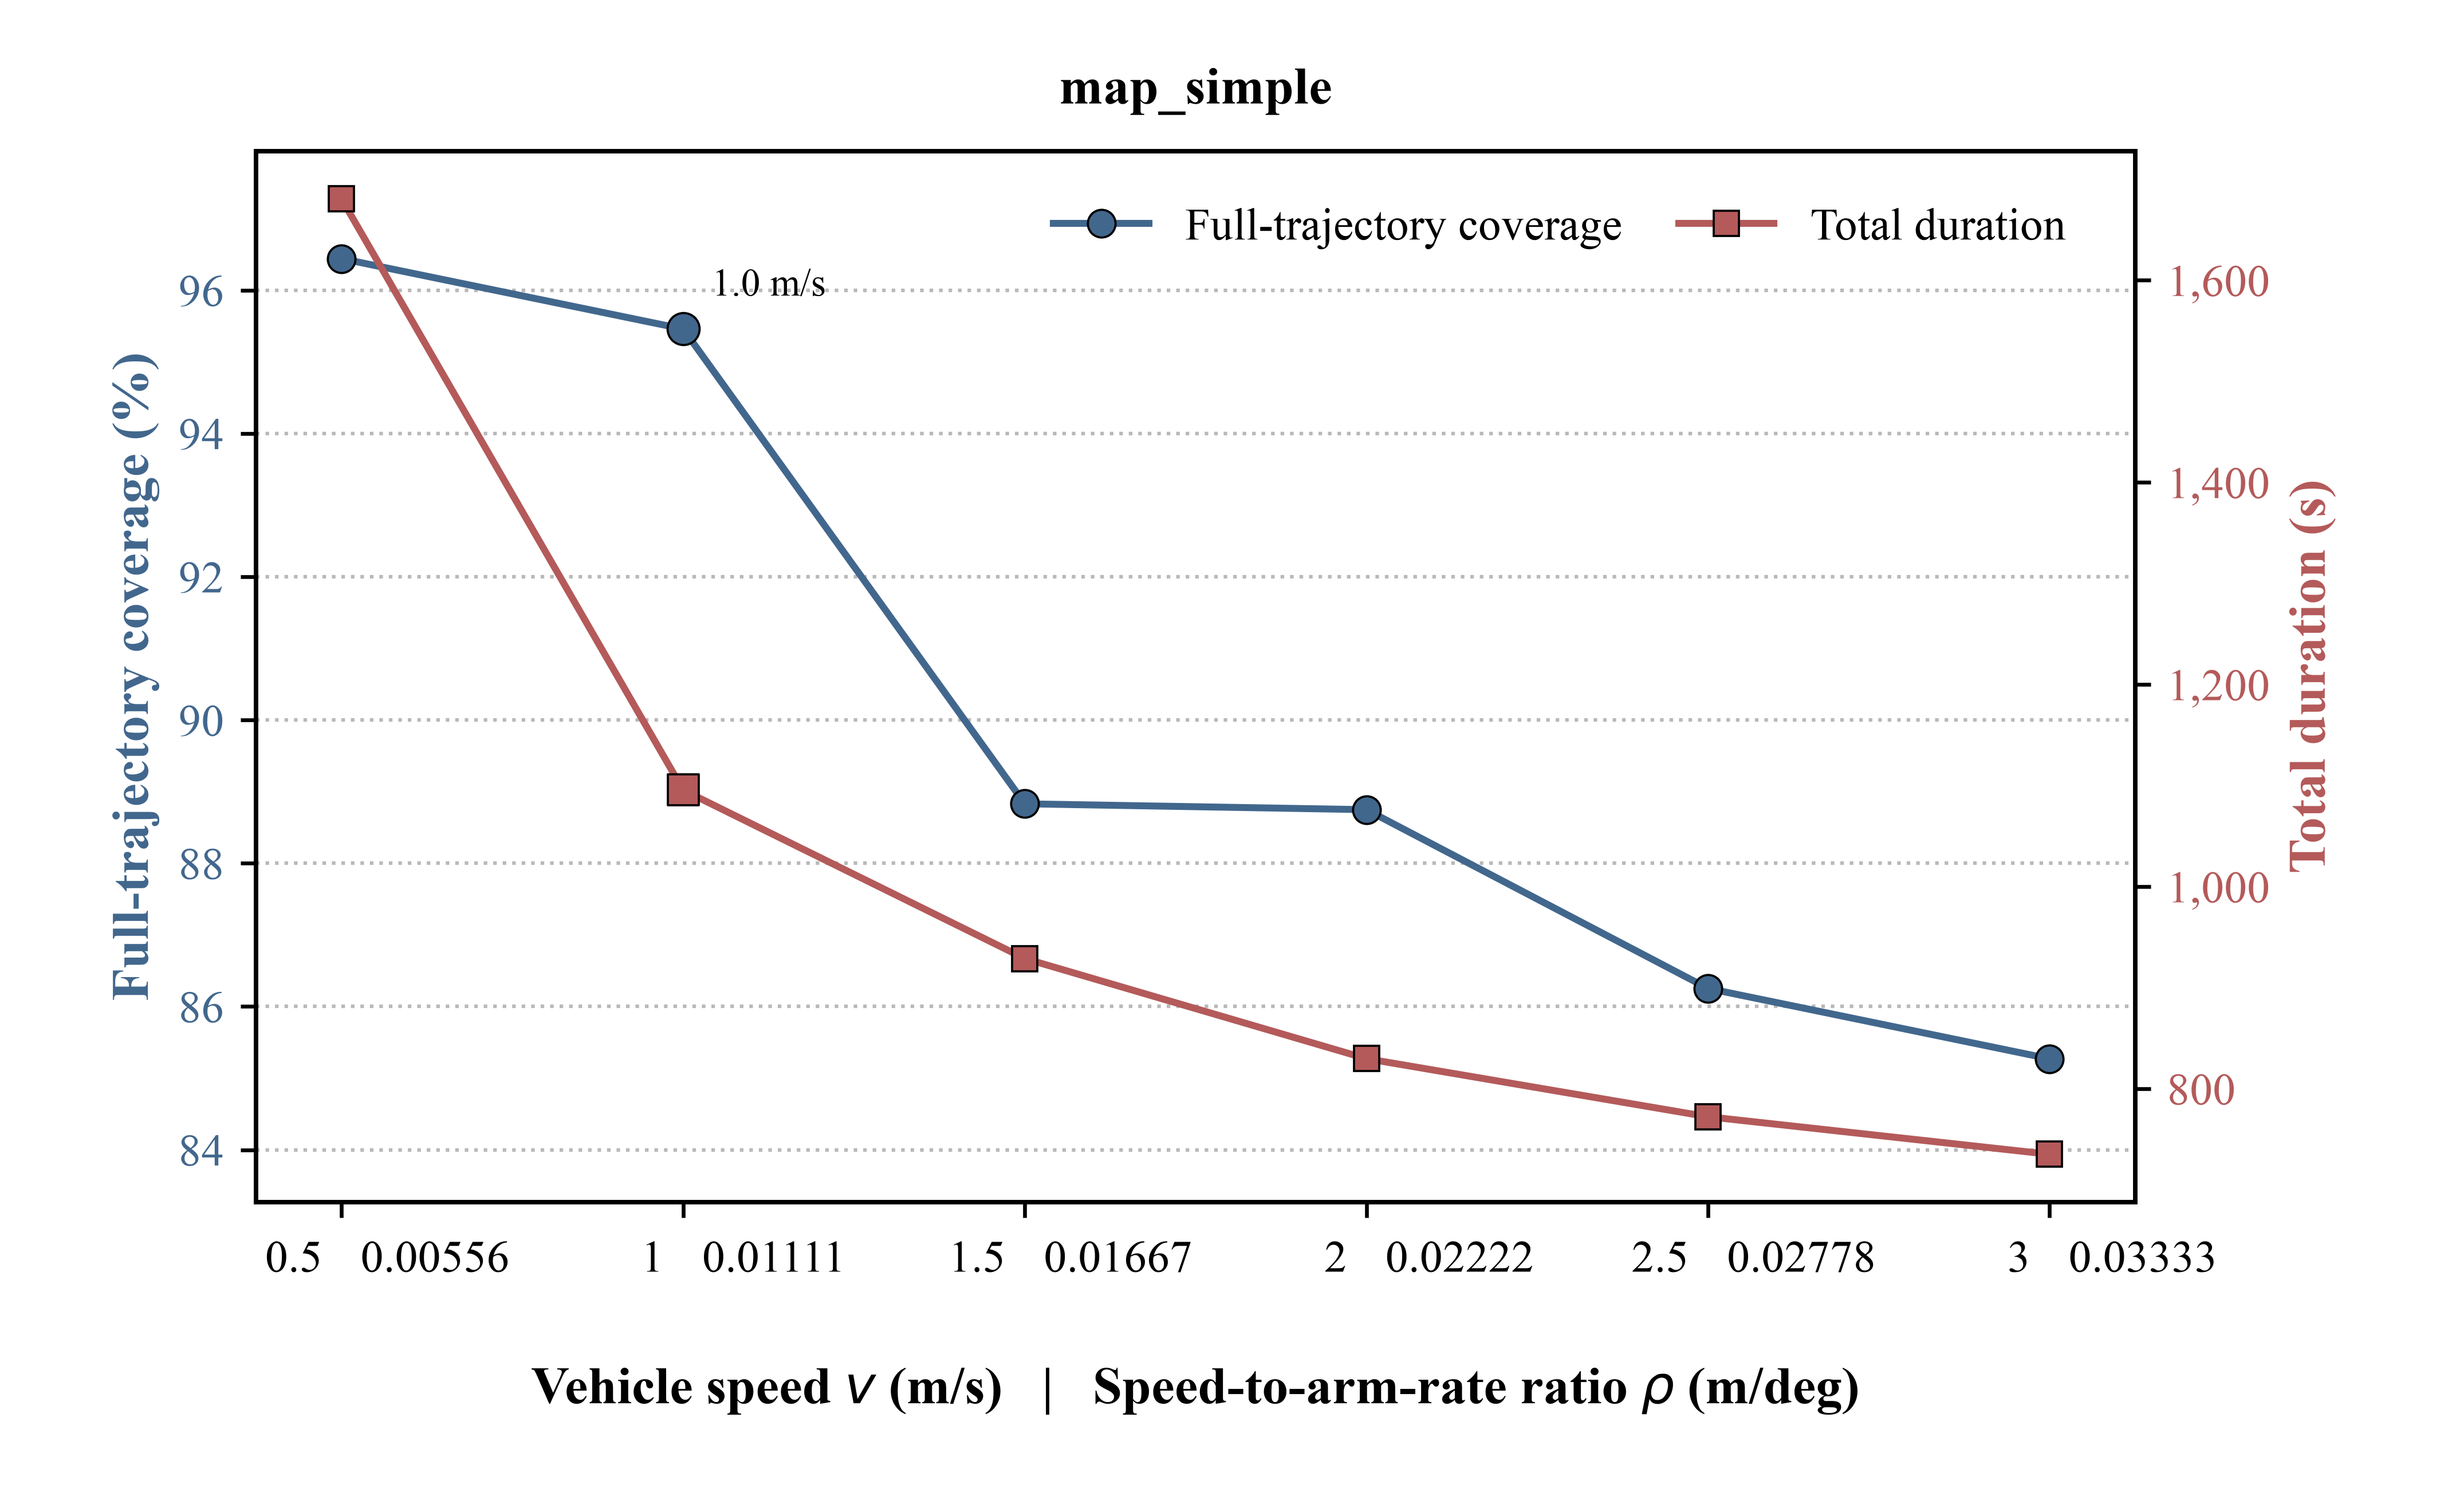
\includegraphics[width=\dimexpr\linewidth-2\fboxsep-2\fboxrule\relax]{old_figs/figure_5a_vehicle_speed_map_simple_en.png}}}\\[0.25em]
{\color{red}\scriptsize 修改前}
\end{minipage}\hfill
\begin{minipage}[t]{0.48\linewidth}\centering
{\setlength{\fboxsep}{1.2pt}\setlength{\fboxrule}{1.1pt}%
\fcolorbox{blue}{white}{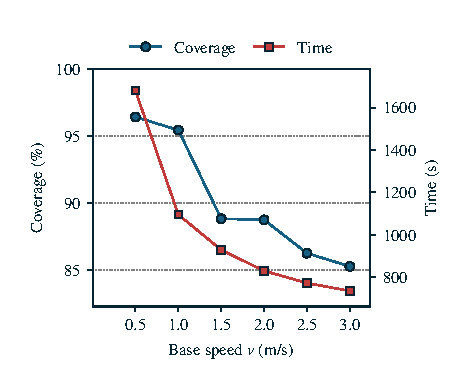
\includegraphics[width=\dimexpr\linewidth-2\fboxsep-2\fboxrule\relax]{figures/figure_5a_vehicle_speed_map_simple_en.pdf}}}\\[0.25em]
{\color{blue}\scriptsize 修改后}
\end{minipage}\par
% ===FIGPAIR END figure_5a_vehicle_speed_map_simple_en.png===
\small (a) \texttt{\DIFdelbeginFL \DIFdelFL{map\_test1}\DIFdelendFL \DIFaddbeginFL \DIFaddFL{simple}\DIFaddendFL }
\vspace{0.7em}
% ===FIGPAIR figure_5b_vehicle_speed_parkingGraph_en.png===
\par\noindent\begin{minipage}[t]{0.48\linewidth}\centering
{\setlength{\fboxsep}{1.2pt}\setlength{\fboxrule}{1.1pt}%
\fcolorbox{red}{white}{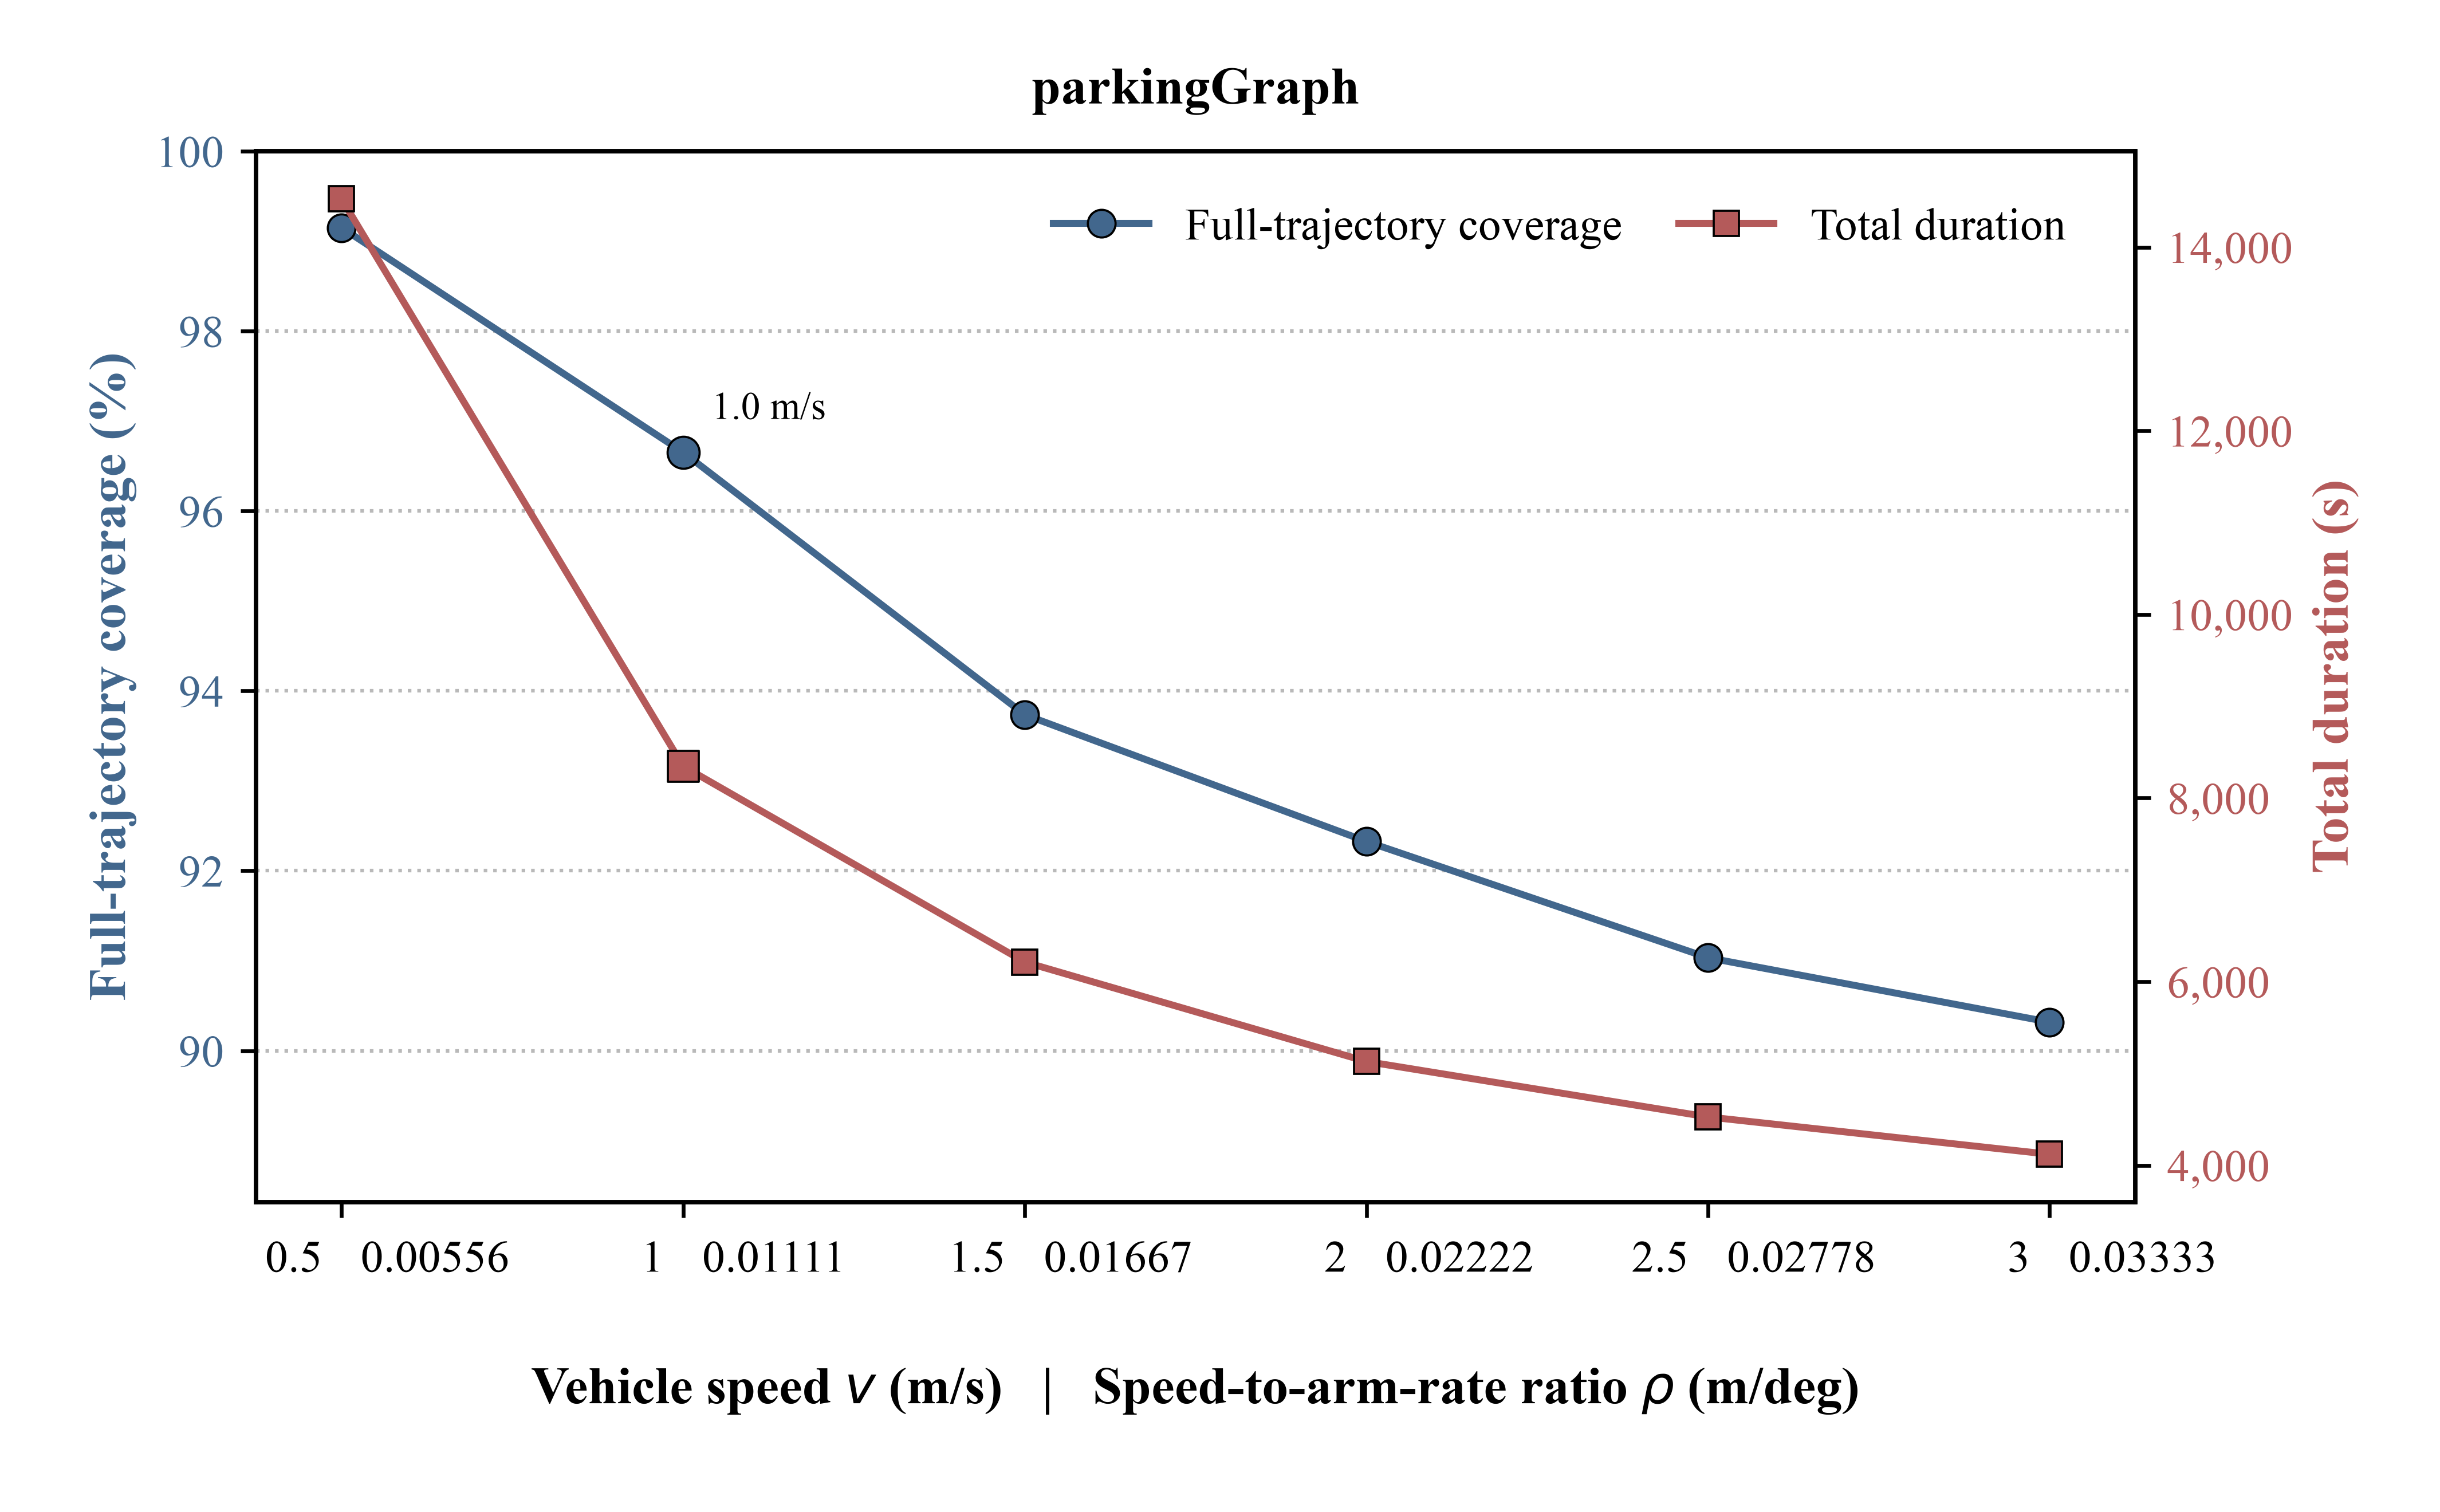
\includegraphics[width=\dimexpr\linewidth-2\fboxsep-2\fboxrule\relax]{old_figs/figure_5b_vehicle_speed_parkingGraph_en.png}}}\\[0.25em]
{\color{red}\scriptsize 修改前}
\end{minipage}\hfill
\begin{minipage}[t]{0.48\linewidth}\centering
{\setlength{\fboxsep}{1.2pt}\setlength{\fboxrule}{1.1pt}%
\fcolorbox{blue}{white}{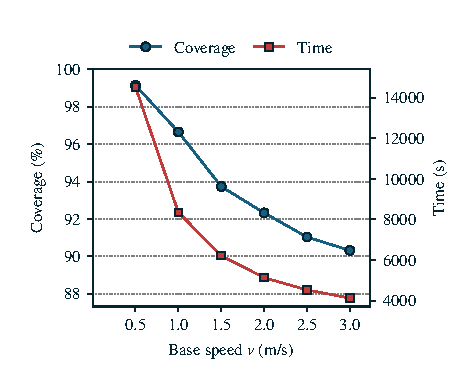
\includegraphics[width=\dimexpr\linewidth-2\fboxsep-2\fboxrule\relax]{figures/figure_5b_vehicle_speed_parkingGraph_en.pdf}}}\\[0.25em]
{\color{blue}\scriptsize 修改后}
\end{minipage}\par
% ===FIGPAIR END figure_5b_vehicle_speed_parkingGraph_en.png===
\small (b) \texttt{\DIFdelbeginFL \DIFdelFL{parkingGraph}\DIFdelendFL \DIFaddbeginFL \DIFaddFL{complex}\DIFaddendFL }

  \caption{Effect of \DIFdelbeginFL \DIFdelFL{the base-to-arm }\DIFdelendFL \DIFaddbeginFL \DIFaddFL{base--arm }\DIFaddendFL velocity \DIFdelbeginFL \DIFdelFL{ratio }\DIFdelendFL \DIFaddbeginFL \DIFaddFL{coupling }\DIFaddendFL on full-trajectory coverage and execution time\DIFaddbeginFL \DIFaddFL{, for commanded base speed $v$ with $\rho=v/\omega_a$ and fixed $r_d=0.75$~m, $L=1.20$~m, and $\omega_a=90^\circ$/s}\DIFaddendFL .\DIFdelbeginFL \DIFdelFL{The horizontal axis is \mbox{$\rho=v/\omega_a$}; the secondary top axis gives the corresponding base speed. Blue denotes full-trajectory coverage and red total execution time. Both curves use the data in Table~\mbox{\ref{tab:speed-study}}.}\DIFdelendFL }
  \label{fig:speed-study}
\end{figure}\marginpar{\scriptsize [81] 用现有速度表重画曲线并使横轴从零起，未新跑实验，也未加入没有数据的单条带曲线。}\marginpar{\scriptsize 速度曲线横轴补上 0 刻度，0 只是原点而不是观测。横轴是基座速度 v，并写出 rho 等于 v 除以 omega\_a。图注写明固定参数 r\_d=0.75 m、L=1.20 m、omega\_a=90 度/秒。}

\subsection{Discussion}

\DIFdelbegin \DIFdel{The three experiments support one central conclusion: the contribution is not simply another decomposition, but the use of coordinated base motion and end-disc swinging throughout map decomposition, trajectory generation, and swept-area evaluation, so that coverage is determined by the disc's actual continuous motion. The Fields2Cover comparison shows that }\marginpar{\scriptsize [80] 将讨论收成对应三个实验的正面三句。}\DIFdelend \DIFaddbegin \DIFadd{Relative to }\DIFaddend fixed-width strips\DIFdelbegin \DIFdel{are efficient in simple scenes, but coverage capability and connection feasibility can be constrained in dense obstacle fields; the time-varying end-disc sweep enlarges the effective workspace. The scan experiment shows that decomposition must reflect map structure and that bidirectional }\DIFdelend \DIFaddbegin \DIFadd{, the swing arm gives executable coverage on obstacle maps. Bidirectional }\DIFaddend candidates reduce the \DIFdelbegin \DIFdel{representation bias of }\DIFdelend \DIFaddbegin \DIFadd{regions left by }\DIFaddend a single scan direction. \DIFdelbegin \DIFdel{The speed experiment shows that swing-arm CPP must jointly consider route geometry and execution speed, because matching base speed }\DIFdelend \DIFaddbegin \DIFadd{Base speed relative }\DIFaddend to arm angular velocity \DIFdelbegin \DIFdel{directly determines coverage quality}\DIFdelend \DIFaddbegin \DIFadd{determines coverage and execution time}\DIFaddend .

These findings do not imply unconditional superiority over a fixed-width platform. In regular open areas, a strip-based method can obtain acceptable coverage with a shorter path and lower time. The value of the swing arm is greatest at boundaries a fixed base cannot closely follow, in obstacle-dense regions, and on wet concrete where fewer base maneuvers are desirable. Platform and parameter selection can therefore depend on site structure: large open regions favor efficient fixed-width sweeps, while complex corners and multi-obstacle regions favor arm-assisted coverage. The two could also operate in separate zones of the same floor.

The method has several limitations. First, rectangle candidates and visitation sequences are generated heuristically. They provide feasible and interpretable routes but no global optimality guarantee; many narrow corridors can still increase the rectangle count and repeated transit. Second, the input is a static two-dimensional map and does not explicitly account for workers, material stacks, localization drift, or changes in concrete condition during construction. Third, the speed analysis focuses on coverage density under base linear and arm angular velocities; it does not yet model full chassis dynamics, disc pressure, surface-quality feedback, or control error. Overall, the experiments identify explicit modeling of the end-tool sweep, area decomposition, and \DIFaddbegin \DIFadd{base--arm }\DIFaddend velocity coupling as the features that distinguish swing-arm troweling CPP from conventional fixed-width planning and define the next steps toward field deployment.

\section{Conclusion and Future Work}
\label{sec:conclusion}

Obstacles and narrow connections in complex construction maps prevent a swing-arm troweling robot from obtaining a continuous, executable coverage route from either a fixed tool footprint or a static reachability region alone. This paper presented a hierarchical CPP method for known two-dimensional environments with obstacles. Bidirectional rectangular candidates, hole filling, and connectivity completion represent the workable area; a feasible graph organizes global visitation; and first visits and repeated transit visits are instantiated as coordinated base--arm work motions and transfer motions. Planning and evaluation preserve the geometry of the base, arm, and circular disc, and coverage and nominal execution time are calculated from the disc's actual sweep along the continuous trajectory. The method thus connects map decomposition, region visitation, and end-tool coverage verification in one complete pipeline.

On \texttt{\DIFdelbegin \DIFdel{map\_test1}\DIFdelend \DIFaddbegin \DIFadd{simple}\DIFaddend } and \texttt{\DIFdelbegin \DIFdel{parkingGraph}\DIFdelend \DIFaddbegin \DIFadd{complex}\DIFaddend }, the proposed method achieves full-trajectory coverage ratios of 94.11\% and 95.73\%, respectively, and both routes pass the path check. Although the fixed-width Fields2Cover baseline generates shorter paths, its connecting segments leave the valid region by 4.51~m$^2$ and 20.00~m$^2$ on the two maps, so the associated nominal times cannot be treated as executable-route results. The comparison demonstrates the practical value of adjustable relative motion between base travel and disc operation in dense obstacle fields. In the five-map scan-strategy study, row-then-column candidates give the highest mean full-trajectory coverage (94.32\%) and the lowest mean execution time (2316.60~s), indicating that complementary row and column directions reduce representation bias; a single-direction strategy can nevertheless be preferable in some regular scenes. The speed study further shows that increasing base speed relative to arm angular velocity enlarges the spacing between sweeps and creates a coverage--time trade-off. Route geometry and execution parameters must therefore be selected together.

The current method relies on heuristic decomposition and visitation ordering and does not guarantee global optimality. It assumes a known static two-dimensional map, and its evaluation does not yet include complete chassis dynamics, localization error, disc pressure, or surface-quality feedback. Future work will jointly optimize decomposition and visitation, introduce online perception and local replanning, and validate trajectory execution and finishing quality on a physical swing-arm troweling robot. The framework may also serve as a decision-support tool for construction-map partitioning and base--arm motion configuration.


\nocite{*}
\bibliographystyle{unsrturl}
\begingroup
\small
\bibliography{refs}
\endgroup

\end{document}
